\documentclass{unmeethesis}
%\setcounter{tocdepth}{4}
%\setcounter{secnumdepth}{4}
\usepackage[titletoc]{appendix}
\makeatletter
\renewcommand\backmatter{
    \def\chaptermark##1{\markboth{%
        \ifnum  \c@secnumdepth > \m@ne  \@chapapp\ \thechapter:  \fi  ##1}{%
        \ifnum  \c@secnumdepth > \m@ne  \@chapapp\ \thechapter:  \fi  ##1}}%
    \def\sectionmark##1{\relax}}
\makeatother
%\usepackage{pdfpages}

%    Q-circuit version 2
%    Copyright (C) 2004  Steve Flammia & Bryan Eastin
%    Last modified on: 9/16/2011
%
%    This program is free software; you can redistribute it and/or modify
%    it under the terms of the GNU General Public License as published by
%    the Free Software Foundation; either version 2 of the License, or
%    (at your option) any later version.
%
%    This program is distributed in the hope that it will be useful,
%    but WITHOUT ANY WARRANTY; without even the implied warranty of
%    MERCHANTABILITY or FITNESS FOR A PARTICULAR PURPOSE.  See the
%    GNU General Public License for more details.
%
%    You should have received a copy of the GNU General Public License
%    along with this program; if not, write to the Free Software
%    Foundation, Inc., 59 Temple Place, Suite 330, Boston, MA  02111-1307  USA

% Thanks to the Xy-pic guys, Kristoffer H Rose, Ross Moore, and Daniel Müllner,
% for their help in making Qcircuit work with Xy-pic version 3.8.  
% Thanks also to Dave Clader, Andrew Childs, Rafael Possignolo, Tyson Williams,
% Sergio Boixo, Cris Moore, Jonas Anderson, and Stephan Mertens for helping us test 
% and/or develop the new version.

\usepackage{xy}
\xyoption{matrix}
\xyoption{frame}
\xyoption{arrow}
\xyoption{arc}

\usepackage{ifpdf}
\ifpdf
\else
\PackageWarningNoLine{Qcircuit}{Qcircuit is loading in Postscript mode.  The Xy-pic options ps and dvips will be loaded.  If you wish to use other Postscript drivers for Xy-pic, you must modify the code in Qcircuit.tex}
%    The following options load the drivers most commonly required to
%    get proper Postscript output from Xy-pic.  Should these fail to work,
%    try replacing the following two lines with some of the other options
%    given in the Xy-pic reference manual.
\xyoption{ps}
\xyoption{dvips}
\fi

% The following resets Xy-pic matrix alignment to the pre-3.8 default, as
% required by Qcircuit.
\entrymodifiers={!C\entrybox}

\newcommand{\bra}[1]{{\left\langle{#1}\right\vert}}
\newcommand{\ket}[1]{{\left\vert{#1}\right\rangle}}
    % Defines Dirac notation. %7/5/07 added extra braces so that the commands will work in subscripts.
\newcommand{\qw}[1][-1]{\ar @{-} [0,#1]}
    % Defines a wire that connects horizontally.  By default it connects to the object on the left of the current object.
    % WARNING: Wire commands must appear after the gate in any given entry.
\newcommand{\qwx}[1][-1]{\ar @{-} [#1,0]}
    % Defines a wire that connects vertically.  By default it connects to the object above the current object.
    % WARNING: Wire commands must appear after the gate in any given entry.
\newcommand{\cw}[1][-1]{\ar @{=} [0,#1]}
    % Defines a classical wire that connects horizontally.  By default it connects to the object on the left of the current object.
    % WARNING: Wire commands must appear after the gate in any given entry.
\newcommand{\cwx}[1][-1]{\ar @{=} [#1,0]}
    % Defines a classical wire that connects vertically.  By default it connects to the object above the current object.
    % WARNING: Wire commands must appear after the gate in any given entry.
\newcommand{\gate}[1]{*+<.6em>{#1} \POS ="i","i"+UR;"i"+UL **\dir{-};"i"+DL **\dir{-};"i"+DR **\dir{-};"i"+UR **\dir{-},"i" \qw}
    % Boxes the argument, making a gate.
\newcommand{\meter}{*=<1.8em,1.4em>{\xy ="j","j"-<.778em,.322em>;{"j"+<.778em,-.322em> \ellipse ur,_{}},"j"-<0em,.4em>;p+<.5em,.9em> **\dir{-},"j"+<2.2em,2.2em>*{},"j"-<2.2em,2.2em>*{} \endxy} \POS ="i","i"+UR;"i"+UL **\dir{-};"i"+DL **\dir{-};"i"+DR **\dir{-};"i"+UR **\dir{-},"i" \qw}
    % Inserts a measurement meter.
    % In case you're wondering, the constants .778em and .322em specify
    % one quarter of a circle with radius 1.1em.
    % The points added at + and - <2.2em,2.2em> are there to strech the
    % canvas, ensuring that the size is unaffected by erratic spacing issues
    % with the arc.
\newcommand{\measure}[1]{*+[F-:<.9em>]{#1} \qw}
    % Inserts a measurement bubble with user defined text.
\newcommand{\measuretab}[1]{*{\xy*+<.6em>{#1}="e";"e"+UL;"e"+UR **\dir{-};"e"+DR **\dir{-};"e"+DL **\dir{-};"e"+LC-<.5em,0em> **\dir{-};"e"+UL **\dir{-} \endxy} \qw}
    % Inserts a measurement tab with user defined text.
\newcommand{\measureD}[1]{*{\xy*+=<0em,.1em>{#1}="e";"e"+UR+<0em,.25em>;"e"+UL+<-.5em,.25em> **\dir{-};"e"+DL+<-.5em,-.25em> **\dir{-};"e"+DR+<0em,-.25em> **\dir{-};{"e"+UR+<0em,.25em>\ellipse^{}};"e"+C:,+(0,1)*{} \endxy} \qw}
    % Inserts a D-shaped measurement gate with user defined text.
\newcommand{\multimeasure}[2]{*+<1em,.9em>{\hphantom{#2}} \qw \POS[0,0].[#1,0];p !C *{#2},p \drop\frm<.9em>{-}}
    % Draws a multiple qubit measurement bubble starting at the current position and spanning #1 additional gates below.
    % #2 gives the label for the gate.
    % You must use an argument of the same width as #2 in \ghost for the wires to connect properly on the lower lines.
\newcommand{\multimeasureD}[2]{*+<1em,.9em>{\hphantom{#2}} \POS [0,0]="i",[0,0].[#1,0]="e",!C *{#2},"e"+UR-<.8em,0em>;"e"+UL **\dir{-};"e"+DL **\dir{-};"e"+DR+<-.8em,0em> **\dir{-};{"e"+DR+<0em,.8em>\ellipse^{}};"e"+UR+<0em,-.8em> **\dir{-};{"e"+UR-<.8em,0em>\ellipse^{}},"i" \qw}
    % Draws a multiple qubit D-shaped measurement gate starting at the current position and spanning #1 additional gates below.
    % #2 gives the label for the gate.
    % You must use an argument of the same width as #2 in \ghost for the wires to connect properly on the lower lines.
\newcommand{\control}{*!<0em,.025em>-=-<.2em>{\bullet}}
    % Inserts an unconnected control.
\newcommand{\controlo}{*+<.01em>{\xy -<.095em>*\xycircle<.19em>{} \endxy}}
    % Inserts a unconnected control-on-0.
\newcommand{\ctrl}[1]{\control \qwx[#1] \qw}
    % Inserts a control and connects it to the object #1 wires below.
\newcommand{\ctrlo}[1]{\controlo \qwx[#1] \qw}
    % Inserts a control-on-0 and connects it to the object #1 wires below.
\newcommand{\targ}{*+<.02em,.02em>{\xy ="i","i"-<.39em,0em>;"i"+<.39em,0em> **\dir{-}, "i"-<0em,.39em>;"i"+<0em,.39em> **\dir{-},"i"*\xycircle<.4em>{} \endxy} \qw}
    % Inserts a CNOT target.
\newcommand{\qswap}{*=<0em>{\times} \qw}
    % Inserts half a swap gate.
    % Must be connected to the other swap with \qwx.
\newcommand{\multigate}[2]{*+<1em,.9em>{\hphantom{#2}} \POS [0,0]="i",[0,0].[#1,0]="e",!C *{#2},"e"+UR;"e"+UL **\dir{-};"e"+DL **\dir{-};"e"+DR **\dir{-};"e"+UR **\dir{-},"i" \qw}
    % Draws a multiple qubit gate starting at the current position and spanning #1 additional gates below.
    % #2 gives the label for the gate.
    % You must use an argument of the same width as #2 in \ghost for the wires to connect properly on the lower lines.
\newcommand{\ghost}[1]{*+<1em,.9em>{\hphantom{#1}} \qw}
    % Leaves space for \multigate on wires other than the one on which \multigate appears.  Without this command wires will cross your gate.
    % #1 should match the second argument in the corresponding \multigate.
\newcommand{\push}[1]{*{#1}}
    % Inserts #1, overriding the default that causes entries to have zero size.  This command takes the place of a gate.
    % Like a gate, it must precede any wire commands.
    % \push is useful for forcing columns apart.
    % NOTE: It might be useful to know that a gate is about 1.3 times the height of its contents.  I.e. \gate{M} is 1.3em tall.
    % WARNING: \push must appear before any wire commands and may not appear in an entry with a gate or label.
\newcommand{\gategroup}[6]{\POS"#1,#2"."#3,#2"."#1,#4"."#3,#4"!C*+<#5>\frm{#6}}
    % Constructs a box or bracket enclosing the square block spanning rows #1-#3 and columns=#2-#4.
    % The block is given a margin #5/2, so #5 should be a valid length.
    % #6 can take the following arguments -- or . or _\} or ^\} or \{ or \} or _) or ^) or ( or ) where the first two options yield dashed and
    % dotted boxes respectively, and the last eight options yield bottom, top, left, and right braces of the curly or normal variety.  See the Xy-pic reference manual for more options.
    % \gategroup can appear at the end of any gate entry, but it's good form to pick either the last entry or one of the corner gates.
    % BUG: \gategroup uses the four corner gates to determine the size of the bounding box.  Other gates may stick out of that box.  See \prop.

\newcommand{\rstick}[1]{*!L!<-.5em,0em>=<0em>{#1}}
    % Centers the left side of #1 in the cell.  Intended for lining up wire labels.  Note that non-gates have default size zero.
\newcommand{\lstick}[1]{*!R!<.5em,0em>=<0em>{#1}}
    % Centers the right side of #1 in the cell.  Intended for lining up wire labels.  Note that non-gates have default size zero.
\newcommand{\ustick}[1]{*!D!<0em,-.5em>=<0em>{#1}}
    % Centers the bottom of #1 in the cell.  Intended for lining up wire labels.  Note that non-gates have default size zero.
\newcommand{\dstick}[1]{*!U!<0em,.5em>=<0em>{#1}}
    % Centers the top of #1 in the cell.  Intended for lining up wire labels.  Note that non-gates have default size zero.
\newcommand{\Qcircuit}{\xymatrix @*=<0em>}
    % Defines \Qcircuit as an \xymatrix with entries of default size 0em.
\newcommand{\link}[2]{\ar @{-} [#1,#2]}
    % Draws a wire or connecting line to the element #1 rows down and #2 columns forward.
\newcommand{\pureghost}[1]{*+<1em,.9em>{\hphantom{#1}}}
    % Same as \ghost except it omits the wire leading to the left. 

\usepackage{amsmath}
\usepackage{amsfonts,amssymb,amsthm, bbm,braket}
\usepackage{graphicx}   % need for figures
\usepackage{subfigure}  % and subfigures
\usepackage{amsbsy} % for bold greek letters
\usepackage[bold]{hhtensor}
\usepackage[multiple]{footmisc}
\usepackage{epigraph} % inspirational quotes
%\usepackage[all]{xy} % commutative diagrams and dynkin diagrams
\usepackage{tikz} % commutative and dynkin diagrams
\usepackage{mathtools} % math equal, inclusion arrows
\usepackage{dsfont}
\usepackage{etoolbox}
\usepackage{adjustbox} % for \bwedge
\usepackage{float}
\usepackage{faktor}
\usepackage{xcolor}
\usepackage{lipsum} % for block quotes

%--MACROS--

\preto\chapter{\undef\rep} % \rep must be redefined at the beginning of every chapter if needed

\newcommand\id{\mathbbm 1}
\newcommand\Tr{\mathrm{Tr}}
\newcommand{\ketbra}[2]{\ket{#1}\bra{#2}}
\newcommand\krep{\sigma} % representation of subgroup
\newcommand{\gr}[2]{\text{#1}(#2)} % linear group
\newcommand{\homsp}[4]{\text{#1}(#2)/\text{#3}(#4)} % homogeneous space
\newcommand{\al}\mathfrak % Lie algebra
\newcommand{\ind}[3]{\text{Ind}_{#2}^{#3} {#1}} % induced representation
\newcommand{\res}[3]{\text{Res}^{#2}_{#3} {#1}} % restricted representation
\newcommand{\coind}[3]{\text{Coind}_{#2}^{#3} {#1}} % coinduced representation
\newcommand\mat[2]{\mathbb{M}_{#1 \times #2}(\mathbb{R})} % real matrices; \matr is already defined
\newcommand\matc[2]{\mathbb{M}_{#1 \times #2}(\mathbb{C})} % complex matrices
\newcommand\adrep{\text{ad}\,} % adjoint representation
\newcommand\Adrep{\text{Ad}\,} % Adjoint representation
\newcommand{\kil}[2]{\text{Kill}(#1,#2)} % Killing form
\newcommand{\ran}{\text{rank}\,} % rank
\newcommand\norm[1]{\|#1\|}
\newcommand\hilb{\mathcal{H}}
\newcommand\herm{\mathbb H(\hilb)}
\newcommand\rker[1]{\mathcal{K}_{#1}} % reproducing kernel
\newcommand\dgg{^{\dagger}} % Hermitian conjugate
\newcommand{\bwedge}{\mathord{\adjustbox{valign=m,totalheight=.5\baselineskip}{$\bigwedge$}}} % medium-sized wedge

% Round bra-ket
\newcommand{\rket}[1]{|#1)}
\newcommand{\rbra}[1]{(#1|}
\newcommand{\rketbra}[2]{\rket{#1}\rbra{#2}}

%---------------------------Chris' Macro from the quantum Bochner paper

\newcommand\unit{\mathbb U(\mathcal H)}
\newcommand\den{\mathbb D(\mathcal H)}
\newcommand\eff{\mathbb E(\mathcal H)}
\newcommand\proj{\mathbb P(\mathcal H)}
\newcommand\povm{\mathrm{POVM}(\mathcal H)}
\newcommand\pvm{\mathrm{PVM}(\mathcal H)}
\newcommand\range{\mathrm{Ran}}
\newcommand\domain{\mathrm{Dom}}
\newcommand\conv{\mathrm{conv}}
\newcommand\spec{\mathrm{spec}}
\newcommand\freq{\frac{2\pi i}{n}}
\newcommand\w[1]{e^{\freq #1}}
\newcommand\ip[2]{\langle#1 | #2\rangle}
\newcommand\op[2]{|#1\rangle\!\langle#2|}
\newcommand\abs[1]{\left|#1\right|}
\newcommand\av[1]{\left\langle #1 \right\rangle}
\newcommand\conj[1]{#1^*}
%---------------------------

\newcommand\nd{\color{red}}
\newcommand\cmc{\color{magenta}}
\newcommand\csj{\color{blue}}

%--U(4) root color

\definecolor{onetwo}{RGB}{33,140,141}
\definecolor{twothree}{RGB}{239,113,38}
\definecolor{threefour}{RGB}{71,62,63}
\newcommand\onetwo{\color{onetwo}}
\newcommand\twothree{\color{twothree}}
\newcommand\threefour{\color{threefour}}
\def\cmccomment#1{{\tt#1}}

%--ENVIRONMENTS--

\newtheorem{definition}{Definition}
\newtheorem{corollary}{Corollary}
\newtheorem{theorem}{Theorem}
\newtheorem{lemma}{Lemma}
\newtheorem{proposition}{Proposition}
\newtheorem{question}{Question}

\usepackage[breaklinks=true]{hyperref}
\hypersetup{
  colorlinks   = true, %Colours links instead of ugly boxes
  urlcolor     = blue, %Colour for external hyperlinks
  linkcolor    = blue, %Colour of internal links
  citecolor   = magenta %Colour of citations
}
\renewcommand{\sectionautorefname}{\S}
\renewcommand{\subsectionautorefname}{\S}
\renewcommand{\subsubsectionautorefname}{\S}

\begin{document}

%\includepdf[pages={1}]{approval.pdf}

\frontmatter

\title{Quantum Phase Space Representations and Their Negativities}

\author{Ninnat Dangniam}

\degreesubject{Ph.D., Physics}

\degree{Doctor of Philosophy \\ Physics}

\documenttype{Dissertation}

\previousdegrees{B.S., Physics, University of Oregon, 2011 \\
B.S., Mathematics, University of Oregon, 2011}

\date{May 2018}

\maketitle

\makecopyright

%{\cmc Once CJ has read this again and you have sent the thing off to the committee (by Feb 15, let's say), you will need to check through the whole thing carefully to bring everything into consistency: mathematical notation consistent throughout, punctuation (especially of equations) and grammar styles the same throughout.  For example, you need to decide whether you are referring to sections with Section or with the symbol.  You need to adhere to the convention that the m-dash (---) is used for interruptions in a sentence; there are m-dashes at both ends of the interruptions, and these are not separated by spaces from surrounding text.  Among other things, I think you need all your footnotes to start with a capital letter and end with a period, even if they are phrases; you're currently using many footnotes to accommodate what might better be parenthetical phrases, and you might think about actually making some of them parenthetical phrases (since they will be noticed better that way).

%You probably also should look through the references for things like the following.  Shouldn't Braunstein and Bravyi have different abbreviations?  What about the title of Bra06, which has some uncompiled LaTeX in it?

%You are going to need of you are going to capitalize boson, bosonic, fermion, and fermionic and be consistent throughout.}

%{\nd I have fixed all the missing diacritics and strayed uncompiled LaTeX that I could find in the bibliography. I wasn't yet able to distinguish the abbreviations of Braunstein and Bravyi; using \textbackslash disambiguate throws me a compiling error.

%I went through all the footnotes and put them into the main text whenever appropriate. But I have a feeling that my decisions might not be that consistent throughout, so I will go though everything again. I've so far reread and fixed the first 2 chapters. FYI, CJ didn't have a chance to finish rereading the thesis before I sent it off to the committee.}

\begin{acknowledgments}
Before anything else, I would like to thank my parents, who not only believe in me, but also support whatever life choice I pursue, both emotionally and financially, something that not all parents can do.

I would like to express my deepest gratitude to the three C's: my advisor Carlton Caves, Christopher Ferrie, and Christopher Jackson,
%\footnote{All their first names begin with C! (not 100 factorial).}
without whom this dissertation would not have been possible.  It has been a valuable experience to be exposed to contrasting styles of mentoring, with Carl's high standards and emphasis on understanding explicit examples instead of getting caught up in generalities---a ``pedestrian approach" as he humbly puts it---on one hand, and Chris Ferrie's more whimsical, intuitive style on the other hand.  Although it has only been a year since I started collaborating with Chris Jackson, I always enjoy his presence and contagious passion on all things mathematical.  He also thoroughly read and gave a detailed feedback on every technical chapter of the dissertation. I would also like to thank the members of my dissertation committee: Carl, Chris Ferrie, Akimasa Miyake, Cristopher Moore, and Daniel Finley for taking time out of their busy schedules to read this dissertation.

My time at UNM has been one of the best times in my life, and everyone here is to be thanked for that. I have learned much from the faculty and post-docs in CQuIC (in addition to the three C's), especially Ivan Deutsch, Andrew Landahl, Akimasa Miyake, Cristopher Moore, Howard Barnum, Robin Blume-Kohout, Joshua Combes, and Rafael Alexander. It is also my pleasure to interact with other UNM faculty members, in particular, David Dunlap and Rouzbeh Allahverdi. My special thanks also go to fellow graduate students Jonathan Gross for just being an all-around brilliant groupmate, Jacob Miller for all the interesting random conversations, and Adrian Chapman and Qi Xiaodong for being officemates and surviving together. I thank Jonathan, Qi, Travis Scholten, and Anupam Mitra for organizing the outstanding computing workshop, and last but not least, the CQuIC Program Specialist, Gloria Cordova, for putting up with us and making our lives here easier.

I am indebted to Stephen Bartlett, Andrew Doherty, Steve Flammia, and everyone at the Quantum Science Research Group at the University of Sydney for the hospitality during my two visits.
\end{acknowledgments} 

\newpage
\begin{abstract}

\noindent A classical simulation scheme of quantum computation given a restricted set of states and measurements may be---occasionally, but only occasionally---interpreted naturally as a statistical simulation of positive quasi-probability distributions on a phase space. In this dissertation, we explore phase space representations for finite-dimensional quantum systems and their negativities beyond the usual analogues of the Wigner function.

The first line of study focuses on a characterization tool for valid quasi-probability distributions of (possibly mixed) quantum states. A quantum generalization of Bochner's theorem from classical probability theory simultaneously characterizes both the set of valid Wigner functions and the subset of positive ones. We extend this theorem to discrete phase spaces based on projective representations of abelian groups, including the discrete Wigner functions of Gross (J. Math. Phys. 47, 122107 (2006)) and Gibbons \emph{et al.} (Phys. Rev. A 70, 062101 (2004)).

The rest of the dissertation is then dedicated to phase space representations covariant with respect to a general Lie group. This means, in particular, that operators that lie in the same orbit of the group have the same amount of negativity in their quasi-probabilities---a natural requirement if one would like to interpret negativity as non-classicality, and the group action as a classical dynamics. We show that the construction due to Brif and Mann (Phys. Rev. A 59, 971 (1999)) of group covariant phase space representations satisfying the so-called Stratonovich-Weyl correspondence is essentially unique, given the group and an input state in the relevant representation. As an application, we construct quasi-probability representations on a compact phase space of fermionic Gaussian states tailored to a classically simulatable problem of fermionic linear optics and find that, in the first non-trivial case of four fermionic modes, the quasi-probabilities of the Gaussian states exhibit a considerable amount of negativity.

%\cmc{I think the style in abstracts is to put in references explicitly, in the most abbreviated form, since the abstract might appear separately from the rest of the document.}
\end{abstract}



\tableofcontents

\listoffigures

\mainmatter

%\input{chapters/symbol-list}

\chapter{Introduction}\label{ch:intro}
\setlength\epigraphwidth{9cm}
\epigraph{[The formalism of quantum mechanics] is a peculiar mixture describing in part realities of Nature, in part incomplete human information about Nature -- all scrambled up by Heisenberg and Bohr into an omelette that nobody has seen how to unscramble.}{--- Edwin T. Jaynes}
% "Probability in Quantum Theory" in Complexity, Entropy, and the Physics of Information, W. H. Zurek (ed.), Addison-Wesley, Redwood City, CA, p. 381

%------------------------------------
%\section{็Quantum theory in phase space}
%------------------------------------

Just as classical mechanics can be formulated in many different ways---Newtonian, Lagrangian, Hamiltonian, to give some examples---so, too, can quantum mechanics~\cite{styer2002nine}.  Different formulations bring to the fore different aspects of the theory even as they obscure others. The focus of this dissertation is on the phase space formulations of quantum theory, in which the usual complex Hilbert space retreats into the background, and a picture resembling that of classical statistical mechanics emerges.

The concept of a phase space has its roots in classical Hamiltonian mechanics. It gives a complete description of a system in terms of conjugate variables, $\{q_j\}$ and $\{p_j\}$, defined by the Poisson bracket
\begin{align}
\{ q_j,p_k \}_{PB} = \delta_{jk},
\end{align}
where
\begin{align}
	\{ f,g \}_{PB} &= \sum_j \frac{\partial f}{\partial q_j} \frac{\partial g}{\partial p_j} - \frac{\partial g}{\partial q_j} \frac{\partial f}{\partial p_j}.
\end{align}
The word ``phase" in ``phase space" originated from Boltzmann when he described instantaneous points in the Lissajous pattern of two harmonic oscillators by their instantaneous relative phase. The trajectory of these \emph{phase points} fills the entire space bounded by the oscillators' amplitudes when the ratio of the frequencies of the two oscillators is irrational, a circumstance which would later become Boltzmann's ergodic hypothesis \cite{nolte_tangled_2010}.

The Heisenberg uncertainty relation prevents a deterministic phase space description of a quantum system completely localized in both of its conjugate variables, such as position and momentum---there are no quantum phase points!
This does not, however, prevent a statistical formulation of quantum theory on a phase space. The first example was developed by Wigner, who showed that quantum expectation values can be calculated as averages over phase space distributions, now known as \emph{Wigner functions} \cite{wigner_quantum_1932}. Wigner functions are not true probability densities and are said to be \emph{quasi-probabilities} as they take on negative values for some states. Moyal \cite{moyal_quantum_1949} noticed that Wigner's quasi-probability map is the inverse of Weyl's quantization rule that maps distributions to quantum operators \cite{weyl_quantenmechanik_1927}. Independently, Moyal and Groenewold \cite{groenewold_principles_1946} established the Wigner-Weyl phase space picture as an autonomous formulation of quantum mechanics. (For the interested reader, historically important papers, each accompanied by a brief annotation, are collected in \cite{zachos2005quantum}.) 

The notion of a Wigner function, which to many is synonym to that of a quasi-probability representation, has been generalized to physical systems with other symmetries, for example, the Poincar{\'e} symmetry of special relativity~\cite{kim1991phase,schroeck1996quantum}. The spherical phase space representation \cite{stratonovich_distributions_1957} and discrete phase spaces---the one by Hannay and Berry \cite{hannay_quantization_1980} being the first that appeared in the literature---are one of the many generalizations \cite{ferrie_quasi-probability_2011} of the Wigner function to finite-dimensional (spin) systems.

%The phase space representation is by now an essential tool in the field of quantum optics \cite{cahill_density_1969,sudarshan_equivalence_1963,hillery_distribution_1984,lee_theory_1995}.

 %Ones of the most popular quasi-probability representations of quantum theory such as the Galuber-Sudarshan P \cite{cahill_density_1969,sudarshan_equivalence_1963} and Husimi Q \cite{husimi_formal_1940} distributions share the same phase space $\mathbb{R}^{2n}$ with the Wigner function, and there are many discretized variants of the phase space.

There is a tendency to associate negativity of quasi-probability distributions with non-classicality of quantum states. In the Glauber-Sudarshan \emph{P representation} \cite{glauber_coherent_1963, sudarshan_equivalence_1963}, the only states that make $P$ a true probability distribution are mixtures (convex combinations) of coherent states $\{\ket{\alpha}\}$. Introduced by Schr{\"o}dinger as ``the most classical" states of a harmonic oscillator, coherent states are states with minimal uncertainty, equally distributed between the two quadratures. Glauber coined the term ``coherent states" and ascribed them to quantum states of light that can be modeled by a stochastic classical electromagnetic field. Non-coherent states such as squeezed states and photon number states have negative $P$ distributions and are often thought of as non-classical states. %Squeezed states have negative P distributions and can offer better sensitivity over classical light in some metrological tasks \cite{walls2007quantum}.
The difficulty in associating negativity and non-classicality is that the choice of the quasi-probability representation is not unique. A state with a negative quasi-probability distribution in one representation may have a positive quasi-probability distribution in another representation. For instance, the Wigner functions of all Gaussian states including the squeezed ones are non-negative. In fact, in the Husimi $Q$ representation \cite{husimi_formal_1940}:
\begin{align}
	Q_{\rho}(\alpha) &= \braket{\alpha| \rho |\alpha}
\end{align}
every state has a positive distribution. So negativity of a quasi-probability distribution \emph{per se} cannot be an indicator of non-classicality. An operational approach can offer a resolution to this difficulty. What we can do with a quantum state depends on which measurements we are allowed to make, and vice versa. So an operationally motivated definition of non-classicality must consider both states and measurements in conjunction.

Once the full quantum formalism is taken into account, does there exist a quasi-probability representation that displays no negativity at all? Intuitively, this cannot be the case because otherwise quantum theory would be reduced to a classical statistical theory. Indeed, the answer for finite dimensions was given in the negative, independently in \cite{spekkens_negativity_2008} and \cite{ferrie_frame_2008,ferrie_framed_2009}, while \cite{ferrie_necessity_2010} generalizes the latter proof to infinite dimensional Hilbert spaces. Thus, the problem shifts to finding a \emph{non-negative subtheory}: a subset of quantum states and measurements that are represented by non-negative quasi-probability distributions \cite{wallman_non-negative_2012}. A phase space representation automatically supplies a classical statistical theory, a hidden variable theory (a non-contextual hidden variable theory in the sense of Spekkens \cite{spekkens_negativity_2008} to be exact, since a quasi-probability mapping of an operator is defined to be one-one) for the non-negative subtheory in that representation (if exists). Thus, a phase space representation suggests a natural boundary between what is classical and what is intrinsically quantum.

Fast-forwarding to the present, an interest in non-negative subtheories has been renewed by the possibility of a quantum computer, a machine that makes use of fragile quantum effects which typically do not survive in an uncontrolled en\-vi\-ron\-ment, to solve particular problems faster than any known classical method. For simplicity, what we mean by a quantum computer is a \emph{universal} one that can simulate any quantum computer with at most a resource that is polynomial in the size $n$ of the input, or more precisely $\mathcal{O}(n^k)$ for some positive number $k$. We write $f(n)=\mathcal{O}(g(n))$ and say that the function $f(n)$ grows as $g(n)$ if there is a positive constant $c$ such that, for some $n_0$,
\begin{align}
	|f(n)| \le c|g(n)|,
\end{align}
when $n>n_0$, that is, asymptotically. Polynomial functions are closed in the sense that a composition of polynomials is also a polynomial. So in a very coarse-grained point of view, if we deem algorithms that run in time proportional to the input size ($f(n) = n$) efficient, then it is natural to call a concatenation of these linear-time algorithms efficient as well. Admittedly, the degree of the polynomial can be very high, but phenomenologically this notion of efficiency seems to be robust, as most polynomial-time algorithms turn out to be practical \cite{AB,aaronson2013democritus}.

\begin{figure}[H]
	\begin{center}
		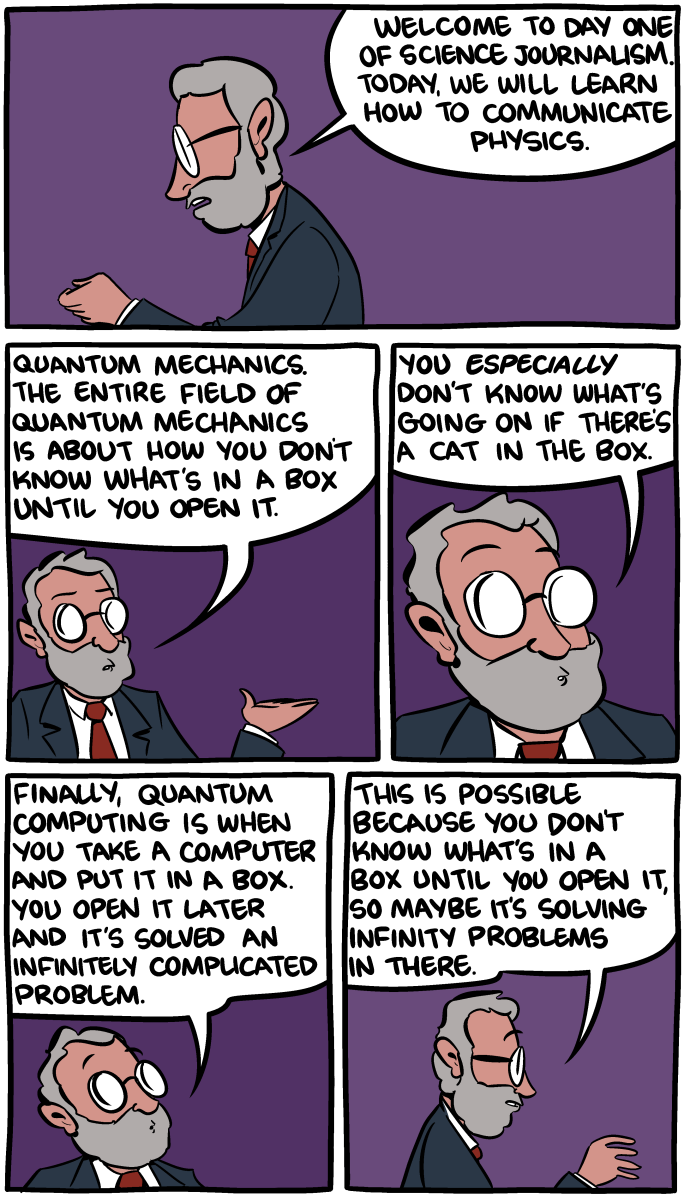
\includegraphics[width=0.5\textwidth]{img/smbc-science-communication.png}
			\caption{In a quantum world, a cat can be dead or alive; knowing that an electron here is in the ``spin up" state instantaneously collapses an electron on the other side of the universe to the ``spin down" state.
			Prompted by this description of the quantum world, an intelligent seven-year-old might say: ``What's the big deal? The cat is either alive or dead. We just couldn't tell until we look at it. Also, the pair of electrons is no different from a pair of gloves. If I know that one of the gloves is left handed, the other one must be right handed."
			And the kid would be right! Classical randomness and classical correlation suffice to explain any outcome of a quantum measurement done in a single fixed basis.
			(The comic is reprinted with permission from the author \cite{SMBC}.)}
			\label{fig:smbc-comics}
	\end{center}
\end{figure}

With a growing list of problems that are easier to solve on a quantum computer than a classical one \cite{jordan2017zoo}, it is natural to ask: where does the quantum speed-up come from?  For concreteness, let us assume that our quantum computer is composed of $n$ qubits i.e. spin-1/2 systems in pure states.  What a quantum computer of this sort does is nothing but rotating a $2^n$-dimensional complex vector around.  Thus we might look for a physical system with a similar mathematical structure and see why we cannot use it to achieve the same effect as quantum speed-up. For example, classical waves are also described by complex amplitudes. So why can't we let classical waves perform quantum computation? The problem is that the number of modes needed to simulate the Hilbert space of $n$ qubits scales exponentially in $n$ because classical waves lack the entanglement that makes up the exponentially large composite Hilbert space \cite{jozsa1997entanglement,blume-kohout_climbing_2002}.

%Classical waves can superpose but the number of modes needed to simulate the Hilbert space scales exponentially because they lack the tensor product structure ---that is, entanglement-- that makes up an exponentially large composite Hilbert space \cite{jozsa1997entanglement,blume-kohout_climbing_2002}. Soon after it was shown that entanglement, quantified by a suitable entanglement measure, is necessary to achieve an exponential speed-up in pure state quantum computation \cite{jozsa_role_2003,vidal_efficient_2003}. \cite{van_den_nest_universal_2013} showed that quantum computation with little entanglement according to continuous entanglement measures can still perform a universal quantum computation. Moreover, quantum computers are able to explore only a little corner of the exponentially large Hilbert space in a polynomial time \cite{poulin_quantum_2011}. The source of a quantum computer's efficiency may remains illusive in the most general setting \cite{vedral_elusive_2010}.

Insight can be gained by comparing quantum and probabilistic computations. Suppose that a coin flip has the probability $p$ of coming up heads and $q=1-p$ of coming up tails. The joint probability vector of outcomes of flipping $n$ independent coins is the tensor product of the probability vector of outcomes of each coin flip. For two coins, for example,
\begin{align}
	\begin{pmatrix}
		p_1 \\ q_1
	\end{pmatrix}
	\otimes
	\begin{pmatrix}
		p_2 \\ q_2
	\end{pmatrix}
	&=
	\begin{pmatrix}
		p_1 p_2 \\
		p_1 q_2 \\
		q_1 p_2 \\
		q_1 q_2
	\end{pmatrix}.
\end{align}
We see that the process of flipping $n$ coins also happens in an exponentially large vector space. Thus, the size of the Hilbert space cannot be the explanation of quantum speed-up \emph{per se}.\footnote{Also, quantum computers are only capable of exploring an exponentially small corner of the Hilbert space in polynomial time \cite{poulin_quantum_2011}.} To further amplify the similarity, the complex amplitudes can be replaced by real amplitudes without compromising the computing power \cite{bernstein_quantum_1997,adleman_quantum_1997,rudolph_2_2002,aharonov_simple_2003}. This leaves us with two differences: quantum amplitudes can take negative values, and quantum probabilities
are 2-norms instead of 1-norms. From this perspective, negative amplitudes are important because they allow \emph{destructive interference}: different computational paths that lead to the same configuration can cancel each other. (This viewpoint is popularized by Scott Aaronson in his lecture-turned-book, \emph{Quantum Computing Since Democritus} \cite{aaronson2013democritus}.) The reader who still remembers the main topic of the dissertation might see where this story is going. We can go further and turn quantum computation into probabilistic computation with \emph{negative} probabilities, as did Feynman more than 30 years ago \cite{feynman_simulating_1982}. He introduced a quasi-probability representation for a qubit identical to that of Wootters \cite{wootters_wigner-function_1987} and observed that
\begin{quote}
The only difference between a probabilistic classical world and the equations of the quantum world is that somehow or other it appears as if the probabilities would have to go negative, and that we do not know, as far as I know, how to [efficiently] simulate.
\end{quote}
Nonetheless, whenever the quasi-probability is amenable to an efficient sampling throughout the computation, one adds to the repertoire statistical techniques such as Monte Carlo methods to simulate quantum computation.

Over the years, several results have shown that pure state quantum computation with little entanglement (quantified by a discrete entanglement measure such as the Schmidt rank \cite{van_den_nest_universal_2013}) can be efficiently simulated classically; references \cite{jozsa_role_2003,vidal_efficient_2003,yoran_classical_2006,jozsa_simulation_2006} work in the unitary-gate model while references \cite{markov_simulating_2008,shi_classical_2006,van_den_nest_classical_2007} work in the measurement-based model. However, it can be argued that while entanglement is necessary in these models, it is not sufficient. The Gottesman-Knill theorem provides an efficient classical simulation of any stabilizer computation \cite{gottesman_stabilizer_1997,nielsen2000quantum}; such computations generate states called stabilizer states, which can be highly entangled, an example being the GHZ state $(\ket{0}^{\otimes n} + \ket{1}^{\otimes n})/\sqrt2$. Stabilizer computation can be recast not only as (a subset of) probabilistic computation embedded in quantum computation\footnote{The embedding is the following standard one: probabilistic computation is equivalent to quantum computation using only gates diagonal in the computation basis, supplemented by Hadamard gates to simulate coin flips \cite{nielsen2000quantum}.} \cite{nest_classical_2008}, explaining its ``weak" computational power, but also as a non-negative subtheory---at least half the time. Stabilizer computation and the Gottesman-Knill theorem can be generalized from two-level systems to $d$-level systems \cite{gottesman_fault-tolerant_1999}. In \cite{gross_hudsons_2006}, Gross found that only in odd dimensions does there exist a unique discrete analogue of the Wigner representation in which a pure state has a non-negative Wigner function if and only if it is a  stabilizer state, thus proving the discrete version of the Hudson's theorem that the only continuous-variable pure states with non-negative Wigner functions are Gaussians \cite{hudson_when_1974}. This raises the question of the positivity of the discrete Wigner functions of mixed states. The fact that there are mixed states outside the convex hull of stabilizer states with positive discrete Wigner functions allows generalizations of the odd-dimensional Gottesman-Knill theorem \cite{mari_positive_2012,veitch_negative_2012}. In the continuous-variable case, references \cite{srinivas_nonclassical_1975,brocker_mixed_1995} found that a theorem in classical probability attributed to Bochner \cite{bochner_monotone_1933} and generalizations thereof can be used to characterize both the valid Wigner functions and the subset of positive ones. This motivates us to look for a quantum version of Bochner's theorem in discrete phase spaces reported in Chapter \ref{ch:commutative-phase-space}.

An efficiently simulatable subtheory and a non-negative subtheory are related but distinct concepts. An arbitrary probability distribution may not be amenable to an efficient sampling scheme. For this reason, the input state in \cite{mari_positive_2012,veitch_negative_2012} is restricted to be a product state. However, as pointed out in the papers, any quasi-probability function that can be sampled efficiently allows a classical simulation. Conversely, outcome probabilities from negative quasi-probability functions can be estimated at a cost exponential in the total negativity of states, operations, or measurements \cite{pashayan_estimating_2015}, but still allowing estimation of an outcome of a quantum computation with polynomially growing negativity.

%\emph{Stabilizer states} were originally defined for multiple qubits \cite{gottesman_stabilizer_1997} and have a plethora of applications in quantum error correction and quantum computation \cite{fujii2015quantum}.
%In odd dimensions, they have the following equivalent characterizations:
%\begin{enumerate}
%	
%	\item\label{def-stabilizer} Each stabilizer state is a joint eigenvector of a \emph{stabilizer subgroup} -- a maximal abelian subgroup of the generalized Pauli group $\mathcal{P}_d$.
%	
%	\item\label{clifford-orbit} Stabilizer states are the orbit of the state $\ket{0}$ under the Clifford group.
%	
%	\item\label{gaussian-wave-function} Their wave functions have a Gaussian form in the standard basis $\{\ket{m}| m=0,\dots, d-1 \}$
%	\begin{align}
%	\psi(m) = \omega^{mAm + bm},
%	\end{align}
%	where $A$ is a symmetric matrix with entries in $\mathbb{Z}_d$ and $b \in \mathbb{Z}^d$.	
%	
%\end{enumerate}
%Especially properties \ref{clifford-orbit} and \ref{gaussian-wave-function} affirm the status of stabilizer states as the natural discrete analogue of Gaussian states.
%
%The analogy between stabilizer and Gaussian states can be pursuit further. The \emph{stabilizer subtheory} -- the operational subtheory of quantum theory consisting of all stabilizer state preparations and generalized Pauli measurements (and implicitly Clifford transformations) -- is extremely unusual and interesting.\footnote{An ontological model ``close" to the stabilizer subtheory can be defined and studied for even-dimensional classical dits but there is no corresponding subtheory of quantum theory \cite{spekkens_evidence_2007,pusey_stabilizer_2012,catani_spekkens_2017}.} On the one hand, it displays features that many would deem exclusively quantum such as superposition and teleportation. It contains highly entangled states such as the GHZ state $d^{-n/2} \sum_{m=0}^{d-1} \ket{m}^{\otimes n}$. On the other hand, the subtheory is classical in both of the following senses:
%\begin{enumerate}
%	
%	\item its states and probabilities of obtaining a given measurement outcome are efficiently classically simulatable by the \emph{Gottesman-Knill theorem} \cite{nielsen2000quantum,aaronson_improved_2004}.
%	
%	\item By the discrete Hudson's theorem, it has as an ontological model the discrete Wigner phase space.
%\end{enumerate}
%One can readily compare the stabilizer subtheory to the classically efficiently simulatable \emph{Gaussian subtheory} -- the operational subtheory of quantum theory consisting of preparations of Gaussian states and Gaussian measurements (such as homodyne and heterodyne measurements) \cite{bartlett_efficient_2002}.

Another well-known efficiently simulatable subtheory is matchgate computation. While the stabilizer model of computation requires that the gates are implemented only in discrete time steps, matchgates are more ``physical" in the sense that they form a continuous set of gates infinitesimally generated by Hamiltonians. Matchgates were introduced by Valiant \cite{valiant_quantum_2002,valiant_holographic_2008} in the context of algorithms for graphs and have several interesting properties. For example, the power of matchgate computation depends strongly on the connectivity of matchgate interaction. In the spin-1/2 model, the anisotropic Heisenberg interaction,
\begin{align}
	H_H &= X_jX_k + Y_jY_k,
\end{align}
where $X$ and $Y$ are Pauli matrices,
generates matchgates and is capable of universal quantum computation if the interaction is not limited to only nearest neighbor (N.N) spins \cite{divincenzo_universal_2000,kempe_encoded_2001,kempe_exact_2002}. It turns out that N.N. matchgate computation is classical simulatable and just the addition of next-nearest-neighbor matchgates or equivalently the swap operation
\begin{align}
	\begin{pmatrix}
		1 & 0 & 0 & 0 \\
		0 & 0 & 1 & 0 \\
		0 & 1 & 0 & 0 \\
		0 & 0 & 0 & 1
	\end{pmatrix},
\end{align}
itself not a matchgate, promotes N.N. matchgates to universality \cite{jozsa_matchgates_2008}. N.N. matchgate computation is also equivalent, via the Jordan-Wigner transformation, to the evolution of a system of non-interacting fermions---so-called fermionic linear optics \cite{knill_fermionic_2001,terhal_classical_2002}.

The obvious question (also raised in \cite{brod_efficient_2016}) is whether fermionic linear optics can be formulated as a non-negative subtheory, and if not, can we find a quasi-probability representation in which the negativity of the classically simulatable states and measurements only grows polynomially? Given an infinitude of possible quasi-probability representations, a sensible starting point is to impose symmetry. The classical simulations of stabilizer computation and bosonic linear optics (including squeezing) in \cite{veitch_negative_2012,veitch_efficient_2013} are facilitated by the fact that the (discrete and continuous) Wigner function is \emph{covariant} with respect to the (discrete and continuous, respectively) affine symplectic group. 

A group $G$, generally, plays double role in a $G$-covariant phase space representation; it acts on a quantum operator $A$ through a unitary representation $U(g)$ on the Hilbert space
\begin{align}
	A &\mapsto U\dgg(g) A U(g),
\end{align}
where $g \in G$, and it acts on the phase space by permutations of phase points. In particular, operators that lie in the same orbit of the group exhibit the same amount of negativity in their quasi-probability distributions. $G$-covariance is thus a quite natural constraint if one wants to interpret negativity as non-classicality and has a reason that $G$ should be thought of as a classical dynamics. %For fermionic linear optics, the classical dynamics is the orthogonal group $\gr{SO}{2n}$, where $n$ is the number of modes or qubits.

A simple way to obtain a $G$-covariant quasi-probability function is to pick a fiducial state $\ket{e}$ in the Hilbert space, a computational basis state $\ket{0 0 \cdots 0 }$ for instance, and generate the orbit under $G$:
\begin{align}
	\ket{\Omega} &= U(\Omega) \ket{e},
\end{align}
where $U(\Omega)$ is an equivalence class of $\{ U(g)\}$ that give the same state $\ket{\Omega}$ up to a phase. By identifying $\{\Omega\}$ with phase points, the analogue of the $Q$ function
\begin{align}
	\mu_{\rho}(\Omega) &= \braket{\Omega|\rho|\Omega}.
\end{align}
is guaranteed to be $G$-covariant. For our purpose though, the function is not very interesting because it is non-negative everywhere.\footnote{This is the spirit of the approach taken by Drummond \emph{et al.} to write down a Fokker-Planck-type equation that describes fermionic dynamics \cite{corney_gaussian_2006,corney_gaussian_2006-1,rosales-zarate_probabilistic_2015}.} Building from this idea, Brif and Mann \cite{brif_phase-space_1999} devised a general construction of $G$-covariant phase spaces for any Lie group $G$, obeying the \emph{Stratonovich-Weyl correspondence} attributed to \cite{stratonovich_distributions_1957}. Mathematical physicists are particularly interested in the correspondence since it gives rise to interesting new quantization maps (some of which are mentioned in \cite{brif_phase-space_1999}). Recent years have also seen a renewed interest in $\gr{SU}{n}$-covariant quasi-probability representations for the purpose of visualization, state estimation, and entanglement detection \cite{klimov_general_2010,tilma_sun-symmetric_2012,rios_symbol_2014,tilma_wigner_2016,rundle_simple_2017}. What sets our work apart from these investigations is that we are not interested in the full unitary dynamics $\gr{SU}{2^n}$ on the exponentially large Hilbert space. Instead we are interested in a much smaller set of ``classical", restricted dynamics, namely $\gr{SO}{2n} \subset \gr{SU}{2^n}$.

%------------------------------------
%\section{็When in doubt, make the symmetry counts!}
%------------------------------------

%------------------------------------
%\section{็Dissertation Outline}
%------------------------------------

In Chapter \ref{ch:rep}, we give an overview of the mathematical machineries that we will need later under the umbrella subject of representation theory, with the main goal to develop  harmonic analysis and the notion of spherical functions on our phase spaces, which are compact, multiplicity-free spaces based on semisimple Lie groups.
Chapter \ref{ch:quasi-rep} formally introduces quasi-probability representations in the most general setting, and reviews the proof \cite{ferrie_frame_2008} of the impossibility of a non-negative representation of the full quantum formalism. We then focus on $G$-covariant phase space representations and ones that satisfy the Stratonovich-Weyl correspondence, called \emph{SW representations} for short. Utilizing tools from Chapter \ref{ch:rep}, we provide a slightly different, more algebraic approach to the construction of SW representations than the one presented in \cite{brif_phase-space_1999}. Along the way, we show that, with an additional mild differentiability assumption, the SW representations constructed are essentially unique. Thus, any alternative of the $\gr{SO}{2n}$-covariant phase space representations for fermions in Chapter \ref{ch:matchgate} must violate at least one of our assumptions.

In Chapter \ref{ch:commutative-phase-space}, we review the familiar commutative phase space of Wigner and its not-so-familiar discrete analogue by Gross \cite{gross_hudsons_2006} to prepare the reader for our result. (As a bonus, a cute, short proof by Gross \cite{gross2015coogee} of the discrete Hudson's theorem is provided in full in Appendix \ref{app:hudson}.) We then present a generalization of the quantum Bochner's theorem, applicable to Gross Wigner function and other quasi-probability representations that we construct based on unitary operator bases.

In Chapter~\ref{ch:matchgate}, we take a closer look at matchgates and fermionic linear optics. After a brief discussion of other existing approaches to fermionic phase spaces, we apply our construction of SW representations to fermionic linear optics. The main result is the explicit SW representations in the first non-trivial case: the case of four fermionic modes. The quasi-probability functions of fermionic Gaussian states are found to be negative and the volume of negativity is calculated. (The calculation itself is quite interesting, making use of the fact that our phase space is symmetric and K{\"a}hler (Appendix \ref{app:kahler}).) The last chapter concludes with a summary of results and a dozen open problems pertaining to fermionic phase spaces.

%------------------------------------
%\section{็List of publications and projects}
%------------------------------------

Below are projects that I have completed and have appeared in publication form.
\begin{enumerate}
	\item Ninnat Dangniam and Christopher Ferrie, "Quantum Bochner's theorem for phase spaces built on projective representations," \href{https://doi.org/10.1088/1751-8113/48/11/115305}{\emph{Journal of Physics A: Mathematical and Theoretical} {\bf 11} 115305 (2015)}.
	\item Jonathan A. Gross, Ninnat Dangniam, Christopher Ferrie and Carlton M. Caves, "Novelty, efficacy, and significance of weak measurements for quantum tomography." \href{https://doi.org/10.1103/PhysRevA.92.062133}{\emph{Physical Review A} {\bf 92} 062133 (2015).}
\end{enumerate}
The result in the first paper is described in Chapter \ref{ch:commutative-phase-space}. The new results on Stratonov\-ich-Weyl representations and fermionic phase spaces obtained in collaboration with Christopher Ferrie, Carlton M. Caves and Christopher Jackson will most likely be polished, extended, and submitted for publication in the future.


%\chapter{Frames and Quasi-Probabilities}
%\input{chapters/chapter2}

\chapter{Representation theory}\label{ch:rep}
\newcommand\rep{\rho}

\setlength\epigraphwidth{8.5cm}
\epigraph{Group theory is, so to speak, all of mathematics, stripped of its content and reduced to a pure form.}{--- \textup{Henri Poincar{\'e}}}
%\footnote{James Arthur \emph{et al.}, "Armand Borel (1923-2003)" in \emph{Notices of the American Mathematical Society}, May 2004}

%\epigraph{Everything is representation theory.}{--- \textup{Israel Gelfand}} % A bit too cheeky
%\footnote{Vladimir Retakh (ed.), "Israel Moiseevich Gelfand, Part II" in \emph{Notices of the American Mathematical Society}, February 2013}

%------------------------------------
\section{Overview}
%------------------------------------

Representation theory of finite and Lie groups will be the lens through which we view quantum theory and quantum computation, phase spaces, and quasi-probabilities. \autoref{ch2:fundamentals} introduces the basic language of representation theory. The notion of an induced representation (\autoref{ch2:induced}) is perhaps the most abstract and can be skipped if the reader is willing to accept the Frobenius reciprocity relation to be used later.  Fourier transforms on groups (\autoref{ch2:fourier-transform}) are pretty much central to any discussion of phase spaces, continuous or discrete, and will be used throughout the dissertation. But the main goal will be to develop harmonic analysis and the notion of spherical functions on our phase spaces, which are compact, multiplicity-free spaces under Lie group actions. To do so, we review representation theory of Lie groups and Lie algebras in \autoref{ch2:lie-group} before introducing some Lie group decompositions and the notion of a multiplicity-free space in \autoref{ch2:gelfand}. Of special interest to physicists might be the presentation of representation theory in Dirac's bra-ket and tensor diagram notations, and the realizations of classical Lie algebras by fermionic and bosonic creation and annihilation operators (\autoref{ch2:physics-realization}), which are not so easy to find in the literature.

An excellent introduction to representation theory of finite groups (originally written for chemists) can be found in the first third of \cite{Serre}. We consult \cite{Lee} for basic differential geometry. \cite{Kirillov} is a great first introduction to the general theory of Lie groups, while \cite{Knapp} is well organized and more comprehensive. \cite{FH} is less formal but worth understanding as well. \cite{Berndt} gives a quick review of group actions on manifolds, and \cite{wolf2007harmonic} is a comprehensive reference for harmonic analysis on multiplicity-free spaces.

I would also like to take this opportunity to recommend the beautiful books \cite{baez1994gauge} and \cite{gannon2006moonshine}, although their main subjects (gauge theories and monstrous moonshine, respectively) are not directly related to the subject of this dissertation, because they have shown me the soul of differential geometry and representation theory that is missing in most textbooks.

%------------------------------------
\section{Fundamental notions}\label{ch2:fundamentals}
%------------------------------------

A \emph{group homomorphism} between two groups is a map $\varphi:G \to G'$ that respects the group composition law:
\begin{align}
\varphi(g_1)\varphi(g_2) &= \varphi(g_1 g_2)
\end{align}
for all $g_1,g_2 \in G$. This implies, among other things, that if $e$ is the identity element of $G$, then $\varphi(e)$ is the identity element of $G'$, and $\varphi(g)^{-1} = \varphi(g^{-1})$. The \emph{kernel} of a homomorphism $\varphi$, $\ker \varphi$, is the set of elements of $G$ that are sent to the identity element.

A \emph{ representation} of a group $G$ is a homomorphism from $G$ to $\gr{GL}{V}$, the group of all invertible matrices on $V$,
\begin{align}
\rep: G \to \gr{GL}{V}.
\end{align}
We also say that $(\rep,V)$ is a $G$-representation. When no confusion arises, we also call $V$ a representation. A representation $\rep$ is said to be \emph{faithful} if the map $\rho$ is one-one. A \emph{subrepresentation} is a subspace of $V$ stable under $G$ i.e. closed under every $\rep(g)$. An \emph{irreducible representation} or \emph{irrep} for short is one that has no nontrivial subrepresentation.

A reducible representation may not decompose as a direct sum of subrepresentations. This is true even for a single matrix. A matrix always has at least one eigenvector in $\mathbb{C}$ but it may not be diagonalizable. For instance, the group of integers with addition as group multiplication $(\mathbb{Z},+)$ has a two-dimensional representation with the generator (not to be confused with physicists' (infinitesimal) ``generators" of a Lie group which are Lie algebra elements)
\begin{align}
\rep(e) &= \begin{pmatrix}
1 & 1 \\
0 & 1
\end{pmatrix},
\end{align}
which cannot be diagonalized. A representation $V$ is \emph{completely reducible} if for any subrepresentation $W \subset V$, there is a complementary subrepresentation $W'\subset V$ such that $V \simeq W \oplus W'$.

Every representation comes with the dual representation. Recall that the dual space $V^*$ of a complex vector space is the vector space of all linear maps from $V$ to $\mathbb{C}$. Since $V^*$ and $V$ have the same dimension, they are isomorphic as vector spaces $V^* \simeq V$ but not naturally. (We do not assume the Hermitian inner product structure for a moment.) Nevertheless, if we pick an ordered basis $\{ \ket{v_j} \}$, an isomorphism amounts to the transposition---simply flipping the ket $\ket{v_j}$ to the bra $\bra{v_j}$. The \emph{dual representation} $(\rep^*,V^*)$ of a representation $(\rep,V)$ is defined by the \emph{right action} $\rep^*(g) \bra{u} = \bra{u} \rep(g^{-1})$, so that
\begin{align}
( \rep^*(g) \bra{u}) (\rep(g) \ket{v}) &= \braket{u|v},
\end{align}
for all $\ket{u},\ket{v} \in V$ and $g \in G$.
(The inverse is necessary to make $\rep^*$ a group homomorphism.) Note that if we want to turn the right action to the \emph{left action} on $\bra{u}$, the matrix representation of $\rep^*(g)$ is given by the transpose $\rep^T(g^{-1})$ so that 
\begin{align}
	\bra{u}\rep^*(g) &= \bra{\rep^T(g^{-1})u} = \bra{\rep^{-T}(g)u}.
\end{align}

A representation is \emph{unitary} if it is equivalent to a representation in which every $\rep(g)$ is a unitary operator,
\begin{align}
\rep\dgg (g) \rep(g) &= \id,
\end{align}
where $\rep\dgg (g)$ is the entry-wise complex conjugate transpose of $\rep(g)$.
For a unitary representation, the right-action version of the dual representation coincides with the \emph{Hermitian dual representation} $\rho\dgg (g)$, while the left-action version coincides with the \emph{complex conjugate representation}. High energy physicists like to use the latter, indicating the dual representation by an overbar.


\usetikzlibrary{shapes.geometric}

When dealing with tensor products and dual representations, one can easily lose track of which matrix representation ($\rep$, $\rep\dgg$, or $\rep^*$) is acting on which space ($V$ or $V^*$). The tensor diagram notation \cite{biamonte_tensor_2017,bridgeman_hand-waving_2017}, which can be thought of as a generalization of the quantum circuit notation, lets one do calculations in a consistent way without having to think of the vector space. In this notation, a tensor is represented by a shape such as a box or an arrowhead with zero or more open legs. A  general \emph{(m,n)-tensor} $T_{j_1 \dots j_m}{}^{k_1 \dots k_n}$ is an element of $\bigotimes^m V^* \otimes \bigotimes^n V$ and has $n$ open legs to the left and $m$ open legs to the right. The diagrams below show a vector $\psi^j$, a dual vector $\varphi_j$, and their contraction, a $(0,0)$-tensor $\varphi_j \psi^j$. (Any repeated index is summed over per Einstein's summation convention.)
\begin{align}
	\begin{tikzpicture}
		\begin{scope}
			\node at (-1,0) {$j$};
			\draw (-0.8,0) -- (0,0);
			\node [draw, regular polygon, regular polygon sides=3, fill=blue!10, shape border rotate=-90, inner sep = .3] at (0,0) {$\psi$};
		\end{scope}\hfill
			\begin{scope}[xscale=-1,xshift=-100]
				\node at (-1,0) {$j$};
				\draw (-0.8,0) -- (0,0);
				\node [draw, regular polygon, regular polygon sides=3, fill=blue!10, shape border rotate=90, inner sep = 1.5] at (0,0) {$\varphi$};
			\end{scope}\hfill
		\begin{scope}[xshift=200]
					\draw (0,0) -- (1.5,0);
					\node [draw, regular polygon, regular polygon sides=3, fill=blue!10, shape border rotate=90, inner sep = 1.5] at (0,0) {$\varphi$};
					\node [draw, regular polygon, regular polygon sides=3, fill=blue!10, shape border rotate=-90, inner sep = .3] at (1.5,0) {$\psi$};
				\end{scope}
		\end{tikzpicture}
\end{align}
Thus, an open wire is the tensor $\delta_j{}^k$ or $\id = \sum_{j=0}^{d-1} \ketbra{j}{j}$, which can be vectorized into the (unnormalized) GHZ state $\ket{\Phi^+} = \sum_{j=0}^{d-1} \ket{jj}$ by bending one of the legs:
\begin{align}
	\begin{tikzpicture}
		\begin{scope}[xscale=1.15,yscale=1.15];
			\draw (-0.5,0.75) .. controls (0.5,0.75) and 	(0.5,-0.75) .. (-0.5,-0.75);
			\draw (-1,0.75) -- (-0.5,0.75);
			\draw (-1,-0.75) -- (-0.5,-0.75);
		\end{scope}
	\end{tikzpicture}
\end{align}
As an application, given a unitary representation $\rep$ on $V$, the left-action of the dual representation on $V^*$ has the matrix representation
\begin{align}
	\begin{tikzpicture}
		\begin{scope}[xscale=1.15,yscale=1.15,xshift=4.2cm]
		\draw (-1.25,0) -- (1.25,0);
		\node [draw, rectangle, fill = blue!10, minimum size = 25] at (0,0) {$\rep\dgg$};	
		\end{scope}
	\end{tikzpicture}.
\end{align}
The matrix representation of the right-action on $V$ is obtained by transposition, which amounts to sliding the tensor down the bent wire in the tensor diagram notation:
\begin{align}
	\begin{tikzpicture}
		\begin{scope};
			\draw (-0.5,0.75) .. controls (0.5,0.75) and 	(0.5,-0.75) .. (-0.5,-0.75);
			\draw (-2,0.75) -- (-0.5,0.75);
			\draw (-2,-0.75) -- (-0.5,-0.75);
			\node [draw, rectangle, fill=blue!10, minimum size = 25] at (-0.625,0.75) {$\rep\dgg$};
		\end{scope}
	\node at (.6,0) {$=$};			
		\begin{scope}[xshift=3cm];
			\draw (-0.5,0.75) .. controls (0.5,0.75) and 	(0.5,-0.75) .. (-0.5,-0.75);
			\draw (-2,0.75) -- (-0.5,0.75);
			\draw (-2,-0.75) -- (-0.5,-0.75);
			\node [draw, rectangle, fill=blue!10, minimum size = 25] at (-0.625,-0.75) {$(\rep\dgg)^T$};
		\end{scope}
	\node at (3.6,0) {$=$};			
			\begin{scope}[xshift=6cm];
				\draw (-0.5,0.75) .. controls (0.5,0.75) and 	(0.5,-0.75) .. (-0.5,-0.75);
				\draw (-2,0.75) -- (-0.5,0.75);
				\draw (-2,-0.75) -- (-0.5,-0.75);
				\node [draw, rectangle, fill=blue!10, minimum size = 25] at (-0.625,-0.75) {$\rep^*$};
			\end{scope}
	\end{tikzpicture}
\end{align}

%The \emph{tensor product} of two representations $(\rep_1,V)$ and $(\rep_2,W)$ of $G$ is the representation $(\rep,V \otimes W)$ extended from
%\begin{align}
%\rep(g) v \otimes w &= \rep_1(g) v \otimes \rep_2(g) w
%\end{align}
%by linearity. the tensor product of two irreps need not be irreducible, though the tensor of an irrep and a one-dimensional representation is always irreducible.

%------------------------------------
%\subsection{็Schur's lemma}\label{ch2:schur}
%------------------------------------

For complex vector spaces $V$ and $W$, define $\text{Hom}(V,W)$ to be the vector space of linear maps (linear homomorphisms) from $V$ to $W$. When $V = W$, this space is also denoted by $\text{End}(V)$ (endomorphisms). Naturally, $\text{Hom}(V,W) \simeq W \otimes V^*$. When $V$ and $W$ are endowed with $G$-representations $\rep_1$ and $\rep_2$, respectively, an \emph{intertwiner} between $\rep_1$ and $\rep_2$ is defined as a linear map $\varphi$ that makes the diagram below commutative for any $g\in G$.
\begin{align}
\xymatrix{V\ar[r]^{\varphi}\ar[d]_{\rep_1(g)} & W\ar[d]^{\rep_2(g)} \\
	V\ar[r]^{\varphi} & W}
\end{align}
In other words, $\varphi$ commutes with the $G$-action:
\begin{align}
\varphi \rep_1 (g) &= \rep_2 (g) \varphi.
\end{align}
The set of all such intertwiners forms an invariant subspace of $\text{Hom}(V,W)$ denoted by $\text{Hom}_G\allowbreak (V,W)$ or, again, $\text{End}_G (V)$ when $V \simeq W$. Two representations $V$ and $W$ of $G$ are said to be \emph{equivalent}
\begin{align}
V \stackrel{G}{\simeq} W
\end{align}
when $\text{Hom}_G (V,W)$ contains an invertible intertwiner. In this case, they are related just by a change of basis.

Schur proved an elementary but very powerful observation that, in an algebraically closed field $K$ (such as $\mathbb{C}$), intertwiners between irreps behave like the Kronecker delta:
\begin{align}
\text{Hom}_G (V,W) \simeq
	\begin{cases}
		K, & V \simeq W, \\
		0, & V \not\simeq W.
	\end{cases}
\end{align}
\begin{lemma}\label{lemma:schur}
	{\normalfont (Schur's lemma)}
	\begin{enumerate}
		\item Every intertwiner between irreps of $G$ is either an isomorphism or zero,
		\item For a finite-dimensional irrep $V$ in an algebraically closed field $K$,  $\text{End}_G (V) = K$. That is, every intertwiner is proportional to the identity operator $\id$, with the proportionality constant in the base field $K$.
	\end{enumerate}
\end{lemma}
\begin{proof}
	The first observation is proved by noting that the image and the kernel of an intertwiner are subrepresentations. If either is nontrivial, then the irrep has a nontrivial subrepresentation, which is a contradiction.
	
	For the second observation, let $\varphi \in \text{End}_G (V)$ and $\lambda$ be an eigenvalue (which exists because $K$ is algebraically closed). Consider $\varphi - \lambda \id$. It is also in $\text{Hom}_G (V)$ because $\id$ commutes with every operator on $V$. But $\ker (\varphi - \lambda \id)$ is a subrepresentation. Therefore  $\varphi - \lambda \id$ must be the zero map i.e. $\varphi = \lambda \id$.
\end{proof}
\noindent
The assumption that $K$ is algebraically closed is necessary. Consider a representation of $\mathbb{Z}_4$ on $\mathbb{R}^2$ as discrete rotations with the generator
\begin{align}
\rep(e) = \begin{pmatrix}
0 & -1 \\
1 & 0
\end{pmatrix}.
\end{align}
It is irreducible because $\rep(e)$ cannot be diagonalized over $\mathbb{R}$. But every $\rep(g)$ commutes with matrices of the form $a\id + b\rep(e)$ for some $a,b \in \mathbb{R}$, a two-dimensional real vector space.

An easy corollary is that every complex irrep of an abelian group is one-di\-men\-sion\-al because $\rep(g_1)$ and $\rep(g_2)$ commute for every $g_1,g_2 \in G$. So they are all proportional to the identity operator.

Another consequence of Schur's lemma is the ``orthogonality of matrix elements" .
\begin{theorem}\label{thm:irrep-orthogonality}
	Let $G$ be a finite group and $d_{\lambda}$ be the dimension of an irrep $\rep_{\lambda}$ of $G$.
	\begin{align}
	\frac{1}{|G|} \sum_g  \rep_{\lambda}(g)_{jk} \left( \rep_{\lambda'}(g)_{mn} \right)^*
	&= \frac{1}{d_{\lambda}} \delta_{\lambda \lambda'} \delta_{jm} \delta_{kn}
	\end{align}
	That is, the matrix elements $(d_{\lambda} / |G|)^{1/2} \rep_{\lambda}(g)_{jk}$ of irreps are orthonormal as functions over $G$.
\end{theorem}
\begin{proof}
	For any linear map $A:V_{\lambda'} \to V_{\lambda}$, its twirl
	\begin{align}
	\frac{1}{|G|} \sum_{g \in G} \rep_{\lambda}(g) A \rep_{\lambda'}(g^{-1})
	\end{align}
	is an intertwiner between the two irreps. Therefore, by Schur's lemma, it is either proportional to the identity or the zero operator. Setting $A = \ketbra{k}{n}$,
	\begin{align}
	\frac{1}{|G|} \sum_{g \in G} \rep_{\lambda}(g) \ketbra{k}{n} \rep_{\lambda'}(g^{-1})
	&=  N \delta_{\lambda \lambda'} \id_{d_{\lambda}},
	\end{align}
	Taking the trace gives $N = \delta_{kn}/d_{\lambda}$ and taking the $j,m$ matrix element gives the desired result.
\end{proof}

%{\nd Schur's second lemma also has a converse. For compact groups, the result is due to Weyl: given a representation $(\rep,V)$ of a compact group $G$, if $\text{Hom}_G (V)= K\id$, then $\rep$ is irreducible. This gives a convenient way to check that a representation of a compact Lie group is irreducible by checking that the only operator that commutes with the Lie algebra basis is the identity operator.}

%------------------------------------
%\subsection{็Haar measure and unitarity}\label{ch2:haar}
%------------------------------------

%Naturally, $\text{Hom}(V,W) \simeq W \otimes V^*$, where $V^*$ is the \emph{dual space} of $V$ -- the vector space of all linear maps from $V$ to $\mathbb{C}$. (This is axiomatic in the bra-ket notation: $\ketbra{w}{v} = \ket{w} \otimes \bra{v}$.)

Any finite-dimensional representation of a compact group, possessing a Haar measure, is unitary. A measure $dg$ on $G$ is a \emph{Haar measure} when it is left-invariant i.e. for any integrable function $f$,
\begin{align}
\int dg_1 f(g_2 g_1) &= \int dg_1 f(g_1),
\end{align}
and normalized,
\begin{align}
\int dg &= 1.
\end{align}
For a compact group, it is unique and also right-invariant
\begin{align}
\int dg_1 f(g_1 g_2) &= \int dg_1 f(g_1).
\end{align}
(Of course, when $G$ is finite this is just a sum.) Armed with the Haar measure, if $\rep(g)$ is not unitary under some sesquilinear inner product $\braket{v|w}$, redefine the inner product to be the average $\int dg \braket{\rep(g)v|\rep(g)w}$. This new inner product (which amounts to a change of basis) can be seen to be invariant under the $G$-action:
\begin{align*}
\int dg_1 \braket{\rep^{-T}(g_1)v|\rep^*(g_2) \rep(g_2)|\rep(g_1)w}
&= \int dg_1 \braket{\rep^{-T}(g_2 g_1)v|\rep(g_2 g_1)w} \\
&= \int dg \braket{\rep^{-T}(g)v|\rep(g)w}.
\end{align*}
where we have used the left-invariance of the Haar measure. Thus unitarity is not an additional assumption when we deal with compact groups. The existence of an invariant inner product also provides an easy proof that every finite-dimensional representation is completely reducible. Given a subrepresentation $W$ of $V$, the orthogonal complement $W^{\perp}$ is also stable under $G$. Therefore, $V \simeq W \oplus W^{\perp}$.

%------------------------------------
%\subsection{็Isotypic decomposition and multiplicity}\label{ch2:isotypic}
%------------------------------------

Let $\hat{G}$ be the collection of all inequivalent irreps of $G$. A completely reducible representation (by definition) decomposes into the orthogonal direct sum of irreps $V_{\lambda}$
\begin{align}
V &\stackrel{G}{\simeq} \bigoplus_{\lambda \in \hat{G}} \bigoplus^{n_{\lambda}} V_{\lambda},
\end{align}
each with (possibly zero) \emph{multiplicity} $n_{\lambda}$. A decomposition is said to be \emph{multiplicity-free} if every $n_{\lambda}$ is either 0 or 1. By Schur's lemma,
\begin{align}
\text{Hom}_G (V_{\lambda},V) &\simeq \bigoplus^{n_{\lambda}} \text{Hom}_G ( V_{\lambda}, V_{\lambda} ) \simeq \mathbb{C}^{n_{\lambda}}.
\end{align}
$\mathbb{C}^{n_{\lambda}}$ is called the \emph{multiplicity space} where $n_{\lambda} = \dim \text{Hom}_G (V_{\lambda},V)$. Putting these together, we obtain the \emph{isotypic decomposition} of $V$:
\begin{align}
V &\stackrel{G}{\simeq} \bigoplus_{\lambda \in \hat{G}} V_{\lambda} \otimes \mathbb{C}^{n_{\lambda}}
\stackrel{G}{\simeq} \bigoplus_{\lambda \in \hat{G}} V_{\lambda} \otimes \text{Hom}_G (V_{\lambda},V).
\end{align}
An important special case is when $V$ is a tensor product of irreps. $V$ may not be irreducible and we have the \emph{Clebsch-Gordan decomposition}
\begin{align}
	V_{\mu} \otimes V_{\nu} &\stackrel{G}{\simeq} \bigoplus_{\lambda \in \hat{G}} V_{\lambda} \otimes \mathbb{C}^{n^{\lambda}_{\mu\nu}}.
\end{align}
The collection of $\lambda$ that appears in the direct sum is called the \emph{Clebsch-Gordan series}, and the overlap between a vector in $V_{\mu} \otimes V_{\nu}$ and a vector in $V_{\lambda}$ is a \emph{Clebsch-Gordan coefficient}.

%------------------------------------
\section{Real, complex, and quaternionic representations}\label{ch2:real-representation}
%------------------------------------

A representation $(\rep,V)$ may not be equivalent to its dual $(\rep^*,V^*)$, in which case $\rep$ is said to be \emph{complex}. A self-dual irrep $V$ can be further classified into real or quaternionic representation by the appearance of the trivial irrep in the Clebsch-Gordan decomposition of the tensor square $V \otimes V$, or equivalently the $G$-invariant bilinear form on $V^*$. To explain this, let us denote the set of $G$-fixed vectors in a representation $V$ by $V^G$ and consider $\text{Hom}(V^*,V) = V \otimes V$ which can also be thought of as the space of bilinear forms on $V^*$. Elements of $\text{Hom}(V^*,V)$ that are fixed under conjugation by all $g \in G$ are nothing but the intertwiners. Thus,
\begin{align}
\text{Hom}_G (V^*,V) &= \left( V \otimes V \right)^G.
\end{align}
When both $V$ and $V^*$ are irreducible, the dimension of the left hand side is either 0 if $V \stackrel{G}{\not\simeq} V^*$ or 1 if $V \stackrel{G}{\simeq} V^*$ by Schur's lemma, so the trivial irrep must appear once and only once in the decomposition of the tensor square $V\otimes V$ of a self-dual irrep. Now $V\otimes V$ consists of the symmetric part $\text{Sym}^2 V$ and the antisymmetric part $\bwedge^2 V$.
\begin{align}
\text{Hom}_G(V^*,V) &= (\text{Sym}^2 V)^G \oplus (\bwedge^2 V)^G
\end{align}
If the trivial irrep appears in $\text{Sym}^2 V$, the irrep $\rep$ is said to be \emph{real}. If the trivial irrep appears in $\bwedge^2 V$, $\rep$ is said to be \emph{quaternionic}.

More concretely, the similarity transformation between $\rep$ and $\rep^*$ is provided by a \emph{complex conjugation operator} $C$: in tensor network diagrams,
\begin{align}
	\begin{tikzpicture}
		\begin{scope}[xscale=1.15,yscale=1.15];
		\draw (-1.75,0) -- (1.75,0);
		\node [draw, rectangle, fill = blue!10, minimum size = 25] at (-1.075,0) {$C^{-1}$};
		\node [draw, rectangle, fill = blue!10, minimum size = 25] at (0,0) {$\rep$};
		\node [draw, rectangle, fill = blue!10, minimum size = 25] at (1.075,0) {$C$};	
		\end{scope}
	\node at (2.4,0) {$=$};
		\begin{scope}[xscale=1.15,yscale=1.15,xshift=4.2cm]
		\draw (-1.25,0) -- (1.25,0);
		\draw [fill=blue!10] (-0.375,-0.375) rectangle (0.375,0.375);
			\node at (0,0) {$\rep^*$};	
		\end{scope}
	\end{tikzpicture}.
\end{align}
The irrep is real if $C^T = C$ and quaternionic if $C^T = -C$; otherwise, it is complex.
Having a complex conjugation operator is equivalent to having a \emph{$G$-singlet} $\ket{\Psi}$ in $V\otimes V$ defined as
\begin{align}
	\begin{tikzpicture}
		\begin{scope}[xshift=2cm];
			\draw (-2,0.75) -- (-0.5,0.75);
			\draw (-2,-0.75) -- (-0.5,-0.75);
			\node [draw,rectangle, fill=red!10, minimum width=25,minimum height = 68] at (-0.625,0) {$\Psi$};
		\end{scope}
	\node at (3,0) {$=$};
		\begin{scope}[xshift=6cm];
			\draw (-0.5,0.75) .. controls (0.5,0.75) and 	(0.5,-0.75) .. (-0.5,-0.75);
			\draw (-2,0.75) -- (-0.5,0.75);
			\draw (-2,-0.75) -- (-0.5,-0.75);
			\node [draw, rectangle, fill=blue!10, minimum size = 25] at (-0.625,-0.75) {$C$};
		\end{scope}
	\end{tikzpicture}.
\end{align}
In other words, the singlet is the Choi-Jamiolkowski state of the complex conjugation operator
\begin{align}
	\ket{\Psi} &= \id \otimes C \sum_{j=1}^{d} \ket{jj}.
\end{align}
The singlet is invariant under the $G\times G$-action because
\begin{align}
	\begin{tikzpicture}
		\begin{scope};
			\draw (-3,0.75) -- (-0.5,0.75);
			\draw (-3,-0.75) -- (-0.5,-0.75);
			\node [draw, rectangle, fill=blue!10, minimum size = 25] at (-1.625,0.75) {$\rep$};
			\node [draw, rectangle, fill=blue!10, minimum size = 25] at (-1.625,-0.75) {$\rep$};
			\node [draw,rectangle, fill=red!10, minimum width=25,minimum height = 68] at (-0.625,0) {$\Psi$};
		\end{scope}
	\node at (.4,0) {$=$};		
		\begin{scope}[xshift=3.5cm];
			\draw (-0.5,0.75) .. controls (0.5,0.75) and 	(0.5,-0.75) .. (-0.5,-0.75);
			\draw (-2.5,0.75) -- (-0.5,0.75);
			\draw (-2.5,-0.75) -- (-0.5,-0.75);
			\node [draw, rectangle, fill=blue!10, minimum size = 25] at (-1.625,-0.75) {$C$};
			\node [draw, rectangle, fill=blue!10, minimum size = 25] at (-0.625,0.75) {$\rep$};
			\node [draw, rectangle, fill=blue!10, minimum size = 25] at (-0.625,-0.75) {$\rep^*$};
		\end{scope}	
	\node at (4.25,0) {$=$};
		\begin{scope}[xshift=7.2cm];
			\draw (-0.5,0.75) .. controls (0.5,0.75) and 	(0.5,-0.75) .. (-0.5,-0.75);
			\draw (-2.5,0.75) -- (-0.5,0.75);
			\draw (-2.5,-0.75) -- (-0.5,-0.75);
			\node [draw, rectangle, fill=blue!10, minimum size = 25] at (-1.625,0.75) {$\rep$};
			\node [draw, rectangle, fill=blue!10, minimum size = 25] at (-0.625,0.75) {$\rep\dgg$};
			\node [draw, rectangle, fill=blue!10, minimum size = 25] at (-0.625,-0.75) {$C$};
		\end{scope}
	\node at (7.95,0) {$=$};
		\begin{scope}[xshift=10.5cm];
			\draw (-2,0.75) -- (-0.5,0.75);
			\draw (-2,-0.75) -- (-0.5,-0.75);
			\node [draw,rectangle, fill=red!10, minimum width=25,minimum height = 68] at (-0.625,0) {$\Psi$};
		\end{scope}
	\end{tikzpicture}\, .
\end{align}
For the spin-1/2 irrep of the group $\gr{SU}{2}$, it follows from the identity for the Pauli matrices $\sigma_j$
\begin{align}
	\sigma_y \sigma_j \sigma_y &= - \sigma_j^*
\end{align}
that the complex conjugation operator is proportional to $i\sigma_y$. Choosing $C= -i\sigma_y$ gives the state
\begin{align}
	\ket{\Psi^-} &= \id \otimes (-i\sigma_y) (\ket{00} + \ket{11}) = \ket{01} - \ket{10},
\end{align}
hence the name singlet.
%------------------------------------
\section{Harmonic analysis on homogeneous spaces}\label{ch2:harmonic-analysis}
%------------------------------------

A symmetry of a set $X$ is some particular permutation of its elements. Given a group element $g \in G$ and $x \in X$, we write the image of $x$ under the action of $g$ as $gx$. The action should respect the group structure:
\begin{align}
	ex &= x, & g_1 (g_2 x) &= (g_1 g_2)x,
\end{align}
for all $g_1,g_2 \in G$ and all $x \in X$. In other words, a \emph{group action} of $G$ is a group homomorphism from $G$ to the automorphism group of all symmetries of $X$. Representations are group actions on vector spaces. 

The smallest unit of a group action is an orbit. For a given $x$, the collection of all elements of the form $gx$ for all $g\in G$ is an \emph{orbit} denoted by $Gx$. It turns out that two orbits are either disjoint or the same. So $X$ is partitioned into a disjoint union of orbits. Thus, to study a group action, it is enough to study all of its orbits. Equivalently, it is enough to study all transitive actions. An action is \emph{transitive} if for any two elements $x,y \in X$, there is some $g \in G$ such that $y = gx$. That is, a transitive $G$-action only has one orbit. A set $X$ with a transitive $G$-action is called a \emph{homogeneous space}. 

All transitive actions come in the form of a group action on a coset space. This is the content of the \emph{orbit-stabilizer theorem}: an orbit $Gx$ is the same as the coset space $G/G_x$, where $G_x$ is a \emph{stabilizer subgroup} of all elements in $G$ that leave $x$ fixed. Given a subgroup $K$ of $G$, a \emph{left coset} of $K$ consists of elements of the form $gK$ for some $g \in G$.  $g_1$ and $g_2$ belong to the same coset if $g_1 g_2^{-1}$ is in $K$. Two left cosets are either the same or disjoint, so $G$ is partitioned into left cosets. The \emph{left coset space} $G/K$ is the set of all left cosets. The \emph{right coset space} $K\backslash G$ is the set of all right cosets, which are defined similarly but with right multiplication by $g^{-1}$. The left and right cosets coincide if and only if $K$ is a normal subgroup i.e. $K$ is invariant under conjugation $gKg^{-1}$ by every $g \in G$. (In that case, $G/K \simeq K\backslash G$ is also a group.)\footnote{For infinite groups, any coset space $G/K$ with $K$ a stabilizer subgroup is a homogeneous space with a smooth $G$-action because every stabilizer subgroup is (topologically) closed \cite[Theorem 3.26, p.36]{Kirillov}; see also \cite{Berndt}.} 
$G$-coherent states, to be introduced in the next chapter \autoref{ch3:construction}, are examples of orbits, thus coset and homogeneous spaces.

%------------------------------------
\subsection{Regular representations and the group algebra}\label{ch2:regular}
%------------------------------------

Given a $G$-action on a set $X$, one can ``linearize" the action by considering the (left) \emph{permutation representation} on the set $Y^X$ of all functions $f$ from $X$ to another set $Y$:
\begin{align}
	gf(x) &\coloneqq f(g^{-1}x).
\end{align}
(The inverse is required for the action to be a homomorphism.) Since functions can be added together and multiplied by elements of $Y$, $Y^X$ has a natural vector space structure, making the permutation representation an actual representation. The permutation representation of $G$ on a coset space $G/K$ is called a \emph{regular representation}. In particular, the permutation representation of $G$ on $G$ itself is usually called \emph{the} regular representation. 

%Traditional Fourier analysis on the real line $\mathbb{R}$ is the irrep decomposition of the regular representation of an abelian group.
%\begin{align}
%	\tilde{f}(k) &\coloneqq \frac{1}{\sqrt{2\pi}} \int dy f(x) e^{ikx},
%\end{align}
%where $k$ labels the irreps of the group. 
%In this section, we turn to the analogue of the Fourier transform for general groups. For infinite groups, the dimension of the representation is infinite and issues from functional analysis appear. So our strategy will be to start with finite groups where the construction of the regular representation is straightforward and later state the analogous results that we need in the infinite-dimensional case.

%The main actor in harmonic analysis is a certain representation of $G$ that contains every finite-dimensional irreps of $G$ called the regular representation. For infinite groups, the dimension of this representation is infinite and issues from functional analysis appear. So our strategy will be to start with finite groups where the construction of the regular representation is straightforward and then simply state the analogous results that we need in the infinite-dimensional case.

For a finite group $G$, define an orthonormal basis $\{\ket{g}|g\in G\}$. Its complex span, the \emph{group algebra} $\mathbb{C}[G]$, is an algebra (a vector space in which two vectors can be multiplied) with multiplication $*$ inherited from group multiplication $\ket{g_1}*\ket{g_2} = \ket{g_1g_2}$:
\begin{align}
\left( \sum_{g_1} f_{g_1} \ket{g_1} \right) * \left( \sum_{g_2} h_{g_2} \ket{g_2} \right)
&= \sum_{g_1,g} f_{g_1} h_{g_1^{-1} g} \ket{g}.
\end{align}
Here the expression on the right is a discrete analogue of the convolution $(f*h)(x) = \int dy f(x)h(y-x)$. 
When $G$ is infinite, we can interpret $\mathbb{C}[G]$ to be the convolution algebra of functions on $G$, provided that we agree on what we mean by a function. The standard choice is for $\mathbb{C}[G]$ to be $L^2(G)$, the space of square-integrable functions. 
By the association $f(x) = \braket{x|f}$ for $x \in G$, the group action on a function is
\begin{align}
	\rep_L(g)f(x) &= f(g^{-1} x).
\end{align}
Indeed, this is how the group of translations, for example, acts on the wave function in quantum theory: $T(a)f(x) = f(x-a)$. We have the \emph{left regular representation} $\rep_L$ on $\mathbb{C}[G]$ by left multiplication $\rep_L(g_1) \ket{g_2} = \ket{g_1 g_2}$, and the \emph{right regular representation} $\rep_R$ on $\mathbb{C}[G]$ by right multiplication $\rep_R(g_1)\ket{g_2} = \ket{g_2 g_1^{-1}}$.

A central result in representation theory of finite groups is that every irrep $\lambda \in \hat{G}$ appears in the decomposition of the regular representation with multiplicity its dimension. We provide a proof of this fact using the theory of induced representations, before stating without proof the analogous statement for compact groups. 

%Since we will be dealing only with compact and semisimple Lie groups (\autoref{ch2:semisimple}), the following result is useful:
%\begin{theorem}\label{thm:closed-if-compact-semisimple} {\normalfont \cite[\S 4.2]{Berndt}}
%	If $G$ is compact or simply connected and the Lie algebra of $K$ is semisimple, then $K$ is closed in $G$.
%\end{theorem}

%------------------------------------
\subsection{Induced representations}\label{ch2:induced}
%------------------------------------

The definition of induction is fairly abstract, but the important thing to keep in mind will be a very few examples of induced representations such as regular representations over $G/K$. Be warned that there are two related but distinct definitions of induced representations in the literature; the construction usually defined for finite groups, although more straightforward, is not the one that is usually defined for Lie groups.\footnote{In the language of category theory, induction is an adjoint functor of the restriction functor from the category of representations of $G$ to the category of representations of $K \subset G$. We have to choose either a left or a right adjoint. The Frobenius reciprocity says that the induction that we define is the right adjoint as $\ind{W}{}{}$ appears in the right slot of $\text{Hom}_G$ in Theorem \ref{thm:frobenius}. A left adjoint, which may be called a \emph{coinduction}, can also be defined as the set of functions $\ind{W}{}{}$ that have a compact support on $G/K$ with the same action
\begin{align}
	\coind{\krep(g)}{}{}f(x) &= f(g^{-1}x).
\end{align}
The left and the right adjoints are isomorphic for finite groups, but not naturally. See also the 2015 mathematics REU paper, \href{http://math.uchicago.edu/~may/REU2015/REUPapers/Chaves.pdf}{A Survey on Representation Theory},  by Santiago Chaves Aguilar.}

Any representation $(\rep,V)$ of $G$ can be \emph{restricted} to a representation of a subgroup $K$, denoted by $\res{\rep}{G}{K}$ when we want to emphasize the action or by $\res{V}{G}{K}$ when we want to emphasize the vector space. When it is clear what is the group and the subgroup, we will  simply write $\res{\rep}{}{}$ or $\res{V}{}{}$. Restriction to $K$ is another way to decompose a $G$-representation:
\begin{align}
	V_{\lambda} &\stackrel{K}{\simeq} \bigoplus_{\xi \in \hat{K}} V_{\xi} \otimes \mathbb{C}^{n^{\xi}_K}.
\end{align}
Rules for such decompositions are called \emph{branching rules}.

Given a representation $(\krep,W)$ of a closed subgroup $K$, define the representation $\ind{\krep}{K}{G}$ of $G$ \emph{induced} from $\krep$ to be the space of square-integrable, right-$K$-covariant functions $f: G \to W$ such that for every $k \in K$,
\begin{align}\label{def:induced}
f(gk) &= \krep(k^{-1}) (f(g))
\end{align}
($\sigma(k^{-1})$ is acting on $f(g) \in W$), with the action \cite{Knapp}
\begin{align}\label{def:induced-action}
	\ind{\krep}{}{}(g) f(x) = f(g^{-1}x).
\end{align}
Observe that when $\krep$ is the trivial representation, $\ind{\krep}{}{}$ is the space $L^2(G/K)$ of right $K$-invariant functions $f(gk) = f(g)$. (We could replace eq. \eqref{def:induced} by $f(kg) = \krep(k)(f(g))$ and get the space $L^2(K\backslash G)$ of left $K$-invariant functions instead.) In particular, when $K$ is also the trivial subgroup, $\ind{\krep}{}{}$ is nothing but the regular representation $L^2(G)$. Note that the induced representation of an irrep need not be irreducible.

The induced representation is so defined to satisfy
\begin{theorem}\label{thm:frobenius} \emph{(Frobenius reciprocity)} There is a natural isomorphism
	\begin{align}
	{\normalfont \text{Hom}_G ( V, \ind{W}{K}{G})} &\simeq {\normalfont \text{Hom}_K (\res{V}{G}{K}, W) }.
	\end{align}
\end{theorem}
\begin{proof}
	\begin{align}
	\xymatrix{\res{V}{}{}\ar[r]^{\psi}\ar[d]_{\rep(k)} & W\ar[d]^{\krep(k)} \\
			\res{V}{}{}\ar[r]^{\psi} & W}
	\xymatrix{V\ar[r]^{\varphi}\ar[d]_{\rep(g)} & \ind{W}{}{}\ar[d]^{\ind{\krep}{}{}(g)} \\
		V\ar[r]^{\varphi} & \ind{W}{}{}}
	\end{align}
	In one direction, given an intertwiner of the $K$-action $\psi \in \text{Hom}_K (\res{V}{G}{K}, W)$, we need to define $\varphi$ so that it is an intertwiner of the $G$-action in $\text{Hom}_G (V, \ind{W}{K}{G})$. To achieve this, define the value of the function $\varphi(v)$, $v \in V$, at $g$ to be
	\begin{align}
	[\varphi(v)](g) &\coloneqq \psi [\rep(g^{-1})v].
	\end{align}
	$\varphi(v) \in \ind{W}{}{}$ is right $K$-covariant because
	\begin{align}
	[\varphi(v)](gk) &= \psi[\rep(k^{-1}) \rep(g^{-1}) v] = \krep (k^{-1}) \psi[\rep(g^{-1})v],
	\end{align}
	where the last equality used the fact that $\psi$ is the intertwiner.
	Moreover, $\varphi$ commutes with the $G$-action because
	\begin{align}
	[(\ind{\krep}{}{}(g_1) \circ \varphi)(v)](g_2) &= [\varphi(v)](g_1^{-1} g_2) = \psi [\rep(g_2^{-1}) \rep(g_1) v] = [(\varphi \circ \rep(g_1))(v)](g_2).
	\end{align}
	This also tells us how to go in the other direction. Given an intertwiner of the $G$-action $\varphi \in \text{Hom}_G ( V, \ind{W}{K}{G})$, we define an intertwiner of the $K$-action $\psi$ to be
	\begin{align}
	\psi(v) &= %\psi[ \rep(k) \rep(k^{-1})](v) = \krep(k) \psi[\rep(k^{-1})] (v) = \krep(k)[\varphi (v)](k) = 
	[\varphi(v)] (e).
	\end{align}
	Then $\psi$ commutes with the $K$-action
	\begin{align}
	(\krep(k) \circ \psi)(v) = \krep(k) [\varphi(v)(e)] = \varphi(v) (k^{-1}) = \varphi[\rep(k) v](e) = [\psi \circ \rep(k)](v),
	\end{align}
	proving that $\psi \in \text{Hom}_K (\res{V}{}{},W)$.
\end{proof}
\noindent When both $V$ and $W$ are irreducible, Frobenius reciprocity says that the multiplicity of $V$ in $\ind{W}{}{}$ is the same as the multiplicity of $W$ in $\res{V}{}{}$. As a counterexample to the statement when $V$ is reducible, take $V$ to be multiple copies of the trivial irrep of an abelian group $G$ and take $W$ to be the trivial irrep of some subgroup. $W$ is contained in $\res{V}{}{}$ but $V$ is not contained in $\ind{W}{}{} = \mathbb{C}[G]$ since the regular representation contains only one copy of each irrep.

%First of all, the choice of \eqref{induced} over $f(kg) = \krep(-1)(f(g))$.


%There are two approachs to do this. Unfortunately, one is often preferred for finite groups and Lie algebras and the other is preferred for Lie groups. But they are equivalent for finite groups and compact groups. [A.A. Kirillov, p. 187] They are equivalent when $\mathbb{C}[G]$ is semisimple.
%
%Consider a representation $(\rep,V)$ of $G$. For every subspace $W$ of $V$ stable under $K$, the image $\rep(g)W$ of $W$ under $\rep(g)$ for all $g \in G$ is a representation of $G$. Furthermore, $\rep(g)W$ depends only on the coset $gK$ that $g$ belongs to. $\rep$ is said to be the \emph{induced representation} of $(\krep,W)$ and we write $\rep = \ind{\krep}{K}{G}$ or $\ind{\krep}{}{}$ if every element of $V$ can be written uniquely as a sum of elements in each $\rep(gK)W$:
%\begin{align}\label{induced}
%V \stackrel{G}{\simeq} \bigoplus_{gK \in G/K} \rep(gK) W.
%\end{align}
%What could be called the \emph{coinduced representation} $\coind{\krep}{K}{G}$ to distinguish it from the induced representation is defined as the set of functions $f$ on $G$ obeying
%\begin{align}\label{coinduced}
%f(gk) &= \krep(k^{-1}) f(g),	
%\end{align}
%for any $k \in K$. \cite{Knapp} When $K$ is the trivial subgroup, the induced representation is nothing but the group algebra $\mathbb{C}[G]$, whose element can be written uniquely as a linear combination of $\ket{g}$ for all $g \in G$, and the coinduced representation is the space of functions $L^2 (G)$. When $\krep$ is the trivial irrep, the induced representation is the coset algebra $\mathbb{C}[G/K]$ of linear combinations of cosets, and the coinduced representation is the space of right $K$-invariant functions $f(gk) = f(g)$. These definitions are less important than the relations that uniquely determined them:
%\begin{align}
%\text{Hom}_G ( \ind{W}{K}{G}, V) &= \text{Hom}_K ( W , \res{V}{G}{K}) \label{left adjoint} \\
%\text{Hom}_G ( V, \coind{W}{K}{G}) &= \text{Hom}_K (\res{V}{G}{K}, W). \label{right adjoint}
%\end{align}
%Both are called \emph{Frobenius reciprocity}.

%\footnote{There are at least two ways to understand where the induction and coinduction come from: through Frobenius reciprocity or through the definition of induced and coinduced representations.

%The restriction Res of a representation of $G$ to its subgroup $K$ is a forgetful functor from the category of representations of $G$ to the category of representations of $K$; it simply forgets how elements of $G$ outside $K$ act. Res has both a left and a right adjoint functor. \eqref{left adjoint} precisely says that Ind is a left adjoint of Res, while \eqref{right adjoint} says that Coind is a right adjoint of Res.

%Giving a representation of $G$ is equivalent to giving a $\mathbb{C}[G]$-module. The two distinct definitions \eqref{induced} and \eqref{coinduced} originate from two ways that a $\mathbb{C}[K]$-module can be extended to $\mathbb{C}[G]$-module (extension of scalars). One corresponds to thinking of $\mathbb{C}[G]$ as a $(\mathbb{C}[G]$,$\mathbb{C}[K])$-bimodule and the other corresponds to thinking of $\mathbb{C}[G]$ as a $(\mathbb{C}[K]$,$\mathbb{C}[G])$-bimodule.  }

%In principle, either \eqref{induced} or \eqref{coinduced} could be called the induced representation (and the other the coinduced representation). Therefore, when we deal with Lie groups, we will abuse this rights and call the second definition the \emph{induced representation}.

%Let us consider the case of practical importance to us where $\krep$ is the trivial irrep. The induced representation is the vector space whose element can be written uniquely as a sum of one-dimensional subspace labeled by the group elements. Suppose that $G$ is finite, this is a $|G|$-dimensional vector space

%------------------------------------
\subsection{Fourier transform}\label{ch2:fourier-transform}
%------------------------------------

Frobenius reciprocity provides a quick proof of the fact that every irrep $\lambda \in \hat{G}$ appears in the decomposition of $\mathbb{C}[G]$ with multiplicity its dimension. Since
\begin{align}
\text{Hom}_G (V_{\lambda}, \mathbb{C}[G]) \simeq \text{Hom}_{\{e\}} (\res{V_{\lambda}}{}{}, \mathbb{C}) \simeq \text{Hom} (V_{\lambda},\mathbb{C}) = V_{\lambda}^*,
\end{align}
the isotypic decomposition of $\mathbb{C}[G]$ is
\begin{align}
\mathbb{C}[G] &\stackrel{G}{\simeq} \bigoplus_{\lambda \in \hat{G}} V_{\lambda} \otimes \text{Hom}_G (V_{\lambda},\mathbb{C}[G])
\stackrel{G}{\simeq} \bigoplus_{\lambda \in \hat{G}} V_{\lambda} \otimes \mathbb{C}^{\dim V}
\end{align}
as desired. Since the left and right regular representations commute, $\mathbb{C}[G]$ can also be thought of as a representation of $G \times G$. Under this $G \times G$-action, $\mathbb{C}[G]$ decomposes in the multiplicity-free manner:
\begin{align}\label{Regular decomposition}
\mathbb{C}[G] \stackrel{G \times G}{\simeq} \bigoplus_{\lambda \in \hat{G}} V_{\lambda} \otimes V_{\lambda}^*
\stackrel{G \times G}{\simeq} \bigoplus_{\lambda \in \hat{G}} \text{End}(V_{\lambda}),
\end{align}
where the representation $(\rep_L \otimes \id, G\times G)$ acts on $V_{\lambda}$ and $(\id \otimes \rep_R, G\times G)$ acts on $V_{\lambda}^*$.

The unitary change of basis from $\{\ket{g}\}$ to the invariant subspaces on the right hand side of \eqref{Regular decomposition} is the \emph{Fourier transform}. Its explicit matrix form, given an orthonormal basis $\{\ket{\lambda,j,k}|1\le j,k\le d_{\lambda}\}$ for each $V_{\lambda} \otimes V_{\lambda}^* \simeq \text{End}(V_{\lambda})$, is
\begin{align}\label{Fourier transform:unitary}
U_{\text{FT}} &= \sum_{g \in G} \sum_{\lambda \in \hat{G}} \sum_{j,k=1}^{d_{\lambda}} \sqrt{\frac{d_{\lambda}}{|G|}} \rep_{\lambda}(g)_{jk} \ketbra{\lambda,j,k}{g} = \sum_{g\in G} \ketbra{\tilde{g}}{g},
\end{align}
$\ket{\tilde{g}}$ being the Fourier transform of the discrete delta function $\ket{g}$:
\begin{align}\label{Fourier transform}
\ket{\tilde{g}} &= \sum_{\lambda \in \hat{G}} \sum_{j,k=1}^{d_{\lambda}} \sqrt{\frac{d_{\lambda}}{|G|}} \rep_{\lambda}(g)_{jk} \ket{\lambda,j,k}.
\end{align}
(Note the choice of the constant $1/\sqrt{|G|}$, akin to using $1/\sqrt{2\pi}$ in the continuous Fourier transform, is necessary for $U_{\text{FT}}$ to be unitary).
Let us verify by direct calculation that $U_{\text{FT}}$ is indeed an intertwiner
\begin{align}
U_{\text{FT}} \left( \rep_L(g_1) \otimes \rep_R(g_2) \right) U_{\text{ FT}}\dgg
&= \bigoplus_{\lambda \in \hat{G}} \rep_{\lambda}(g_1) \otimes \rep_{\lambda}^*(g_2).
\end{align}
First observe that $\rep_L(g) = \sum_{h \in G} \ketbra{gh}{h}$.
\begin{align*}
&U_{\text{FT}} \rep_L (g) U_{\text{FT}}\dgg  \\
&= \sum_{h \in G} \ketbra{\widetilde{gh}}{\tilde{h}} \\
&= \sum_{h \in G} \sum_{\lambda,\lambda' \in \hat{G}} \!\!\!
\frac{ \sqrt{d_{\lambda} d_{\lambda'}} }{|G|}
\sum_{j,k=1}^{d_{\lambda}} \sum_{m,n=1}^{d_{\lambda'}}
\rep_{\lambda} (gh)_{jk} \ketbra{\lambda,j,k}{\lambda',m,n}  \left( \rep_{\lambda'} (h)_{mn} \right)^* \\
&= \sum_{h \in G} \sum_{\lambda,\lambda' \in \hat{G}}
\frac{ \sqrt{d_{\lambda} d_{\lambda'}} }{|G|}
\sum_{j,k=1}^{d_{\lambda}} \sum_{m,n=1}^{d_{\lambda'}}
\left( \sum_{r=1}^{d_{\lambda}} \rep_{\lambda} (g)_{jr} \rep_{\lambda} (h)_{rk} \right) \ketbra{\lambda,j,k}{\lambda',m,n}  \left( \rep_{\lambda'} (h)_{mn} \right)^* \\
&= \sum_{\lambda,\lambda' \in \hat{G}} \sqrt{d_{\lambda} d_{\lambda'}}
\sum_{j,k,r=1}^{d_{\lambda}} \sum_{m,n=1}^{d_{\lambda'}} \rep_{\lambda} (g)_{jr}
\left( \frac{1}{|G|}  \sum_{h \in G}\rep_{\lambda} (h)_{rk} \left[ \rep_{\lambda'} (h)_{mn} \right]^* \right)
\ketbra{\lambda,j,k}{\lambda',m,n} \\
&= \sum_{\lambda \in \hat{G}} \sum_{j,m,k=1}^{d_{\lambda}} \rep_{\lambda} (g)_{jm} \ketbra{\lambda,j,k}{\lambda,m,k} \\
&= \sum_{\lambda \in \hat{G}} \rep_{\lambda} (g) \otimes \id_{d_{\lambda}},
\end{align*}
where we have used the orthogonality of matrix elements (Theorem \ref{thm:irrep-orthogonality}) to go from the fourth line to the fifth. A similar calculation shows that $U_{\text{FT}} \rep_R (g) U_{\text{FT}}\dgg  = \sum_{\lambda \in \hat{G}} \id_{d_{\lambda}} \otimes \rep_{\lambda}^* (g) $.

For the cyclic group $\mathbb{Z}_n$, this is just the discrete Fourier transform
\begin{align}\label{Fourier transform:Z_n}
U_{\text{FT}} = \frac{1}{\sqrt{n}} \sum_{x,y=0}^{n-1} e^{2\pi iัxััy/n} \ketbra{y}{x}.	
\end{align}
More generally, for any abelian group,
\begin{align}\label{Fourier transform:abelian}
\ket{\tilde{g}} &= \frac{1}{\sqrt{|G|}} \sum_{\lambda \in \hat{G}} \chi_{\lambda}(g) \ket{\lambda},
\end{align}
where $\chi_{\lambda}(g)$ is a one-dimensional irrep of $G$, also called an \emph{(irreducible) character}.\footnote{The \emph{character} of an arbitrary representation $\rep$ (not just an irreducible one) is defined to be $\Tr [\rep(g)]$, which is, of course, the same as the matrix element for a one-dimensional representation. Characters are a very powerful tool to study representations. For example, any two irreps are equivalent if and only if they have the same character. \cite{Serre}.}
The Fourier transform on an abelian group is much more well-behaved than the general case because the collection of all distinct irreps $\hat{G}$ also comes equipped with the abelian group structure.
\begin{align}
\chi^{-1}(g) &= \chi(g^{-1}) = \conj \chi(g) \\
\chi(g_1)\chi(g_2) &= \chi(g_1 g_2).
\end{align}
In this case, $\hat{G}$ is called the \emph{dual group}. The \emph{compact-discrete duality} states that $\hat{G}$ is compact if $G$ is discrete and vice versa \cite{morris1977pontryagin,morris1979duality}. Familiar dual pairs are $G = \hat{G} = \mathbb{Z}_d$, $G = \hat{G} = \mathbb{R}$, and $G = \gr{U}{1}$ dual to $\hat{G} = \mathbb{Z}$. When a group is self-dual $G=\hat{G}$ in particular, the labels for the group elements and the irreps are interchangeable.

For compact groups, we have the celebrated \cite{simon1996representations}
\begin{theorem}\label{thm:peter-weyl}
	{\normalfont (Peter-Weyl)}
	For a compact group $G$ and $V_{\lambda}$ its irrep, the orthogonal direct sum $\bigoplus_{\lambda \in \hat{G}} V_{\lambda} \otimes V_{\lambda}^*$ is dense in $L^2(G)$ with respect to the supremum norm $||f||_{\infty} = \sup |f(g)|$. %Moreover, every unitary irrep $V_{\lambda}$ is finite-dimensional.
\end{theorem}
\noindent
In other words, every function in $L^2(G)$ can be approximated arbitrarily closely in the supremum norm by a linear combination of finitely many matrix elements $\{ \sqrt{d_{\lambda}} \rep_{\lambda}(g)_{jk} \}$.

%------------------------------------
\section{Representations of Lie groups and Lie algebras}\label{ch2:lie-group}
%------------------------------------

\setlength\epigraphwidth{9cm}
\epigraph{God gave the Devil pretty much a free hand in building things, but told him to keep off certain objects to which He Himself would attend... Semisimple groups were among the special items.}{--- \textup{Harish-Chandra, attributed to Claude Chevalley}}
%HARISH-CHANDRA AND HIS WORK, REBECCA A. HERB

%------------------------------------
\subsection{Lie groups and Lie algebras}\label{ch2:lie-group-definition}
%------------------------------------

Lie groups are what happen when group theory meets calculus. Besides being a group, a Lie group is a topological space i.e. it makes sense to say, for instance, that two group elements are close together or whether they are connected by a continuous path. In addition, the topological space must also have a differentiable structure. We say that a function is $C^k$ if all of its $k$th partial derivatives exist and are continuous. (A continuous function is $C^0$.) A $C^{\infty}$ function is said to be \emph{smooth}. Formally, a topological space $M$ is a \emph{$C^k$ manifold} if it has the following properties:\footnote{Rigorously, there are two more requirements. First, $M$ must also be \emph{Hausdorff} i.e. any two points in $M$ can be separated. Second, $M$ must be \emph{second-countable} i.e. every open set is the union of a collection of a fixed countable basis of open sets. These technical requirements essentially serve to rule out pathological spaces. For example, if a space is not Hausdorff, a limit point may not be unique and a finite subset may not be closed. Sometimes second-countability is left out of the definition, but a Lie group that is not second-countable may violate the closed subgroup theorem to be introduced in the next section \cite[pp. 523-525]{Lee}.
}
\begin{enumerate}
	\item For any point $p \in M$, there is an open set $U$ and a homeomorphism (an invertible continuous map with continuous inverse) $\varphi$ to an open subset of $\mathbb{R}^n$. The pair $(U,\varphi)$ is called a \emph{chart}.
	\item There is a collection of charts covering $M$ such that any pair of overlapping charts $(U_{\alpha},\varphi_{\alpha})$ and $(U_{\beta},\varphi_{\beta})$ is smoothly compatible i.e. the \emph{transition map} $\varphi_{\beta} \circ \varphi_{\alpha}^{-1}$ is $C^k$.
\end{enumerate}
\begin{figure}[h]
	\begin{center}
		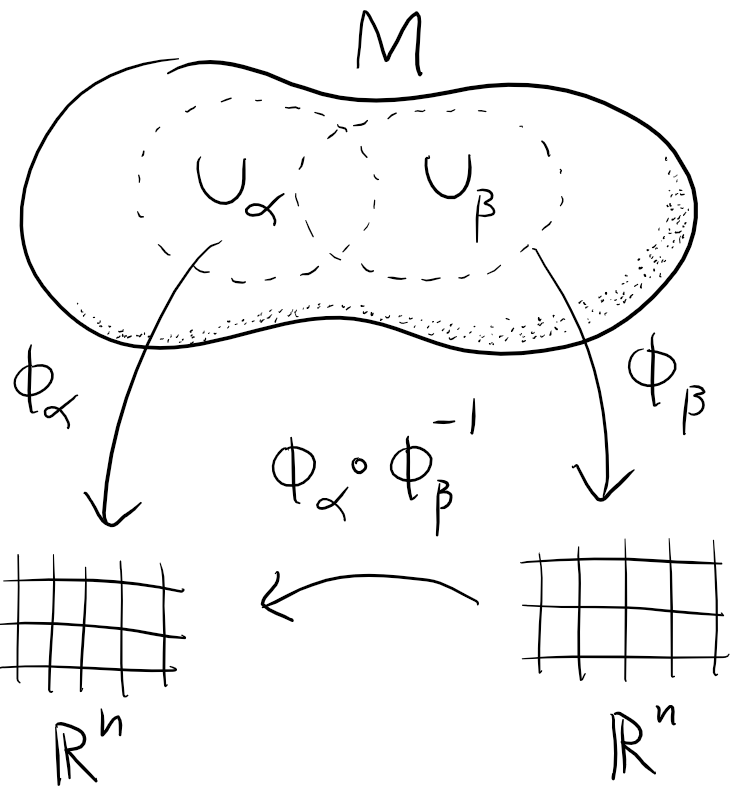
\includegraphics[width=0.35\textwidth]{img/manifold.png}
		\caption{The transition map between charts}
	\end{center}
\end{figure}
The crucial point is that the notion of differentiability from ordinary calculus applies since a transition map is a function from $\mathbb{R}^n$ to $\mathbb{R}^n$. $n$ is the \emph{dimension} of the manifold and we call $M$ an $n$-manifold for short. (We do not allow different connected components to have different dimensions.) So a differentiable manifold is in essence a space that locally looks Euclidean on which one can do calculus, but generally more than one chart is required to avoid coordinate singularities such as the poles on the Mercator projection map.

A \emph{Lie group} is a smooth manifold that has a compatible group structure i.e. group multiplication and inversion are smooth.\footnote{One can consider $C^k$ group manifolds for various $k$, but it turns out that every $C^0$ manifold with a compatible group structure can be made into a ($C^{\infty}$) Lie group in one and only one way (Hilbert's 5th problem). This is an even stronger statement than the fact from complex analysis that a complex $C^1$ function is automatically complex $C^{\infty}$.} A paradigmatic example of a Lie group is the general linear group $\gr{GL}{n,\mathbb{R}}$ of real invertible $n \times n$ matrices. It is an open subset (of $\mathbb{R}^{n^2}$) of matrices with non-zero determinant since the determinant is a polynomial and therefore continuous, and the image $\mathbb{R}\backslash \{0\}$ is open.\footnote{If $f$ is continuous, the pre-image $f^{-1}(X)$ of an open set $X$ is open.} Multiplication is linear and thus smooth, and inversion is smooth by Cramer's rule $A^{-1} = \text{adj}(A)/\det A$.

%Even thought a Lie group is topological in nature, all of its local features are captured by a single algebraic data, its Lie algebra. At each point $p$ on an $n$-manifold, $n$ orthogonal partial derivatives are linearly independent as vectors because when they act on any function $f$ on $M$,
%\begin{align}
%	(c_j \partial_j + c_k \partial_k )f = 0
%\end{align}
%if and only if $c_j=c_k=0$. Thus, they form an $n$-dimensional vector space $T_pM$ called the \emph{tangent space} at $p$. The \emph{Lie algebra} $\al{g}$ of a Lie group $G$ is the tangent space $T_eG$ at the identity together with a bilinear map $[\, , \, ]: \al{g} \times \al{g} \to \al{g}$, the \emph{Lie bracket}, which is antisymmetric $[x,y] = -[y,x]$ for any $x,y \in \al{g}$ (or equivalently $[x,x]=0$) and satisfies the Jacobi identity
%\begin{align}
%	[x,[y,z]] + [y,[x,z]] + [z,[x,y]] &= 0.
%\end{align}
%The last two properties

A Lie group $G$ may have an infinite number of generators, but it is a fact that any neighborhood of the identity element generates the component of $G$ connected to the identity. The idea of the Lie algebra is to describe $G$ by the ``linear approximation" of $G$ at the identity. Let $C^{\infty}(M)$ be the set of all smooth functions on $M$. Locally at each point $p$ on an $n$-manifold $M$, we can take partial derivatives in $n$ linearly independent directions. They are linearly independent as vectors because for every $f \in C^{\infty}(M)$ and $a \in \mathbb{R}$, if
\begin{align}
\sum_{j=1}^n a_j \partial_j f &= 0
\end{align}
then all $a_j=0$, thus they form an $n$-dimensional vector space called the \emph{tangent space} $T_p M$ at the point $p$. Globally, define a \emph{vector field} to be a linear function $X:C^{\infty}(M) \to C^{\infty}(M)$ obeying the Leibniz rule:
\begin{align}
X(fg) &= f X(g) + X(f) g
\end{align}
for every $f,g \in C^{\infty}(M)$ i.e. a \emph{derivation}. Intuitively, a vector field assigns to each point on a manifold a vector that allows us to take a derivative in that direction. Denote the set of all vector fields on $M$ by $\al{X}(M)$. Two vector fields can be composed together but the product is not a derivation. Instead $\al{X}$ can be endowed with the anticommutative product that gives another derivation, the \emph{Lie bracket}:\footnote{$C^{\infty}(M)$ is a commutative ring as functions can be multiplied together point-wise. So $\al{X}$ is a $C^{\infty}(M)$-module. The Lie bracket turns $\al{X}$ into a $C^{\infty}(M)$-algebra.}
\begin{align}
[X,Y] &= X \circ Y-Y \circ X.
\end{align}
The \emph{Jacobi identity}
\begin{align}
[X,[Y,Z]] + [Y,[Z,X]] + [Z,[X,Y]] &= 0,
\end{align}
says that the Lie bracket is a derivation with respect to itself
\begin{align}
	[X,[Y,Z]] &= [Y,[X,Z]] + [[X,Y],Z].
\end{align}
Given two smooth manifolds $M$ and $N$, and a smooth map $\varphi: M \to N$, we can construct a linear map from $\al{X}(M)$ to $\al{X}(N)$. The \emph{pushforward} $\varphi_*$ of $\varphi$ is defined to be
\begin{align}
[\varphi_*(X)](f) &\coloneqq  X[f \circ \varphi],
\end{align}
$X \in \al{X}(M)$ and $f \in C^{\infty}(N)$. When $M = G$ is a group, there is a distinct subset of vector fields whose value everywhere can be translated from the value at the identity $e$ by the pushforward of (left) group multiplication $X(g) = g_* [X(e)]$. The \emph{Lie algebra} $\text{Lie}(G)$ of a $G$ is defined to be these \emph{left-invariant vector fields} isomorphic to $T_e G$.

From the discussion above, it will come as no surprise that an abstract \emph{Lie algebra} $\al{g}$ is defined as a vector space together with a bilinear map $[\, , \, ]: \al{g} \times \al{g} \to \al{g}$, which is antisymmetric $[X,Y] = -[Y,X]$ for any $X,Y \in \al{g}$ (or equivalently $[X,X]=0$) and satisfies the Jacobi identity
\begin{align}
[X,[Y,Z]] + [Y,[Z,X]] + [Z,[X,Y]] &= 0.
\end{align}

%------------------------------------
\subsection{Matrix Lie groups}\label{ch2:matrix-group}
%------------------------------------

There is more than one possible way to define a submanifold which, in turn, affects the definition of a Lie subgroup. A smooth map $\varphi:M \to N$ is an \emph{immersion} if its pushforward $\varphi_*$ has full rank $\dim M$ for every point $p$ on $M$. An \emph{immersed submanifold} $N \subset M$ is a subset of $M$ which is itself a smooth manifold and the inclusion map $\imath: N \xhookrightarrow[]{} M$ is an immersion. A stronger notion is that of an \emph{embedded submanifold}, an immersed submanifold such that the inclusion map is a homeomorphism. An embedded submanifold inherits the topological structure from the manifold while an immersed submanifold may not. An example of the latter is the ``figure 6" map that takes an open interval to a shape with a different topology \cite{FH}:

\begin{figure}[H]\label{fig:6}
	\begin{center}
		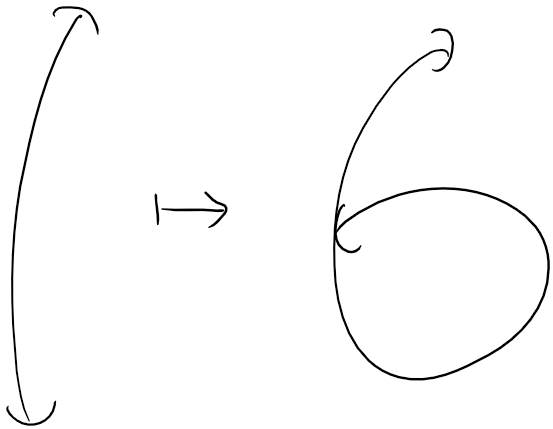
\includegraphics[width=0.35\textwidth]{img/figure-6-map.png}
		\caption{The ``figure 6" map}
	\end{center}
\end{figure}
\noindent 
Subgroups of a Lie group which are also immersed submanifolds are in one-one correspondence to Lie subalgebras of the group. Thus, one call these subgroups \emph{Lie subgroups}. Lie subgroups that are also embedded as submanifolds are not hard to come by as a result of the following theorem:
\begin{theorem}\label{thm:closed-subgroup} {\normalfont (The closed subgroup theorem) %\cite[Theorem 2.9, p.7]{Kirillov}
\cite[Theorem 20.12 p. 523]{Lee}}
	Any subgroup that is also a (topologically) closed subset \footnote{Technically, this theorem applies to discrete subgroups as any discrete group is a zero-dimensional Lie group, but we will not consider a discrete group in this context.} is a Lie subgroup which is embedded as a submanifold.
\end{theorem}
\noindent Note that the subset only needs to be closed in $G$ and not in any ambient space that $G$ is sitting in.

As an application of the theorem, since $\gr{GL}{n,\mathbb{R}}$ is a Lie group, a subgroup $G$ of $\gr{GL}{n,\mathbb{R}}$ such that any sequence of matrices in $G$ either converges in $G$ or outside $\gr{GL}{n,\mathbb{R}}$ (not invertible) is also a Lie group, called a \emph{(real) matrix Lie group}. The Lie algebra of a matrix group $G$ is the set of all matrices $X$ such that the exponential $e^X$ lands in $G$. For example the Lie algebra of $\gr{GL}{n,\mathbb{R}}$ is $\mat{n}{n}$, the set of all real $n \times n$ matrices. Let us give examples of real matrix groups that often appear in linear algebra, traditionally called the \emph{classical groups}, along with their Lie algebras, written in Fraktur.
\begin{enumerate}
	\item  The \emph{special linear group} is the connected component of matrices with determinant 1 in $\gr{GL}{n,\mathbb{R}}$.
	\begin{align}
	\gr{SL}{n,\mathbb{R}} &= \{ A \in \gr{GL}{n,\mathbb{R}} | \det A = 1 \} \\
	\al{sl}(n,\mathbb{R}) &= \{ X \in \mat{n}{n} | \Tr X = 0 \} \\
	\dim \gr{SL}{n,\mathbb{R}} &= n^2 - 1
	\end{align}
	
	\item The \emph{unitary group} is the group of matrices that preserve the Hermitian inner product $\braket{\, ,\,} :\mathbb{C}^{n} \times \mathbb{C}^{n} \to \mathbb{C}$:
	\begin{align}
		\braket{u,v} &= \sum_j u_j^* v_j.
	\end{align}
	The unitary Lie algebra is the set of all anti-Hermitian matrices.
	\begin{align}
	\gr{U}{n} &= \{ A \in \matc{n}{n} | A\dgg A = \id \} \\
	\al{u}(n) &= \{ X \in \matc{n}{n} | X\dgg  + X = 0 \} \\
	\dim \gr{U}{n} &= n^2
	\end{align}
	Despite the appearance of complex numbers, $\gr{U}{n}$ can be considered a real matrix group as $\mathbb{C}^n$ can be thought of as a real vector space $\mathbb{R}^{2n}$ of twice the dimensions.
	
	\item The \emph{special unitary group}.
	\begin{align}
	\gr{SU}{n} &= \{ A \in \gr{U}{n} | \det A = 1 \} \\
	\al{su}(n) &= \{ X \in \al{u}(n) | \Tr X = 0 \} \\
	\dim \gr{SU}{n} &= n^2 - 1
	\end{align}
	
	\item The \emph{(real) orthogonal group} $\gr{O}{n,\mathbb{R}}$ is the group of matrices that preserve the (symmetric) inner product $ g :\mathbb{R}^{n} \times \mathbb{R}^{n} \to \mathbb{R}$:
	\begin{align}
	g(u,v) &= \sum_{j=1}^{n} u_j v_j.
	\end{align}
	The connected component of matrices with determinant 1 constitutes the \emph{special orthogonal groups} $\gr{SO}{n,\mathbb{R}}$ which has the same Lie algebra, the set of all anti-symmetric matrices.
	\begin{align}
	\gr{O}{n,\mathbb{R}} &= \{ A \in \gr{GL}{n,\mathbb{R}} | A^T A = \id \} \\
	\gr{SO}{n,\mathbb{R}} &= \{ A \in \gr{O}{n,\mathbb{R}} | \det A = 1 \} \\
	\al{so}(n,\mathbb{R}) = \al{o}(n,\mathbb{R}) &= \{ X \in \mat{n}{n} | X^T + X = 0 \} \\
	\dim \gr{SO}{n,\mathbb{R}} &= \frac{n(n-1)}{2}
	\end{align}
	
	\item The (real) \emph{symplectic group} $\gr{Sp}{2n,\mathbb{R}}$ is the group of matrices that preserve the symplectic form $\omega :\mathbb{R}^{2n} \times \mathbb{R}^{2n} \to \mathbb{R}$:
	\begin{align}
	\omega(u,v) &= g(u,\Omega v) = \sum_{j=1}^{n} \left( u_j v_{n+j} - u_{n+j} v_j \right),
	\end{align}
	where
	\begin{align}
	\Omega &= \begin{pmatrix}
	{\huge 0} & \id \\
	-\id & {\huge 0}
	\end{pmatrix}.
	\end{align}
	\begin{align}
	\gr{Sp}{2n,\mathbb{R}} &= \{ A \in \gr{GL}{n,\mathbb{R}} | AJA^T = J \} \\
	\al{sp}(2n,\mathbb{R}) &= \{ A \in \mat{2n}{2n} | AJ + JA^T  = 0 \} \\
	\dim \gr{Sp}{2n,\mathbb{R}} &= n(2n+1)
	\end{align}
	A non-obvious fact, following from a Pfaffian identity \cite[p.119]{Procesi}, is that every symplectic matrix has determinant 1.
	
\end{enumerate}

$\gr{SO}{2n,\mathbb{R}}$ and $\gr{Sp}{2n,\mathbb{R}}$ are infinitesimally generated by $n$-mode quadratic fer\-mi\-on\-ic Hamiltonians and quadratic bosonic Hamiltonians, respectively.
The symmetric inner product and the symplectic form are, respectively, the real part and the imaginary part of the Hermitian inner product
\begin{align}
\braket{u,v} &= g(u,v) + i\omega(u,v).
\end{align}
(This is the local version of the K{\"a}hler structure (\autoref{app:kahler}).) Together with the fact that symplectic matrices have determinant 1, it follows that
\begin{align}\label{2-out-of-3-property}
\gr{U}{n} &\simeq \gr{SO}{2n,\mathbb{R}} \cap \gr{Sp}{2n,\mathbb{R}}.
\end{align}
This ortho-symplectic subgroup isomorphic to the unitary group is the group of particle-number-pre\-serv\-ing transformations for both bosons and fermions i.e. transformations that do not mix creation and annihilation operators.

%------------------------------------
\subsection{Representations of semisimple Lie algebras}\label{ch2:semisimple}
%------------------------------------

The theory is greatly simplified when we work over complex numbers. The \emph{complexification} $\al{g}^{\mathbb{C}} = \al{g} \oplus i\al{g}$ of a Lie algebra $\al{g}$ with the obvious Lie bracket is again a Lie algebra. An important example is $\al{gl}(n,\mathbb{C})$ which is the complexification of $\al{u}(n)$ because every complex matrix can be written as $A = B +iC$, where $B$ and $C$ are anti-Hermitian. Let us write for classical Lie algebras
\begin{align}
\al{sl}(n) &= \al{sl}(n,\mathbb{C}) = \al{u}(n)^{\mathbb{C}}, \\
\al{so}(n) &= \al{so}(n,\mathbb{C}) = \al{so}(n,\mathbb{R})^{\mathbb{C}}, \\
\al{sp}(n) &= \al{sp}(2n,\mathbb{C}) = \al{sp}(2n,\mathbb{R})^{\mathbb{C}}.
\end{align}

An \emph{ideal} $\al{k}$ of $\al{g}$ is a vector subspace
that absorbs every element of $\al{g}$ into itself: $[\al{k},\al{g}] \subset \al{k}$.
An ideal is a Lie subalgebra of $\al{g}$ and the Lie algebra of a normal subgroup of $G$. If $G$ has a nontrivial normal subgroup $K$, then to study $G$ we can study a simpler group $G/K$ through its Lie algebra $\al{g/k}$. A Lie algebra is \emph{simple} if it is not abelian (not every Lie bracket is zero) and has no nontrivial ideal. (The non-abelianity is there to make every simple Lie algebra semisimple, but it is a rather trivial condition to rule out $\al{u}(1)$, the only abelian Lie algebra which has no nontrivial ideal.) $\al{sl}(n)$ for $n \ge 2$, $\al{so}(n)$ for $n=3$ and $n \ge 5$, and $\al{sp}(n)$ are simple Lie algebras.

A \emph{representation} of a Lie algebra $\al{g}$ is a Lie algebra homomorphism $\pi: \al{g} \to \text{End}(V)$ i.e. a linear map respecting the Lie bracket:
\begin{align}
\pi([X,Y]) &= [\pi(X),\pi(Y)]
\end{align}
for all $X,Y \in \al{g}$. The \emph{adjoint representation} of $\al{g}$ is the Lie algebra homomorphism
\begin{align}
\text{ad}: \al{g} &\to \text{End}\al{g}, \\
\adrep X (Y) &= [X,Y].
\end{align}
It is the pushforward of the adjoint representation of its Lie group $G$ on the Lie algebra:
\begin{align}
\Adrep g (X) &= gXg^{-1}.
\end{align}
The two are related by the well known identity
\begin{align}
	e^Y X e^{-Y} &= e^{\adrep{Y}} X.
\end{align}
A bilinear form $\braket{\, , \,}$ is invariant with respect to the adjoint action if
\begin{align}
\braket{ \Adrep g (Y), \Adrep g (Z)} &= \braket{Y,Z}
\end{align}
or equivalently, by setting $g=e^{tX}$ and differentiating with respect to $t$
at the identity element,
\begin{align}
\braket{\adrep X (Y),Z} + \braket{Y,\adrep X (Z)} &= 0.
\end{align}
Any representation of a Lie algebra gives an invariant bilinear form $\braket{X,Y} =\\ \Tr [\pi(X) \pi(Y)]$. When $\pi$ is the adjoint representation, we have the \emph{Killing form}
\begin{align}\label{def:killing-form}
\kil{X}{Y} &\coloneqq \Tr (\adrep X \adrep Y),
\end{align}
which turns out to be proportional to $\Tr (XY)$ when the group is simple.
The Killing form of a compact real Lie group $G$ is negative semidefinite. To show this, we use the fact that every finite-dimensional representation of a compact group is unitary, thus every representation of $G$ sits inside $\al{u}(n) = \{ X \in \matc{n}{n} | X\dgg  + X = 0 \}$. Therefore, $\Tr (X^2) = - \Tr(XX\dgg ) = -\sum_{j,k} |X_{jk}|^2 \le 0$.

Over $\mathbb{C}$, a \emph{semisimple Lie algebra} $\al{g}$ can be defined by the following equivalent conditions: \cite[p.89]{Procesi}
\begin{enumerate}
	\item $\al{g}$ has no abelian ideal.
	\item  The Killing form on $\al{g}$ is non-degenerate. \emph{(Cartan's criteria for semisimplicity)}
	\item $\al{g} = \bigoplus_j \al{g}_j$ is a direct sum of simple Lie algebras $\al{g}_j$ mutually orthogonal with respect to the Killing form.
\end{enumerate}
A Lie group $G$ is simple or semisimple if its Lie algebra is simple or semisimple respectively. Given a complex Lie algebra $\al{g}$, there is a real Lie subalgebra $\al{k}$ whose complexification is $\al{g}$. If, moreover, $\al{g}$ is semisimple, then there is a compact, simply-connected group $K$ with $\al{k}^{\mathbb{C}} = \al{g}$, and representations of $\al{g}$, $\al{k}$, and $K$ can be studied interchangeably \cite[p.112]{Kirillov}.

The unique compact, simply-connected group associated with the classical group $\gr{SO}{n,\mathbb{R}}$ is its universal covering group, the \emph{spin group} $\gr{Spin}{n}$.\footnote{$\gr{SO}{n,\mathbb{R}}$ is not simply-connected. For instance, the rotation group $\gr{SO}{3,\mathbb{R}}$ is topologically a three-dimensional ball with antipodal points identified: the two angles parametrize the axis of rotation and the radius parametrizes the angle of rotation. Antipodal points are $\pi$ and $-\pi$ rotations. Any nontrivial path between antipodal points is a loop that cannot be shrunk to a single point.}
That is, $\gr{Spin}{n}$ is a unique compact, simply-connected Lie group such that there exists a surjective (onto) Lie group homomorphism
\begin{align}\label{def:spin-group}
	\gr{Spin}{n} \twoheadrightarrow \gr{SO}{n,\mathbb{R}}.
\end{align}
It is also a double cover of $\gr{SO}{n,\mathbb{R}}$, meaning that there is a representation of $\gr{Spin}{n}$ which is a representation of $\gr{SO}{n,\mathbb{R}}$ only up to a sign (projective representation), called a \emph{spinor representation}.

%------------------------------------
\subsection{Roots and weights}\label{ch2:root}
%------------------------------------

The structure theory of complex semisimple Lie algebras mimics and generalizes the $\al{su}(2)$ case familiar to every physicist from the quantum theory of angular momentum, which we briefly remind the reader here. Consider the Pauli matrices:
\begin{align}
X & =\left(\begin{array}{cc}
0 & 1\\
1 & 0
\end{array}\right),&
Y & =\left(\begin{array}{cc}
0 & -i\\
i & 0
\end{array}\right),&
Z & =\left(\begin{array}{cc}
1 & 0\\
0 & -1
\end{array}\right).
\end{align}
$\al{su}(2)$ is a real Lie algebra whose basis can be chosen to be $\{ iX,iY,iZ \}$,
\begin{align}
[iX,iY] &= -2iZ,&
[iY,iZ] &= -2iX,&
[iZ,iX] &= -2iY.
\end{align}
Physicists' version of the commutation relations of $\al{su}(2)$ are in fact those of $\al{sl}(2) = \al{su}(2)^{\mathbb{C}}$:
\begin{align}
[X,Y] & =2iZ,&
[Y,Z] & =2iX,&
[Z,X] & =2iY,
\end{align}
In the basis
\begin{align}
H & =Z,&
E_{\pm} & =\frac{X \pm iY}{2}
\end{align}
one has the commutation relations
\begin{align}
[H,E_{\pm}] &= \pm 2E_{\pm},&
[E_+,E_-] & =H.
\end{align}
From this, one derives that there is exactly one distinct irrep in each dimension $\lambda+1$---referred to in the physics jargon as the spin-$\lambda/2$ representation---and these are all the finite-dimensional irreps of $\gr{sl}{2}$. Each irrep $(\pi_{\lambda},V_{\lambda})$ decomposes into mutually orthogonal eigenvectors of $\pi_j(H)$.
\begin{align}
\pi_{\lambda}(H) \ket{\lambda,\mu} &= \mu \ket{\lambda,\mu}.
\end{align}
The integral eigenvalues $\mu$ are \emph{weights} and the eigenvectors are \emph{weight vectors}. $V_{\lambda}$ can be constructed by recursively applying the lowering operator $E_-$ starting from the highest weight vector:
\begin{align}
\pi_{\lambda}(E_+) \ket{\lambda,\lambda} &= 0,
\end{align}
making use of the relation
\begin{align}
\pi_{\lambda}(H) \pi_{\lambda}(E_-) \ket{\lambda,\mu} &= (\mu - 2)\pi_{\lambda}(E_-) \ket{\lambda,\mu} %\\
%\pi_{\lambda}(H) \pi_{\lambda}(F) \ket{\lambda,\mu} &= (\lambda - 2)\pi_{\lambda}(F) \ket{\lambda,\mu}.
\end{align}

For general complex semisimple Lie algebras, $H$ generalizes to a \emph{Cartan subalgebra}, a maximal abelian subalgebra $\al{h} \subset \al{g}$ such that $\adrep H$ is diagonalizable for every $H \in \al{h}$ \cite[Proposition 2.13, p.136]{Knapp}. (Beware that this definition is only valid for semisimple Lie algebras.)
Every complex semisimple Lie algebra of $G$ has a Cartan subalgebra, and a Cartan subalgebra is the complexified Lie algebra of some maximal torus in $G$. A Cartan subalgebra is not unique, but all Cartan subalgebras are conjugated, thus have the same dimension called the \emph{rank} of the Lie algebra.

The most important result about semisimple Lie algebras---much more important than the definition of semisimple Lie algebras itself \cite{Kirillov}---is the \emph{root space decomposition} of the adjoint representation $\al{g}$. Since $\al{h}$ is abelian, all $\adrep H$ are simultaneously diagonalizable, decomposing $\al{g}$ into a direct sum
\begin{align}
\al{g} &\stackrel{\al{g}}{\simeq} \al{h} \oplus \bigoplus_{\alpha \in \mathcal{R}}\al{g}_{\alpha},
\end{align}
where
\begin{align}
	 \al{g}_{\alpha} &= \{ E_{\alpha} \mid [H,E_{\alpha}] = \alpha(H) E_{\alpha}, \forall H \in \al{h} \}
\end{align}
is called a \emph{root space}. Each \emph{root} $\alpha \in \al{h}^* - \{0\}$ (linear non-zero forms on $\al{h}$) corresponds to an eigenvalue $\alpha(H)$ and a \emph{root vector} $E_{\alpha}$. The finite set $\mathcal{R}$ of roots is called the \emph{root system}. Roots are special cases of weights in the adjoint representation. Roots and root spaces have the following properties:
\begin{enumerate}
	
	\item Every $\al{g}_{\alpha}$ is one-dimensional.
	
	\item\label{root-space-orthogonality} Writing $\al{g}_0 = \al{h}$, taking a commutator is equivalent to adding roots:
	\begin{align}
	[\al{g}_{\alpha} , \al{g}_{\beta}] \subset \al{g}_{\alpha+\beta}.
	\end{align}
	Furthermore, $\al{g}_{\alpha}$ and $\al{g}_{\beta}$ are orthogonal with respect to the Killing form whenever $\alpha + \beta \neq 0$ (whereas $\al{g}_{\alpha}$ and $\al{g}_{-\alpha}$ are never orthogonal).
	
	\item\label{root-span} $\mathcal{R}$ spans $\al{h}^*$.
	
	\item\label{positive-root} For every $\alpha \in \mathcal{R}$, the only non-zero multiples of $\alpha$ that are in $\mathcal{R}$ are $\pm \alpha$.
	
\end{enumerate}
%To prove \ref{root-space-orthogonality}, note that
%\begin{align}
%	(\adrep E_{\alpha} \adrep E_{\beta}) E_{\gamma} &= E_{(\alpha + \beta) + \gamma}.
%\end{align}
%$\adrep E_{\alpha} \adrep E_{\beta}$
%therefore has no diagonal element, making the Killing form vanishes.
A consequence of property \ref{root-space-orthogonality} is that the Killing form restricted to $\al{h}$ is non-degenerate and thus can be used to identify $\al{h}$ and $\al{h}^*$. Even though there is \emph{a priori} no preferred basis for $\al{h}$, there is a preferred basis in $\al{h}^*$ consisting of the roots. In particular, the Killing form associates to each $\alpha \in \al{h}^*$ %and $E_{\alpha} \in \al{g}_{\alpha}$
, $H_{\alpha} \in \al{h}$ via
\begin{align}
\kil{H_{\alpha}}{H} &= \alpha(H).
\end{align}
To keep the notation tidy, we write the inner product of two roots as
\begin{align}
\braket{\alpha,\beta} &\coloneqq \kil{H_{\alpha}}{H_{\beta}} = \alpha(H_{\beta}) = \beta(H_{\alpha}).
\end{align}
The number $\braket{\alpha,\alpha}$ is called the \emph{length} of the root $\alpha$. The \emph{Cartan basis} is
\begin{align}
[H,E_{\alpha}] &= \alpha(H) E_{\alpha}, \\
[E_{\alpha}, E_{\beta}] &=
\begin{cases}
N_{\alpha \beta} E_{\alpha + \beta}, & \alpha + \beta \neq 0, \alpha + \beta \in \mathcal{R}, \\
\braket{\alpha,-\alpha} H_{\alpha}, & \alpha + \beta = 0,
\end{cases}
\end{align}
where the last commutator follows directly from the invariance of the Killing form $\kil{[E_{\alpha}, E_{-\alpha}]}{H} = \kil{E_{\alpha}}{[E_{-\alpha}, H]}$ and $[H,[E_{\alpha},E_{-\alpha}]]=0$.

Simple roots are introduced to provide a succinct description of complex semisimple Lie algebras. From properties \ref{root-span} and \ref{positive-root} of a root system, if we make an arbitrary choice of which of the roots $\pm \alpha$ to call \emph{positive}, then the set of positive roots $\mathcal{R}_+$ spans $\al{h}^*$. The collection $\Delta$ of \emph{positive simple roots}, positive roots that cannot be written as nontrivial linear combinations of other roots, forms a basis for $\al{h}^*$.\footnote{Each positive simple root corresponds to a copy of $\al{sl}(2)$. To see this, rescale $E_{\alpha}$ and $E_{-\alpha}$ so that $\kil{E'_{\alpha}}{E'_{-\alpha}} = 2/\braket{\alpha,\alpha}$ and set $H'_{\alpha} = 2H_{\alpha}/\braket{\alpha,\alpha}$. Then
	\begin{align}
	[H',E'_{\pm}] &= \pm 2E'_{\pm},&
	[E'_+,E'_-] &= H',
	\end{align}
	is the basis of a subalgebra isomorphic to $\al{sl}(2)$.}  The \emph{Cartan matrix} is defined to be the matrix of integers
\begin{align}
A_{jk} &\coloneqq \frac{2\braket{\alpha_k,\alpha_j}}{\braket{\alpha_j,\alpha_j}}.
\end{align}
The Cartan matrix depends on the choice of positive simple roots $\Delta$ but different choices give Cartan matrices that are conjugate to each other by a permutation matrix. A unique \emph{Dynkin diagram} can be associated with equivalent Cartan matrices by the following algorithm:
\begin{enumerate}
	\item Draw a vertex for each simple root $\alpha_j$.
	\item Connect vertices $\alpha_j$ and $\alpha_k$ by $A_{jk}A_{kj}$ edges.
	\item Draw an arrow pointing from a longer root to a shorter root. (The arrow's head is the greater-than sign $>$.)
\end{enumerate}
The classical Lie algebras introduced earlier are all simple. In fact, they exhaust the list of infinite families of finite-dimensional, complex semisimple Lie algebras parametrized by the number of positive roots $n$, which is also the same as the rank. Belows are the Dynkin diagrams, built from right to left, of the classical groups.
\begin{center}
	\begin{tikzpicture}
	
	\draw (0,0) -- (1,0);
	\draw (2,0) -- (2.7,0);
	\draw (1,0) -- (2,0);
	\draw (3.3, 0) -- (4,0);
	\draw (4,0) -- (5,0);
	
	\draw[fill=white] (0,0) circle(.1);
	\draw[fill=white] (1,0) circle(.1);
	\draw[fill=white] (2,0) circle(.1);
	\draw[fill=white] (4,0) circle(.1);
	\draw[fill=white] (5,0) circle(.1);
	
	\node at (3,0) {$\cdots$};
	\node at (-2.15,0) {$A_n = \al{sl}(n+1)$};
	
	\end{tikzpicture}
	
	\begin{tikzpicture}
	
	\draw (0,0) -- (2.7,0);
	\draw (3.3, 0) -- (4,0);
	\draw (4,0.1) -- (5,0.1);
	\draw (4,-0.1) -- (5,-0.1);
	\draw (4.4,0.2) -- (4.6,0);
	\draw (4.4,-0.2) -- (4.6,0);
	
	\draw[fill=white] (0,0) circle(.1);
	\draw[fill=white] (1,0) circle(.1);
	\draw[fill=white] (2,0) circle(.1);
	\draw[fill=white] (4,0) circle(.1);
	\draw[fill=white] (5,0) circle(.1);
	
	\node at (3,0) {$\cdots$};
	\node at (-2,0) {$B_n = \al{so}(2n+1)$};
	
	\end{tikzpicture}
	
	\begin{tikzpicture}
	
	\draw (0,0) -- (2.7,0);
	\draw (3.3, 0) -- (4,0);
	\draw (4,0.1) -- (5,0.1);
	\draw (4,-0.1) -- (5,-0.1);
	\draw (4.4,0) -- (4.6,0.2);
	\draw (4.4,0) -- (4.6,-0.2);
	
	\draw[fill=white] (0,0) circle(.1);
	\draw[fill=white] (1,0) circle(.1);
	\draw[fill=white] (2,0) circle(.1);
	\draw[fill=white] (4,0) circle(.1);
	\draw[fill=white] (5,0) circle(.1);
	
	\node at (3,0) {$\cdots$};
	\node at (-2.45,0) {$C_n = \al{sp}(n)$};
	
	\end{tikzpicture}
	
	\begin{tikzpicture}
	
	\draw (0,0) -- (2.7,0);
	\draw (3.3, 0) -- (4,0);
	\draw (4,0) -- (5,-.5);
	\draw (4,0) -- (5,.5);
	
	\draw[fill=white] (0,0) circle(.1);
	\draw[fill=white] (1,0) circle(.1);
	\draw[fill=white] (2,0) circle(.1);
	\draw[fill=white] (4,0) circle(.1);
	\draw[fill=white] (5,-.5) circle(.1);
	\draw[fill=white] (5,.5) circle(.1);
	
	\node at (3,0) {$\cdots$};
	\node at (-2.35,0) {$D_n = \al{so}(2n)$};
	
	\end{tikzpicture}
\end{center}


\noindent That is, $ \ran \al{sl}(n) = n-1$, $\ran \al{so}(n) = \lfloor n/2 \rfloor$, and $\ran \al{sp}(n) = n$. We also notice from the diagrams isomorphisms of low-dimensional Lie algebras: $\al{su}(2) \allowbreak = \al{so}(3) = \al{sp}(1)$, $\al{so}(4) = \al{sl}(2) \oplus \al{sl}(2)$, $\al{so}(5) = \al{sp}(2)$, and $\al{su}(4) = \al{so}(6)$. ($\al{u}(1) = \al{so}(2)$ are abelian, thus not simple.)

Every representation of a complex semisimple Lie algebra can be characterized by its highest weight. In a representation $(\pi,V)$, a simultaneous eigenvector of the restriction of $\pi$ to the Cartan subalgebra $\ket{v} \in V$ is called a vector of \emph{weight} $\lambda$ if
\begin{align}
\pi(H) \ket{v} = \lambda(H) \ket{v}.
\end{align}
$V$ decomposes into (not necessarily one-dimensional) \emph{weight spaces}:
\begin{align}
V &\stackrel{\al{g}}{\simeq}  \bigoplus_{\lambda}V_{\lambda},
\end{align}
where
\begin{align}
	V_{\lambda}
	&\coloneqq \bigoplus_{\lambda} \{ \ket{v} \in V \big| \pi(H) \ket{v} = \lambda(H) \ket{v}, \forall H \in \al{h} \}.
\end{align}
The weights can be given a partial ordering: $\lambda \succeq \mu$ if and only if the difference $\lambda - \mu$ is a positive linear combination of positive simple roots. A weight then is a \emph{highest weight} of $\pi$ if $\lambda \succ \mu$ for every weight $\mu$ of $\pi$. A weight $\lambda$ is said to be \emph{integral} if $2\braket{\lambda,\alpha}/\braket{\alpha,\alpha}$ is an integer for every positive simple root $\alpha \in \Delta$. If the integer is in addition positive, the weight is said to be \emph{dominant integral}. It turns out that every weight is integral. The \emph{highest weight theorem} guarantees that each and every dominant integral weight $\lambda$ gives distinct finite dimensional irreps of $\al{g}$ with the highest weight $\lambda$ and every finite dimensional irrep of $\al{g}$ arises in this way. One then applies negative simple roots to the highest weight vector to generate an orthonormal basis for each irrep.

%------------------------------------
\subsection{Realizations of classical Lie algebras by creation and annihilation operators}\label{ch2:physics-realization}
%------------------------------------

$\al{gl}(n)$ can be explicitly realized by operators quadratic and linear in either the bosonic or fermionic creation and annihilation operators \cite[Chapter 9 and 10]{iachello}. Since matrix Lie algebras are Lie subalgebras of $\al{gl}(n)$, all matrix Lie algebras have bosonic and fermionic realizations. (The bosonic realizations of the classical Lie algebras are summarized in \cite[\S 10.4, p. 309]{Barut}. Well known is the bosonic realization of $\al{gl}(n)$ called the Schwinger representation \cite{Schwinger}.) To prove the realizations, we only need to verify that the appropriate bosonic or fermionic operators are eigenvectors of the adjoint representation of a Cartan subalgebra with the eigenvalues as the roots. The roots of the classical Lie algebras can be found on a case-by-case basis \cite{FH}.

The fermionic creation and annihilation operators for $n$ modes are defined by the canonical anticommutation relation
\begin{align}
\{a_j,a_k\dgg \} &= \delta_{jk}\id, &
\{a_j,a_k\}&=0.
\end{align}
To simplify the notations, let us define
\begin{align}
E^j{}_k &\coloneqq a_j\dgg a_k - \frac{1}{2}\delta_{jk}\id, &
E^{jk} 	&\coloneqq a_j\dgg a_k\dgg, &
E_{jk} &\coloneqq a_j a_k.
\end{align}
Then
\begin{align}
	E^j{}_k{}\dgg &= E^k{}_j, &
	E^{jk \dagger} &= E_{kj}, &
	E_{jk} &= -E_{kj},
\end{align}
and
\begin{equation*}
	\noindent\begin{minipage}[t]{.5\textwidth}
		\begin{align}
		[a_j,a_k] &= 2E_{jk}, \\
		[a_j\dgg,a_k] &= 2E^j{}_k, \\
		[a_j,E^k{}_l] &= \delta_{jk} a_l, \label{so(2n+1)-commutation-relations} \\
		[a_j,E^{kl}] &= \delta_{jk} a_l\dgg - \delta_{jl}a_k\dgg, \\
		[a_j,E_{kl}] &= 0,
		\end{align}
	\end{minipage}%
	\begin{minipage}[t]{.5\textwidth}
		\begin{align}
		[E^j{}_k,E^l{}_m] &= \delta_{lk}E^j{}_m - \delta_{jm}E^l{}_k, \label{u(n)-commutation-relations} \\
		[E^j{}_k,E_{lm}] &= \delta_{jm}E_{kl} - \delta_{jl}E_{km}, \\
		\begin{split}
			[E^{jk},E_{lm}] &= \delta_{jm}E^k{}_l + \delta_{kl}E^j{}_m \\
			&- \delta_{jl}E^k{}_m - \delta_{km}E^j{}_l,
		\end{split} \\
		[E_{jk},E_{lm}] &= 0,
		\end{align}
	\end{minipage} \nonumber
\end{equation*}

Now we are ready to give the fermionic realizations of the orthogonal Lie algebras and of $\al{gl}(n)$, which for our purpose, is thought of as a subalgebra of the orthogonal ones.

%------------------------------------
\subsubsection{$\text{B}_n = \al{so}(2n+1)$}
%------------------------------------
$\al{so}(2n+1)$ can be realized by all quadratic and linear fermionic operators.
The $n$-dimensional Cartan subalgebra $\al{h}$ can be chosen to be the span of $\{E^j{}_j\}$.
Let $e_j$ be a linear form such that $e_j (E^k{}_k) = \delta_{jk}$. The roots are
\begin{align}
	R &= \{ e_j \pm e_k, -(e_j \pm e_k), \pm e_j |j \neq k \}.
\end{align}
Positive simple roots can be chosen to be
\begin{align}
	\Delta &= \{ -e_1, e_1 - e_2, \dots, e_{n-1} - e_n \}.
\end{align}
Using the commutation relations eq. \eqref{so(2n+1)-commutation-relations} and eq. \eqref{u(n)-commutation-relations},
\begin{align}
[E^j{}_j, a_k] &= -[a_k, E^j{_j}]\dgg = -\delta_{jk} a_k = -e_k(E^j{}_j) a_k, \\
[E^j{}_j, E^k{}_l] &= \delta_{jk} E^j{}_l - \delta_{jl} E^k{}_j = (e_k - e_l) (E^j{}_j) E^k{}_l.
\end{align}
Therefore, we have
\begin{align}
	\Delta = \{ a_1, a_1\dgg a_2, \dots, a_{n-1}\dgg a_n \}.
\end{align}
Via the Killing form, the root $-e_j$ is associated, up to a scalar multiple, with $H_{\alpha_j} = -E^j{}_j$. Similarly, the roots $\alpha_j = e_{j-1} - e_j$ are associated with $H_{\alpha_j} = E^{j-1}{}_{j-1} - E^j{}_j$, up to the same scalar multiple. One can then calculate the inner product $\braket{\alpha_j,\alpha_k} = \kil{H_{\alpha_j}}{H_{\alpha_k}}$ between all pair of roots to obtain the Dynkin diagram:
\begin{center}
	\begin{tikzpicture}
	
	\draw (0.5,0.1) -- (1.5,0.1);
	\draw (0.5,-0.1) -- (1.5,-0.1);
	\draw (0.9,0) -- (1.1,0.2);
	\draw (0.9,0) -- (1.1,-0.2);
	\draw (2.5,0) -- (3.1,0);
	\draw (3.8,0) -- (4.7,0);
	\draw (5.3,0) -- (6,0);
	
	\draw[fill=white] (0,0) circle(.5);
	\draw[fill=white] (2,0) circle(.5);
	\draw[fill=white] (3.5,0) circle(.5);
	\draw[fill=white] (6.5,0) circle(.5);
	
	\node at (5.05,0) {$\cdots$};
	\node at (0,0) {$a_1$};
	\node at (2,0) {$a\dgg_1 a_2$};
	\node at (3.5,0) {$a\dgg_2 a_3$};
	\node at (6.5,0) {\scriptsize $a_{\!n\!-\!1}\!\dgg a_n$};
	\end{tikzpicture}
\end{center}

%------------------------------------
\subsubsection{$\text{D}_n = \al{so}(2n)$}
%------------------------------------

$\al{so}(2n)$ is a subalgebra of $\al{so}(2n+1)$ consisting of all quadratic fermionic operators. The Cartan subalgebra remains the same as $\al{so}(2n+1)$ (though $H_{\alpha_j}$ changes depending on the roots). We no longer have the linear term, so the roots and positive simple roots are
\begin{align}
R &= \{ e_j \pm e_k, -(e_j \pm e_k) |j \neq k \}, \\
\Delta &= \{-(e_1 + e_2), e_1 - e_2, \dots, e_{n-1} - e_n \},
\end{align}
Since
\begin{align}
	[E^j{}_j, E_{kl}] &= \delta_{jl} E_{jk} - \delta_{jk} E_{jl}
	= - \delta_{jl} E_{kl} - \delta_{jk} E_{kl}  \nonumber \\
	&= -(e_k + e_l) (E^j{}_j) E_{kl},
\end{align}
the positive simple roots are
\begin{align}
\Delta &= \{a_1a_2, a_1\dgg a_2, \dots, a_{n-1}\dgg a_n \},
\end{align}
and the Dynkin diagram is
\begin{center}
	\begin{tikzpicture}
	
	\draw (0.3,-1) -- (1,-0.3);
	\draw (0.3,1) -- (1,0.3);
	\draw (1,0) -- (2.7,0);
	\draw (3,0) -- (4,0);
	\draw (4.6,0) -- (5.5,0);
	
	\draw[fill=white] (0,-1.3) circle(.5);
	\draw[fill=white] (0,1.3) circle(.5);
	\draw[fill=white] (1.3,0) circle(.5);
	\draw[fill=white] (2.8,0) circle(.5);
	\draw[fill=white] (5.8,0) circle(.5);
	
	\node at (4.35,0) {$\cdots$};
	\node at (0,-1.3) {$a\dgg_1 a_2$};
	\node at (0,1.3) {$a_1 a_2$};
	\node at (1.3,0) {$a\dgg_2 a_3$};
	\node at (2.8,0) {$a\dgg_3 a_4$};
	\node at (5.8,0) {\scriptsize $a\dgg_{\!n\!-\!1}\! a_n$};
	\end{tikzpicture}
\end{center}

%------------------------------------
\subsubsection{$\text{A}_n = \al{sl}(n+1)$}
%------------------------------------

By eq. \eqref{u(n)-commutation-relations}, $\{ E^j{}_k \}$ is a subalgebra of $\al{so}(2n)$ having the root structure isomorphic to that of $\al{gl}(n) = \al{sl}(n) \oplus \al{u}(1)$, where the $\al{u}(1)$ is the total number operator $\sum_j E^j{}_j$. Consider only the simple part $\al{sl}(n)$. The Cartan subalgebra remains the same as that of the orthogonal Lie algebras. The roots and positive simple roots are
\begin{align}
	R &= \{ e_j - e_k |j \neq k \}, \\
	\Delta &= \{ e_j - e_k |j < k \}.
\end{align}
The ``two-mode squeezing" $a_j a_k$ is removed from the roots:
\begin{align}
	\Delta &= \{ a_1\dgg a_2, \dots, a_{n-1}\dgg a_n \}
\end{align}
\begin{center}
	\begin{tikzpicture}
	
	\draw (0,0) -- (2.7,0);
	\draw (3.3, 0) -- (4,0);
	
	\draw[fill=white] (0,0) circle(.5);
	\draw[fill=white] (1.5,0) circle(.5);
	\draw[fill=white] (4.5,0) circle(.5);
	
	\node at (3,0) {$\cdots$};
	\node at (0,0) {$a\dgg_1 a_2$};
	\node at (1.5,0) {$a\dgg_2 a_3$};
	\node at (4.5,0) {\scriptsize $a\dgg_{\!n\!-\!1}\! a_n$};
	\end{tikzpicture}
\end{center}

%------------------------------------
\subsubsection{$\text{C}_n = \al{sp}(n)$}
%------------------------------------

We do not use the root system of the symplectic Lie algebra anywhere in this dissertation, but note that the bosonic realization
\begin{align}
	[b_j,b_k\dgg] &= \delta_{jk}\id.
\end{align}
of positive simple roots of $\al{sp}(n)$:
\begin{align}
	\Delta &= \{-2e_1, e_1 - e_2, \dots, e_{n-1} - e_n \} \\
	&= \Bigl\{ \frac{b_1^2}{2} ,b_1\dgg b_2, \dots, b_{n-1}\dgg b_n \Bigr\}
\end{align}
	\begin{center}
		\begin{tikzpicture}
		
		\draw (0.5,0.1) -- (1.5,0.1);
		\draw (0.5,-0.1) -- (1.5,-0.1);
		\draw (1.1,0) -- (0.9,0.2);
		\draw (1.1,0) -- (0.9,-0.2);
		\draw (2.5,0) -- (3.1,0);
		\draw (3.8,0) -- (4.7,0);
		\draw (5.3,0) -- (6,0);
		
		\draw[fill=white] (0,0) circle(.5);
		\draw[fill=white] (2,0) circle(.5);
		\draw[fill=white] (3.5,0) circle(.5);
		\draw[fill=white] (6.5,0) circle(.5);
		
		\node at (5.05,0) {$\cdots$};
		\node at (0,0) {\large $\frac{b_1^2}{2}$};
		\node at (2,0) {$b\dgg_1 b_2$};
		\node at (3.5,0) {$b\dgg_2 b_3$};
		\node at (6.5,0) {\scriptsize $b_{\!n\!-\!1}\!\dgg b_n$};
		\end{tikzpicture}
	\end{center}
look very similar to those of $\al{so}(2n+1)$ except that the two-mode squeezing is replaced by a single-mode squeezing.

%------------------------------------
\section{Harmonic analysis on multiplicity-free spaces}\label{ch2:gelfand}
%------------------------------------

Traditional Fourier analysis on the real line $\mathbb{R}$ or the circle $U(1)$ is the multiplicity-free decomposition of the regular representation of an abelian group. A simple characterization of the multiplicity-free property for the representation $L^2(G/K)$ of a homogeneous space $G/K$ can be given in terms of Frobenius reciprocity. Since $L^2(G/K)$ is the representation $\ind{\mathbb{C}}{K}{G}$ induced from the trivial representation, $L^2(G/K)$ is multiplicity-free if and only if the trivial irrep of $K$ appears at most once in any irrep $V_{\lambda}$,
\begin{align}
\dim \text{Hom}_G ( V_{\lambda}, L^2(G/K) ) = \dim \text{Hom}_K (\text{Res} V_{\lambda}, \mathbb{C}) \le 1.
\end{align}

Gelfand found that $L^2(G/K)$ is multiplicity-free if and only if the space of $K$-bi-invariant functions $L^1(K\backslash G/K)$ is commutative with respect to convolution product \cite{gelfand1950spherical}.\footnote{$L^1(K\backslash G/K)$ turns out to be the space of intertwiners $\text{End}_G(L^2(G/K))$, the analogue of the \emph{Hecke algebra} for finite groups.} Such a pair $(G,K)$ is called a \emph{Gelfand pair}. We will also call the coset space $G/K$ a \emph{multiplicity-free space} if $(G,K)$ is a Gelfand pair.
%\footnote{Multiplicity-free spaces are also called \emph{commutative spaces} because of Gelfand's criterion \cite{wolf2007harmonic}, but we will not use that term since it can be confused with the term (non-)commutative \emph{phase} space.} 
The notion of a \emph{(zonal) spherical function} of an irrep $(\rep_{\lambda},V)$ makes sense on a multiplicity-free space $G/K$. It is the matrix element of $\rep_{\lambda}$ of the $K$-invariant vector in $V$, the unique trivial irrep of $K$ appearing in $V$, and they form an orthogonal basis for $L^1(K\backslash G/K)$ \cite[\S 17.3]{Vilenkin3}.

%------------------------------------
\subsection{Symmetric spaces and $KAK$ decomposition}\label{ch2:kak}
%------------------------------------

Most relevant to us is the fact that fermionic phase spaces $\homsp{SO}{2n}{U}{n}$ and $\homsp{SO}{2n+1}{U}{n}$ are multiplicity-free \cite[and references therein]{wolf2007harmonic}, and in principle, the $K$-invariant vectors are the only thing we need to construct their corresponding quasi-probability representations (\autoref{ch3:construction}). Especially, $\homsp{SO}{2n}{U}{n}$ has a special symmetry property that implies the multiplicity-free property. Let $G$ be a Lie group with a Lie algebra $\al{g}$. A nontrivial involutive Lie algebra automorphism (homomorphism onto itself) $\theta$,
\begin{align}
\theta^2 &= \id,
\end{align}
called a \emph{Cartan involution} is diagonalizable and splits $\al{g}$ into the $+1$ and $-1$ ei\-gen\-spaces $\al{k}$ and $\al{p}$ respectively. Equivalently, these subspaces obey the defining commutation relations 
\begin{align}
[\al{k},\al{k}] &\subset \al{k}, \\
[\al{k},\al{p}] &\subset \al{p}, \label{reductive} \\
[\al{p},\al{p}] &\subset \al{k}. \label{symmetric}
\end{align}
Such a pair $(G,K)$ is called a \emph{symmetric pair}, and $G/K$ is called a \emph{symmetric space} \cite{Helgason}.
We directly see from the fermionic commutation relations that $\homsp{SO}{2n}{U}{n}$ is a symmetric space while $\homsp{SO}{2n+1}{U}{n}$ is not. The multiplicity-free property can be proved directly from the existence of an involution using the Gelfand's criterion \cite[pp.36-37]{Gangolli} or from the $KAK$ decomposition below.

For $G$ non-compact semisimple, the Cartan involution leads to the \emph{Cartan decomposition}, which is a generalization of the polar decomposition for invertible matrices when $G/K = \homsp{GL}{n,\mathbb{R}}{O}{n,\mathbb{R}}$. It can be proved that the bilinear form defined by the involution
\begin{align}
	\kil{X}{\theta Y}
\end{align}
is negative definite \cite{Knapp}. Thus the Killing form is negative definite on $K$ and positive definite on $P$, showing that $K$ is a maximal compact subgroup of $G$. $G$ has the Cartan decomposition at the Lie algebra level $\al{g} = \al{k} \oplus \al{p}$ and at the Lie group level $G = KP = PK$ where $P = \exp \al{p}$. But for $G$ compact, the only Cartan involution is the trivial one $\theta= \id$ because a maximal compact subgroup of a compact group $G$ is $G$ itself. Nevertheless, a similar decomposition also works in the setting when $G$ is compact semisimple. Let $\al{g}$ now be a real non-compact semisimple Lie algebra and consider its complexification $\al{g}^{\mathbb{C}}$. Corresponding to the Cartan decomposition $\al{g} = \al{k} \oplus \al{p}$ is the dual compact Lie algebra $\tilde{\al{g}} = \al{k} \oplus i\al{p}$ with the decomposition $\widetilde{G} = KP = PK $. The decomposition is unique as long as $g \in G$ is full rank. \cite[\S 1.2.3, p.56]{Vilenkin1}

The \emph{$KAK$ decomposition} follows from the polar decomposition and the fact that the adjoint action of $K$ generates the entire $P$ from any maximal abelian subgroup $A \in P$ with Lie algebra $\al{a}$.
\begin{align}\label{KAK}
\al{g} &= \al{k} \oplus \bigcup_{k \in \al{k}} [k,\al{a}], \\
G &= K \left( \bigcup_{k \in K} kAk^{-1} \right) = KAK.
\end{align}
The dimension of the maximal abelian subgroup is also called the \emph{rank} of the symmetric space, which is well known for irreducible symmetric spaces \cite{Helgason}. $K$-bi-invariant functions are precisely functions on a maximal abelian subgroup $A$ in $KAK$. Therefore, symmetric spaces are multiplicity-free by Gelfand's criterion and every $K$-bi-invariant function is a linear combination of the zonal spherical functions.

%------------------------------------
\subsection{Spherical functions}\label{ch2:spherical}
%------------------------------------

Recall from the Peter-Weyl theorem (Theorem \ref{thm:peter-weyl}) that the matrix elements $\{ \sqrt{d_{\lambda}} \\ \rep_{\lambda}(g)_{jk} \}$ form an orthonormal basis of $L^2(G)$ for a compact group $G$. Functions on $G/K$ are precisely functions on $G$ that are right $K$-invariant, so they must be spanned by the
\begin{align}
\sqrt{d_{\lambda}} \rep_{\lambda}(g)_{\mu 0} = \sqrt{d_{\lambda}} \braket{\lambda m|\rep_{\lambda}(g)|\lambda 0},
\end{align}
They obey two important identities \cite[p. 423]{Barut}:
\begin{align}
	\int_G dg\, \rep_{\lambda}(g)_{\mu 0} \left( \rep_{\lambda'}(g)_{\mu' 0} \right)^* &= \frac{1}{d_{\lambda}} \delta_{\lambda\lambda'} \delta_{\mu\mu'}, \\
	\sum_{\lambda,\mu} d_{\lambda} \rep_{\lambda}(g)_{\mu 0} \left( \rep_{\lambda}(g')_{\mu 0} \right)^* &= \delta (g - g'). \label{thm:completeness}
\end{align}
where $\int_G$ is the (normalized) Haar integral over the group, which factors into normalized integrals over $G/K$ and $K$ by the Cartan decomposition \cite{Vilenkin1}. The first identity is a special case of the orthogonality of matrix elements (Theorem \ref{thm:irrep-orthogonality}). In particular,
\begin{align}
\int_G dg\, \rep_{\lambda}(g)_{\mu 0} &= \delta_{\lambda 0} \delta_{\mu 0},
\end{align}
because of the orthogonality of the trivial irrep. The second identity expresses the completeness of the basis. Among them, $\sqrt{d_{\lambda}} \rep_{\lambda}(g)_{00}$ are the \emph{spherical functions} whose values only depend on elements of the subgroup $A$ in the $KAK$ decomposition.

Let us look at the sphere $S^2 = \homsp{SO}{3}{SO}{2}$ as a model for harmonic analysis on multiplicity-free spaces.\footnote{For any $n$. the $n$-sphere $\homsp{SO}{n}{SO}{n-1}$ is a symmetric space of rank 1, and one can study the so-called \emph{hyperspherical} or \emph{ultraspherical harmonics} (\emph{Gegenbauer polynomials}) on it.} The zero weight vector $\ket{\mu 0}$ is the unique $K$-invariant vector in each irrep. The compact $KAK$ decomposition in this case is the Euler decomposition.  If we choose $\gr{SO}{2}$ to be the group of all Z-rotations $R_z$, we can choose $A$ to be the group of all X-rotations $R_x$, for example. Then any rotation $R$ can be written as a product of 3 rotations:
\begin{align}
R(\psi,\theta,\phi) = R_z(\phi) R_x (\theta) R_z (\psi).
\end{align}
The sphere can be characterized as the orbit of the north pole in the defining representation of $\gr{SO}{3}$. Since the north pole is invariant under Z-rotations, the sphere is parametrized by just two angles $0 \le \theta \le \pi$ and $0\le \phi < 2\pi$.

We obtain from the matrix elements $\rep_{\lambda}(g)_{jk}$ the \emph{spherical harmonics}
\begin{align}
	Y_{\lambda \mu}(\theta,\phi) &\coloneqq
	\sqrt{d_{\lambda}} \rep_{\lambda}(g)_{\mu 0}
	= \sqrt{\lambda + 1} \rep_{\lambda}(g)_{\mu 0},
\end{align}
where we have identified each point $(\theta,\phi)$ on the sphere with a coset $g\gr{SO}{2}$. They obey the identities
\begin{align}
\iint_{S^2} \frac{d(\cos \theta) d\phi}{4\pi} Y_{\lambda \mu}(\theta,\phi) Y^*_{\lambda' \mu'}(\theta,\phi) &= \delta_{\lambda\lambda'} \delta_{\mu\mu'}, \\
\sum_{\lambda,\mu} Y_{\lambda \mu}(\theta,\phi) Y^*_{\lambda \mu}(\theta',\phi')
&= \delta(\theta-\theta') \delta(\phi - \phi').
\end{align}
The zonal spherical functions $Y_{\lambda 0}(\theta)$ are proportional to the Legendre polynomials $P_l (\cos \theta)$. Note the sole dependence on the subgroup of $X$-rotations. The addition theorem for spherical harmonics follows trivially from matrix multiplication,
\begin{align}
\rep_{\lambda}(gh)_{00} = \sum_{\mu=1}^{d_{\lambda}} \rep_{\lambda}(g)_{0\mu} \rep_{\lambda}(h)_{\mu 0} = \sum_{\mu=1}^{d_{\lambda}} \rep_{\lambda}(g)_{0\mu} \left( \rep_{\lambda}(h)_{0 \mu} \right)^*.
\end{align}


\chapter{Quasi-Probability Representations}\label{ch:quasi-rep}
\setlength\epigraphwidth{8.5cm}
\epigraph{If a physical theory for calculating probabilities yields a negative probability for a given situation under certain assumed conditions, we need not conclude the theory is incorrect. Two other possibilities of interpretation exist. One is that the conditions... may not be capable of being realized in the physical world. The other possibility is that the situation for which the probability appears to be negative is not one that can be verified directly.}{--- \textup{Richard Feynman}}

%------------------------------------
\section{The operational definition}
%------------------------------------

How do we reformulate quantum expectation values as averages over phase space distributions? Let us consider the operational content of quantum theory, stripped of any technical features such as Hilbert spaces and wave functions. An operational theory consists of three primitive notions of an agent's interaction with the world: \emph{preparation}, \emph{measurement} and \emph{outcome} \cite{hardy_quantum_2001, spekkens_contextuality_2005, ferrie_quasi-probability_2011}. A preparation $P$ is an action that readies the object for our experiment, the system, perhaps by turning a knob on a black box to a certain position. A measurement $M$ is any procedure done on the system that results in an outcome, which is an event $k$ from a set $K$ of all possible mutually exclusive possibilities. The set $K$ is considered to be independent of the specific measurement $M$. A measurement device, for example, may have a light that turns on or off when a measurement is made regardless of the (possibly unknown) choice of the measurement.

Physically distinct preparation procedures can create systems that are indistinguishable by any means of measurements one can do. Likewise, physically distinct measurement procedures may give the same measurement of properties given any preparation. So when we say ``a preparation", we mean an equivalence class of preparations $P$, and ``a measurement" means an equivalence class of measurements $M$. Since a theory need not be deterministic, we have probabilities $\text{Pr}(k|P,M)$ of obtaining the outcome $k$ given a preparation $P$ and a measurement $M$ such that
\begin{align}
\sum_{k \in K} \text{Pr} (k|P,M) &= 1.
\end{align}
(Whenever there is a continuous set of outcomes, the sum is understood to be replaced by an appropriate integral.)
An \emph{operational theory} is a specification $(\mathcal{P}, \mathcal{M}, K, \allowbreak \{\text{Pr}(k|P,M)\})$, where $\mathcal{P}$ and $\mathcal{M}$ are the sets of all possible preparations and measurements respectively modulo the equivalences. %We sometimes also talk about \emph{transformations}: maps $T:P \to P$ or $T: M \to M$, but these can be absorbed into preparations or measurements without loss of generality.

Quantum theory is an operational theory. Let $\mathbb{H}(\mathbb{C}^d)$ be the real vector space of Hermitian operators over a $d$-dimensional complex vector space $\mathbb{C}^d$. $\rho \in \mathbb{H}(\mathbb{C}^d)$ is a \emph{positive operator} if all of its eigenvalues are non-negative. In the Hilbert space formulation of quantum theory, a preparation $P \in \mathcal{P}$ or a \emph{state} is represented by a positive operator $\rho$ with trace 1 called a \emph{density operator}. A measurement $M \in \mathcal{M}$ is represented by a set of positive operators $\{E_k\}$ enumerated by $k$ and summing to the identity,
\begin{align}
\sum_{k \in K} E_k &= \id,
\end{align}
called a \emph{POVM} (positive-operator valued measure).
The probabilities are given by the \emph{Born rule}:
\begin{align}
\text{Pr} (k|\rho,E) &= \Tr (E_k \rho).
\end{align}

Any mathematical formalism that gives the same operational quadruplet $(\mathcal{P}, \mathcal{M},\\K,\{\text{Pr}(k|P,M)\})$ is operationally identical to quantum theory, although it can contain additional elements that give rise to operationally equivalent elements of the quadruplet. In the Hilbert space formulation, statistical mixtures of preparations are represented by real linear combinations of the density operators. Every density operator is a statistical mixture of rank-1 density operators $\ketbra{\psi}{\psi}$ called \emph{pure states}. The pure states themselves form the complex projective space $\mathbb{C}P^{d-1} \coloneqq (\mathbb{C}^d - \{0\} )/\mathbb{C}$, where $\mathbb{C}^d$ is usually what is referred to as \emph{the} Hilbert space $\hilb$. However, vectors in $\mathbb{C}^d$ that differ by a scalar multiple are operationally indistinguishable. Thus, they are not parts of the operational quantum theory.

An \emph{ontological model} is an operational theory in which a preparation represents an incomplete knowledge of underlying \emph{ontic states} $\lambda$, the ``real" state of affairs (traditionally called \emph{hidden variables}) that are present independent of the limited subjective experience of outcomes. The set $\Lambda = \{\lambda\}$ represents some classical ontology such as a phase space. Formally, an ontological model is an operational theory together with a set $\Lambda$ of ontic states and the probabilities $\{\text{Pr}(\lambda|P)\}$ and $\{\text{Pr}(k|M,\lambda)\}$ such that any observable outcome depends on $P$ only through $\lambda$:
\begin{align}
\text{Pr}(k|P,M,\lambda) &= \text{Pr}(k|M,\lambda).
\end{align}
This implies that the joint probability can be obtained using the law of total probability as
\begin{align}\label{total-probability}
	\text{Pr}(k|P,M) &= \sum_{\lambda \in \Lambda} \text{Pr}(k|M,\lambda) \text{Pr}(\lambda|P).
\end{align}

A \emph{quasi-probability representation} of quantum theory is a pair $(\mu,\xi)$ of invertible convex-linear mappings to the space of real functions $\mathbb{R}[\Lambda]$ on $\Lambda$ \cite{ferrie_framed_2009}:
\begin{align}\label{def-quasi-rep}
	\mu:\herm &\to \mathbb{R}[\Lambda], & \xi:\herm &\to \mathbb{R}[\Lambda], \\
	\rho &\mapsto \mu_{\rho} (\lambda), & E_k &\mapsto \xi_{E_k} (\lambda), \nonumber \\
	\sum_{\lambda \in \Lambda} \mu_{\rho}(\lambda) &= 1, &
	\sum_{k\in K} \xi_{E_k} (\lambda) = \xi_{\id} (\lambda) &= 1 \nonumber,
\end{align}
such that the Born rule is expressed as an average over distributions.
\begin{align}\label{Born-rule}
	\Tr (\rho E_k) &= \sum_{\lambda \in \Lambda} \mu_{\rho } (\lambda) \xi_{E_k} (\lambda).
\end{align}
$\mu_{\rho}(\lambda)$ and $\xi_{E_k}(\lambda)$ are \emph{quasi-probability functions} for the state $\rho$ and the POVM element $E_k$. Eq. (\ref{Born-rule}) is an analogue of eq. (\ref{total-probability}) except that now $\mu$ and $\xi$ are allowed to take on negative values. This definition encompasses all known quasi-probability representations \cite{ferrie_quasi-probability_2011}. %{\csj They are also called \emph{symbols} in the context of phase space.}

%------------------------------------
\section{Frame formalism}
%------------------------------------

To discuss the connection with quantum operators and thus examples of quasi-probability representations, it is convenient to employ the mathematical theory of frames.

A \emph{frame} can be thought of as a generalization of an orthogonal basis \cite{christensen2003introduction}. Frames can be defined for any inner product space, but we will define them for $\herm$, a real vector space of Hermitian operators on $\hilb$ with the trace inner product $\Tr (AB)$. A frame $F$ for $\herm$ is a set of (Hermitian) operators $\{ F(\lambda)\}\subset \herm$, $d^2 \le |\Lambda|$, which satisfy the frame bound:
\begin{equation}\label{frame-bound}
a\norm{A}^2\leq\sum_{\lambda\in\Lambda} \Tr[ F(\lambda){A}]^2\leq b\norm{A}^2,
\end{equation}
for some constants $0<a,b< \infty$ for all $A \in \herm$. (Again, when $|\Lambda| = \infty$, the sum is understood to be replaced by an appropriate integral.) Note that a finite set spans $\herm$ if and only if it is a finite frame ($|\Lambda| < \infty$). In particular, a finite spanning set satisfies the frame bound because there is no operator $A$ for which the sum vanishes (such an operator would lie outside the span).  This definition generalizes a defining condition for an orthonormal basis $\{ B_k\}_{k=1}^{d^2}$
\begin{equation}
\sum_{k=1}^{d^2}\Tr[{B_k}{A}]^2 = \norm{A}^2,
\end{equation}
for all $A \in \herm$. The mapping $A\mapsto\Tr[ {F(\lambda)}{A}]$ is called a \emph{frame representation} of $\herm$.

In the language of \emph{superoperators} \cite{caves2014superoperators} (linear operators acting on $\herm$), an operator $A \in \herm$ is thought of as a vector $\rket{A}$ waiting for the linear functional $(B|A) = \Tr(BA)$. The \emph{frame superoperator}
\begin{align}
\mathcal{F} &\coloneqq \sum_{\lambda \in \Lambda} \rketbra{F(\lambda)}{F(\lambda)}
\end{align}
is positive definite thus invertible and has a unique positive square root.
The frame bound \eqref{frame-bound} can be rewritten as
\begin{align}
	a{\bf I} \le \mathcal{F} \le b{\bf I},
\end{align}
where ${\bf I}$ is the \emph{left-right identity superoperator}, ${\bf I} = \sum_{j,k} \ketbra{j}{k} \otimes \ketbra{k}{j}$ for $\{\ket{j}\}$ an orthonormal basis for $\mathbb{C}^d$ (not to be confused with the identity superoperator $\mathcal{I} = \id \otimes \id$ under the standard action in the Kraus form:
\begin{align}
	\mathcal{I}(A) &= \sum_{j,k} \ketbra{j}{j} A \ketbra{k}{k} = A.)
\end{align}
A frame $\{D(\lambda)\}$ that allows the reconstruction
\begin{align}
A = \sum_{\lambda \in \Lambda} \Tr [F(\lambda) A] D(\lambda)
\end{align}
for all $A \in \herm$ is a \emph{dual frame} to $\{F(\lambda)\}$. A dual frame is not unique when the frame is overcomplete ($|\Lambda| > d^2$), but there always exists the \emph{canonical dual frame}
\begin{align}
\rket{\widetilde{F (\lambda)}} &\coloneqq \mathcal{F}^{-1} \rket{F(\lambda)}.
\end{align}
because
\begin{align}
A&= \mathcal{F}^{-1} \mathcal{F} (A) = \sum_{\lambda \in \Lambda} \Tr [F(\lambda) A] \mathcal{F}^{-1} F(\lambda) = \sum_{\lambda \in \Lambda} \Tr [F(\lambda) A] \widetilde{F (\lambda)}.
\end{align}
If the frame operator is proportional to the identity superoperator, $\mathcal{F} = a{\bf I}$, the frame is called \emph{tight}. In other words, a tight frame satisfies the completeness relation
\begin{align}
	\frac{1}{a} \sum_{\lambda \in \Lambda} \rketbra{F(\lambda)}{F(\lambda)} &= {\bf I}.
\end{align}
Every tight frame is self-dual. Given any frame, there is a \emph{canonical tight frame} which can be constructed from the frame operator
\begin{align}
	\rket{\overline{F(\lambda)}} &\coloneqq  \mathcal{F}^{-1/2} \rket{F(\lambda)}.
\end{align}
It is tight because
\begin{align}
	\sum_{\lambda \in \Lambda} \rketbra{\overline{F(\lambda)}}{\overline{F(\lambda)}}
		&= \mathcal{F}^{-1/2} \mathcal{F} \mathcal{F}^{-1/2}
		= {\bf I}.
\end{align}
When $|\Lambda| = d^2$, a frame is tight if and only it is an orthogonal basis. So this construction is an alternative to the Gram-Schmidt process to construct an orthogonal basis from any given basis.

It was shown in \cite{ferrie_frame_2008,ferrie_framed_2009,ferrie_necessity_2010} that each quasi-probability representation is associated with a pair of dual frames.  That is, given any quasi-probability function $(\mu,\xi)$ on $\Lambda$, it must be the case that it can be obtained via the mapping
\begin{align}\label{def-quasi-rep2}
\rho &\mapsto \mu(\lambda) = \Tr[\rho F(\lambda)], & E_k &\mapsto \xi(\lambda) = \Tr [E_k D(\lambda)].
\end{align}
The converse is also true: given any frame and its dual, they can be normalized
\begin{align}\label{def-quasi-rep-frame}
\sum_{\lambda \in \Lambda} F(\lambda) &= \id, & \Tr[D(\lambda)] &= 1,
\end{align}
for all $\lambda \in \Lambda$, so that \ref{def-quasi-rep2} defines a quasi-probability function on $\Lambda$. Thus, we can study properties of the frame elements by studying those of the mapping itself.

%------------------------------------
\subsection{Inevitability of negativity}
%------------------------------------

If a quasi-probability representation features only positive functions, then the frame elements must be positive operators.  If some $F(\lambda)$ is not a positive operator, $\mu(\lambda)$ must obtain negative values for some quantum state. As it turns out, negativity must arise in a quasi-probability representation when the full quantum formalism is taken into account. That is, the quasi-probability function of some state or measurement must exhibit negativity. This folklore was first proven in \cite{spekkens_negativity_2008} as the impossibility of a non-contextual ontological model of quantum theory. Direct proofs using the theory of
frames were given in  \cite{ferrie_frame_2008,ferrie_framed_2009} and
generalized to infinite dimensional Hilbert spaces in \cite
{ferrie_necessity_2010}. The result, in finite dimensions, is also implied by earlier work on a related topic in \cite{busch_classical_1993}.

\cite{ferrie_frame_2008} establishes the inevitability of negativity using rudimentary entanglement theory. Suppose that the superoperator $\Phi(A) = \sum_{\lambda \in \Lambda} \Tr [F(\lambda)A] D(\lambda)$ is the identity superoperator (thus $F$ and $D$ are dual frames). We will show that this cannot happen if both $F$ and $D$ consist only of positive operators. If $\rket{\tau_{\alpha}} = \ketbra{j}{k}$, where $\{\ket{j}\}$ is  the standard basis for $\mathbb{C}^d$, the \emph{Choi isomorphism} for a superoperator is the (basis-dependent) mapping
\begin{align}
	\rketbra{\tau_{\alpha}}{\tau_{\beta}} &\mapsto \rket{\tau_{\alpha}} \otimes \rket{\tau_{\beta}}
\end{align}
from a superoperator $\mathcal{S}$ to its \emph{Choi matrix} $\sum_{\alpha} \mathcal{S} \rket{\tau_{\alpha}} \otimes \rket{\tau_{\alpha}}$. The Choi matrix of $\Phi$ is
\begin{align*}
\sum_{j,k} \Phi (\ketbra{j}{k}) \otimes \ketbra{j}{k}
	&= \sum_{j,k} \left( \sum_{\lambda \in \Lambda} \braket{k|F(\lambda)|j} D(\lambda) \right) \otimes \ketbra{j}{k} \\	
	 &= \sum_{\lambda \in \Lambda}  D(\lambda) \otimes \left( \sum_{j,k}  \braket{k|F(\lambda)|j} \ketbra{j}{k} \right) \\
	 &= \sum_{\lambda \in \Lambda} D(\lambda) \otimes F^T(\lambda),
\end{align*}
which is a separable operator (a convex combination of the tensor product of positive operators) when both $F$ and $D$ consist only of positive operators. However, the Choi matrix $\sum_{j,k} \ketbra{j}{k} \otimes \ketbra{j}{k}$ of the identity superoperator is not separable hence the contradiction.

\newcommand\rep{U}

%------------------------------------
\section{Group covariance}
%------------------------------------

Given the arbitrariness of frame representations, there are infinitely many choices of quasi-probability representations and one would not expect all of them to be equally useful. A powerful guiding principle in the search for useful mathematical models is to impose symmetry. Given a group $G$, a quasi-probability representation is said to be \emph{$G$-covariant} if a unitary representation $\rep:G \to \herm$ induces a group action on the ontic space $\Lambda$ such that for all $g \in G$ and $A \in \herm$,
\begin{align}\label{def:covariant}
G \times \Lambda &\to \Lambda, \\
\mu_{\rep\dgg(g) A \rep(g)} (\lambda) &= \mu_A (g \cdot \lambda),
\end{align}
or equivalently,
\begin{align}
\rep(g) F(\lambda) \rep\dgg(g) &= F(g\cdot \lambda).
\end{align}
In words, the unitary group action on quantum operators simply permutes points in the ontic space. In particular, operators that lie in the same orbit of the group exhibit the same amount of negativity in their quasi-probability distributions. $G$-covariance is thus a quite natural constraint if one wants to interpret negativity as non-classicality and has a reason that $G$ should be thought of as a classical dynamics.

%Group covariance is a rather strong requirement. The Wigner representation is singled out by the self-duality and the \emph{marginal property}: the probability to obtain the outcome $c$ from a measurement of the observable $aQ + bP$ is obtained by integrating $\mu_{\rho}$ along the line $aq+bp = c$ \cite{bertrand_tomographic_1987}. This is not the case for discrete Wigner function as all discrete quasi-probability representations constructed in \cite{gibbons_discrete_2004} do satisfy the marginal property. Instead, the Clifford-covariance essentially singles out Gross' discrete Wigner function from among these (Appendix B of \cite{gross_hudsons_2006}). \cite{zhu_multiqubit_2015} and \cite{zhu_permutation_2016} give a further characterization of Gross' discrete Wigner function based on symmetry and show that no operator basis can be covariant under the multi-qubit Clifford group because it is a unitary 3-design, giving another reason why there is no analogue of the Wigner function in power-of-2 dimensions.

%------------------------------------
\section{Stratonovich-Weyl correspondence}\label{ch3:SW}
%------------------------------------

How can one construct a $G$-covariant quasi-probability representation? Brif and Mann \cite{brif_phase-space_1999} outlined a general approach based on harmonic analysis on homogeneous spaces to construct a family of $G$-covariant frames $\{F^{(s)}(\lambda) \}$ satisfying what they referred to as the \emph{Stratonovich-Weyl (SW) correspondence} motivated by the Wigner function \cite{stratonovich_distributions_1957}:
\begin{enumerate}
	\item The mapping
		\begin{align}
		\rho &\mapsto \mu_{\rho}^{(s)}(\lambda) = \Tr[\rho F^{(s)}(\lambda)], & E_k &\mapsto \xi_{E_k}^{(-s)}(\lambda) = \Tr [E_k F^{(-s)}(\lambda)].
		\end{align}
	defines a quasi-probability representation \eqref{def-quasi-rep}. That is, $F^{(-s)}$ is a dual frame to $F^{(s)}$.
	\item The quasi-probability representation is $G$-covariant \eqref{def:covariant} for every $s$.
\end{enumerate}
Quasi-probability representations that satisfy the correspondence will be called \emph{SW quasi-probability representations} and their associated frames \emph{SW frames}.
As examples, the paper \cite{brif_phase-space_1999} reconstructed the $s$-parametrized quasi-probability representations covariant under the Weyl-Heisenberg group (including the Wigner function in \autoref{ch4:wigner}) and the $\gr{SU}{2}$-covariant spherical quasi-probability representations for spins, originally constructed by Stratonovich. Other examples based on the Euclidean group and the Poincar{\'e} group were mentioned in \cite{brif_phase-space_1999}, but recent years have also seen a renewed interest in $\gr{SU}{n}$-covariant quasi-probability representations for the purpose of visualization, state estimation, and entanglement detection \cite{klimov_general_2010,tilma_sun-symmetric_2012,rios_symbol_2014,tilma_wigner_2016,rundle_simple_2017}.

% The approach, although very general, does not lend itself easily to applications to arbitrary Hilbert spaces and homogeneous spaces associated to $G$. Simplifications adapted to the fundamental representation of $\gr{SU}{n}$ are found in \cite{klimov_general_2010} and \cite{tilma_sun-symmetric_2012}

%Given a Lie group $G$ acting on the Hilbert space of interest through an irreducible representation $\lambda$, pick a fiducial state. The image of this state under $\lambda$ are called \emph{$G$ coherent states}. Suppose that there is a closed subgroup $K \subset G$ which leaves the reference state invariant up to a phase. Then the collection of $G$ coherent states is isomorphic to the homogeneous space $G/K$.

%In our case, the homogeneous space $SO(2n)/\rep(n)$ has a special symmetry that makes it a \emph{symmetric space}, the fact we utilize to greatly simplify the construction. Symmetric phase spaces (without quasi-probabilities) are also discussed in the review article \cite{Zhang90}.

%------------------------------------
\subsection{Construction and uniqueness of SW frames}\label{ch3:construction}
%------------------------------------

There are a few necessary ingredients in the construction of SW quasi-probability representations: 
\begin{itemize}
	\item A Lie group $G$
	\item An irreducible unitary representation $(\rep,\hilb)$ where $\lambda$ is the highest weight
	\item A fiducial state $\ket{e} \in \hilb$
\end{itemize}
(The irreducibility is assumed without loss of generality. If the representation is reducible, we would obtain a frame for each irrep.) The orbit of $\ket{e}$ under $G$ will be the phase space, having the structure of the homogeneous space $G/K$, where $K = \{ g \in G | \rep_{\lambda}(g)\ketbra{e}{e}\rep\dgg_{\lambda}(g) = \ketbra{e}{e} \}$ is the stabilizer of $\ketbra{e}{e}$. (As a vector in $\hilb$, $\ket{e}$ is fixed by $G$ up to a phase.) We write
\begin{align}
	\ket{\Omega} &= \rep(\Omega)\ket{e},
\end{align}
where $\Omega = gK \in G/K$.

$\ket{\Omega}$ is called a \emph{$G$-coherent state}  \cite{perelomov_generalized_1986,combescure2012coherent,ali2014coherent}. This notion generalizes the usual bosonic coherent states which form an orbit of the vacuum state under the Weyl-Heisenberg group. $G$-coherent states are not necessarily minimum-uncertainty states or eigenstates of some annihilation operators, however. The mathematical structure of $G$-coherent states was developed independently by Perelomov \cite{perelomov_coherent_1972} and Gilmore \cite{gilmore_geometry_1972,gilmore1974properties} and reviewed in \cite{zhang_coherent_1990}. Perelomov's and Gilmore's coherent states differ in their generalities. On the one hand, Perelomov's groups are limited to Lie groups, while the unitary representations and the fiducial states can be arbitrary. On the other hand, Gilmore's groups are allowed to be arbitrary but the fiducial state must be the highest weight of the representations. We are primarily interested in finite-dimensional Hilbert spaces and compact Lie groups. The fiducial state for the fermionic quasi-probability representation in Chapter \ref{ch:matchgate} will naturally be the vacuum state of the Fock space which is the highest weight state of the (even) spinor representation. In general, the fiducial state need not be the highest weight state. However, there may be compelling reasons to choose it that way. For example, if the highest weight state is chosen to be the fiducial state, the phase space will have a natural symplectic structure \cite{onofri_note_1975}.

Since we work with a compact group $G$, an arbitrary square-integrable function on $G$ can always be approximated by a linear combination of the matrix elements $\rep_{\lambda}(g)_{jk}$ (The Peter-Weyl theorem: Theorem \ref{thm:peter-weyl}, Chapter 2). Brif and Mann showed that the coherent states $\{ \ket{\Omega} \}$ and ``harmonic functions" $Y_{\nu}(\Omega)$ are sufficient to determine the SW frames. Their approach, although very general, does not lend itself easily to applications to arbitrary homogeneous spaces and representations of $G$.\footnote{Simplifications adapted to the defining representation of $\gr{SU}{n}$ can be found in \cite{klimov_general_2010} and \cite{tilma_sun-symmetric_2012}}
%The difficulty is that the harmonic functions are typically found by solving the Laplace-Beltrami equation -- a second-order differential equation on the homogeneous space -- a non-trivial task, and we do not need all of them when the phase space is compact.
{\bf We approach Brif and Mann's construction more algebraically and simplify it in the special case when the phase space $G/K$ is compact and the relevant irreps are multiplicity-free.}
%\begin{enumerate}
%	\item\label{SW:linearity} The quasi-probability mapping is linear and invertible.
%	\item\label{SW:reality} $F^{(s)} (\Omega)$ is Hermitian.
%	\item\label{SW:normalization} Normalization of probabilities:
%	\begin{align}
%		\int_{G/K} F_A(\Omega) &= \Tr A.	
%	\end{align}
%	\item\label{SW:covariance} $F(\Omega's)$ is covariant under the $G$-action.
%	\item\label{SW:duality} $F(s)$ and $F(-s)$ are dual frames.
%\end{enumerate}

Let $d$ be the dimension of the irrep $(\rep,\hilb)$. With respect to a normalized integration measure on $G/K$, the projection operators $\ketbra{\Omega}{\Omega}$ integrate to $\id/d$ as a consequence of Schur's lemma, where the factor $1/d$ is obtained by taking the trace of both sides. It is much more convenient to absorb it into the measure using, as Brif and Mann did,
\begin{align}
	\int d\Omega \ket{\Omega}\bra{\Omega} &= \id,
\end{align}
so that
\begin{align}
	\int d\Omega &= d.
\end{align}
This modifies the orthogonality and completeness relations of the matrix elements (\autoref{ch2:spherical}) as follows:
\begin{align}
\int d\Omega\, \rep_{\lambda}(\Omega)_{\mu 0} \left( \rep_{\lambda'}(\Omega)_{\mu' 0} \right)^* &= \frac{d}{d_{\lambda}} \delta_{\lambda\lambda'} \delta_{\mu\mu'}, \label{thm:orthogonality-unnormalized} \\
\sum_{\lambda,\mu} d_{\lambda} \rep_{\lambda}(\Omega)_{\mu 0} \left( \rep_{\lambda}(\Omega')_{\mu 0} \right)^* &= d\mathcal{K}(\Omega - \Omega'), \label{thm:completeness-unnormalized}
\end{align}
where $\mathcal{K}(\Omega - \Omega')$ acts like the delta distribution with respect to the unnormalized measure:\footnote{When the summation is not over the entire range of irreps $\lambda \in \hat{G}$, $\mathcal{K}(\Omega - \Omega')$ is never actually a delta distribution on $G/K$.}
\begin{align}
	\int d\Omega\, \mathcal{K}(\Omega - \Omega') f(\Omega') &= f(\Omega).
\end{align}
(To compare with \cite{brif_phase-space_1999}, their $Y_{\nu}(\Omega)$ is
\begin{align}
	Y_{\nu}(\Omega) \eqqcolon Y_{\lambda \mu} (\Omega) &= \sqrt{\frac{d_{\lambda}}{d}} \rep_{\lambda}(\Omega)_{\mu 0}.)
\end{align}

%{\cmc The starting point here is pretty confusing.  Are you saying that you start with dual frames, which you just label by $s'$ and $-s'$, and then you generate the frames with other values of $s$ by the integral below?  But that construction seems to rely on knowing what the other frames are or at least knowing the kernel~(3.34), and where did that come from?  Looking forward a bit, it seems that the only thing you have to start with is the coherent-state frame.  You then need its dual (is this a problem?) after which you are off and running with a kernel that has to be of the form (3.37).}  
With the above preparation, we are now ready to derive the frames satisfying the Stratonovich-Weyl correspondence. Certainly, for any $s$ and $s'$, a frame element $F^{(s)} (\Omega)$ can be expanded using another frame $F^{(s')} (\Omega)$ and the dual $F^{(-s')}(\Omega)$:
\begin{align}\label{eq:SW-reconstruction}
	F^{(s)} (\Omega) &= \int d\Omega'\,\Tr [F^{(s)} (\Omega) F^{(-s')} (\Omega')] F^{(s')} (\Omega').
\end{align}
It is convenient to give the integral kernel a symbol
\begin{align}
	\rker{ss'}(\Omega,\Omega') \coloneqq \Tr [F^{(s)} (\Omega) F^{(-s')} (\Omega')],
\end{align}
so that we can write
\begin{align}
	F^{(s)} (\Omega) &= \int d\Omega'\,\rker{ss'}(\Omega,\Omega') F^{(s')} (\Omega').
\end{align} 
The duality between frames means that $\rker{ss}(\Omega,\Omega')$ is exactly a reproducing kernel:
\begin{align}\label{eq:SW-duality}
	\rker{ss}(\Omega,\Omega') &= \Tr [F^{(s)} (\Omega)F^{(-s)}(\Omega')] =  \mathcal{K}(\Omega - \Omega').
\end{align}
A natural $G/K$-covariant frame that we have at hand is the coherent-state frame. So we fix the frame at $s=-1$ to be
\begin{align}
F^{(-1)}(\Omega) &\coloneqq \ketbra{\Omega}{\Omega},
\end{align}
so that $\mu^{(-1)}(\Omega)$ is an analogue of the Q function. (Had we used the normalized measure, the frame would have to be $d \ketbra{\Omega}{\Omega}$.)

$G$-covariance places a strong restriction on the form of the kernel:
\begin{align*}
	\rker{ss'}(\Omega,\Omega') &= \Tr[\rep(\Omega) F^{(s)}(0) \rep\dgg(\Omega) \rep(\Omega') F^{(-s')}(0) \rep\dgg(\Omega')] \\
	&= \Tr[ F^{(s)}(0) \rep(\Omega^{-1}\Omega') F^{(-s')}(0) \rep\dgg(\Omega^{-1}\Omega')] \\
	&\eqqcolon \rker{ss'}(\Omega^{-1}\Omega').
\end{align*}
Since the left and right multiplication by elements in $K$ do not alter the frames, $\rker{ss'}$ as a function on $G$ is a $K$-bi-invariant function. On a multiplicity-free space, this means that $\rker{ss'}$ is a linear combination of spherical functions $\rep_{\mu}(\Omega^{-1}\Omega')_{00}$ (\autoref{ch2:gelfand}).
In particular, let us write for the coherent-state frame
\begin{align}\label{coherent-state-kernel}
	\rker{s,1}(\Omega^{-1}\Omega') 
	= \braket{\Omega'| F^{(s)} (\Omega) |\Omega'}  
	\coloneqq \sum_{\mu} f_{\mu}(s) \rep_{\mu}(\Omega^{-1}\Omega')_{00},
\end{align}
where $f_{\mu}(s)$ is a function to be determined. This puts the reconstruction formula \eqref{eq:SW-reconstruction} in the form
\begin{align}\label{thm:pre-frame-formula}
F^{(s)} (\Omega) &= \sum_{\mu} f_{\mu}(s) \int d\Omega'\,\rep_{\mu}(\Omega^{-1}\Omega')_{00} \ketbra{\Omega'}{\Omega'}.
\end{align}

We show that $f_{\mu}(s)$ is a function of the Clebsch-Gordan coefficients for the $K$-invariant subspace of $\hilb^* \otimes \hilb$ and the dimension of the irreps involved.
Consider
\begin{align}\label{coherent-state-inner-product}
\rker{-1,1}(\Omega,\Omega') =\left| \braket{\Omega | \Omega'} \right|^2
	&= \braket{e| \rep\dgg (\Omega^{-1} \Omega') |e}
	\braket{e| \rep (\Omega^{-1} \Omega') |e} \nonumber \\
	&=  \braket{ee| \rep_{\lambda} (\Omega^{-1} \Omega') \otimes \rep(\Omega^{-1} \Omega') |ee},
\end{align}
where $\ket{ee} = \ket{e} \otimes \ket{e}$, and recognize that this is a matrix element in the representation $\hilb^* \otimes \hilb$. The tensor product representation is not irreducible and decomposes into irreps
\begin{align}
\hilb^* \otimes \hilb &\stackrel{G}{\simeq} \bigoplus_{\mu \in \hat{G}} \bigoplus^{n_{\mu}} V_{\mu}.
\end{align}
Let us call the $K$-invariant vector in each $V_{\mu}$ the \emph{$K$-singlet} $\ket{\mu 0}$. Only the singlets contribute to the sum, weighted by Clebsch-Gordan coefficients from $\ket{ee}$ to each trivial irrep of $K$:
\begin{align}
\left| \braket{\Omega | \Omega'} \right|^2
&=  \braket{
	ee| \bigoplus_{\mu \in \hat{G}} \bigoplus^{n_{\mu}} \rep_{\mu} (\Omega^{-1} \Omega')_{00} \ketbra{\mu 0}{\mu 0} ee} \nonumber \\
&= \sum_{\mu \in \hat{G}} \left( \sum_{j=1}^{n_{\mu}}
\left| \braket{\mu j 0|ee} \right|^2 \right)
\rep_{\mu} (\Omega^{-1} \Omega')_{00}. \label{thm:singlet-decomposition}
\end{align}
The number of distinct irreps $\mu$ that appear in the decomposition is the number of spherical functions that we need, which can be much less than the number of $Y_{\lambda \mu}$ which grows as $(\dim\hilb)^2$. Note that since 
\begin{align}
	\Gamma_{\mu}^2 &\coloneqq \sum_{j=1}^{n_{\mu}} \left| \braket{\mu j 0|ee} \right|^2
\end{align}
is real, the spherical function $\rep_{\mu} (\Omega^{-1} \Omega')_{00}$ and the function $f_{\mu}(s)$ must also be real. Now, the duality equation \eqref{eq:SW-duality}
\begin{align}
	\rker{ss}(\Omega,\Omega') &= \Tr [F^{(s)} (\Omega)F^{(-s)}(\Omega')] =  \mathcal{K}(\Omega - \Omega')
\end{align}
can be expanded using eq. \eqref{thm:pre-frame-formula} and eq. \eqref{thm:singlet-decomposition}:
\begin{align*}
	&\Tr [F\dgg(\Omega,s)F(\Upsilon,-s)] \\
	&= \sum_{\zeta,\eta} f^*_{\zeta}(s) f_{\eta}(-s) \int d\Omega' \int d\Upsilon'
	\left( \rep_{\zeta}(\Omega^{-1}\Omega')_{00} \right)^* \rep_{\eta}(\Upsilon^{-1}\Upsilon')_{00} \left| \braket{\Omega'|\Upsilon'} \right|^2 \\
	&= \sum_{\zeta,\eta} f^*_{\zeta}(s) f_{\eta}(-s) \int d\Omega' \int d\Upsilon'
	\left( \sum_{\mu} \rep_{\zeta}(\Omega)_{\mu 0}  \left( \rep_{\zeta}(\Omega')_{\mu 0} \right)^* \right) \\
	&\times \left( \sum_{\nu} \left( \rep_{\eta}(\Upsilon)_{\nu 0} \right)^*  \rep_{\eta}(\Upsilon')_{\nu 0} \right)
	\sum_{\sigma} \Gamma_{\sigma}^2
	\left( \sum_{\tau} \left( \rep_{\sigma}(\Upsilon')_{\tau 0} \right)^* \rep_{\sigma}(\Omega')_{\tau 0} \right),
\end{align*}
By the orthogonality of the matrix elements \eqref{thm:orthogonality-unnormalized}
\begin{align}
	\int d\Omega'\,\rep_{\sigma}(\Omega')_{\tau 0} \left( \rep_{\zeta}(\Omega')_{\mu 0} \right)^* &= \frac{d}{d_{\sigma}} \delta_{\zeta \sigma} \delta_{\mu \tau}, \\
	\int d\Upsilon'\,\rep_{\eta}(\Upsilon')_{\nu 0} \left( \rep_{\sigma} (\Upsilon')_{\tau 0} \right)^* &= \frac{d}{d_{\sigma}} \delta_{\eta \sigma} \delta_{\nu \tau},
\end{align}
we have
\begin{align}
	\Tr [F^{(s)} (\Omega)F(\Upsilon,-s)] &= \sum_{\sigma} f_{\sigma}(s) f_{\sigma}(-s) \left( \frac{d\Gamma_{\sigma}}{d_{\sigma}} \right)^2
		\rep_{\sigma} (\Upsilon^{-1} \Omega)_{00}.
\end{align}
For this to be the expansion of $\mathcal{K}(\Omega - \Omega')$, we see from \eqref{thm:completeness-unnormalized} that
\begin{align}\label{suggestive-exp}
	f_{\sigma}(s) f_{\sigma}(-s) &= \frac{1}{\Gamma_{\sigma}^2} \left( \frac{d_{\sigma}}{d} \right)^3
\end{align}
for all $s$.

Brif and Mann conclude that $ \Gamma_{\sigma} (d/d_{\sigma})^{3/2} f_{\sigma}(s)$ must be a simple exponential function in $s$. However, any $g(s)$ that is an exponential of an odd function of $s$, such as $s^3$, would satisfy $g(s)g(-s) = 1$ as well. Nevertheless, we can show the uniqueness of the self-dual SW frame under a mild differentiability assumption. Eq. \eqref{suggestive-exp} implies that $f_{\sigma}(0)$ is ambiguous up to a sign:
\begin{align}
	f_{\sigma}(0) &= \pm \frac{1}{\Gamma_{\sigma}} \left( \frac{d_{\sigma}}{d} \right)^{3/2}.
\end{align}
To pick the plus sign, note that
\begin{align}
	\rker{-1,-1}(\Omega,\Omega') &= \sum_{\sigma} f_{\sigma}(-1) \rep_{\sigma}(\Omega^{-1}\Omega')_{00} = \mathcal{K}(\Omega - \Omega')
\end{align}
fixes the value $f_{\sigma}(-1) = d_{\sigma}/d$ for all $\sigma$. For $f_{\sigma}(0)$ to be negative, $f_{\sigma}(s)$ must cross the value zero somewhere between $s=0$ and $s=-1$ by the mean value theorem if $F(s)$ is a $C^1$ function in $s$. However, this cannot happen as the right hand side of eq. \eqref{suggestive-exp} is never zero. As a result,
\begin{align}
	f_{\sigma}(s) &= \frac{1}{\Gamma_{\sigma}} \left( \frac{d_{\sigma}}{d} \right)^{3/2}.
\end{align}
The only freedom left for other values of $s$ is essentially just a choice of scaling. Since we will only be interested in the case $s=0$, we can assume the simple exponential dependence as did Brif and Mann and arrive at
\begin{align}
f_{\sigma}(0) &= \frac{1}{\Gamma_{\sigma}^{1+s}} \left( \frac{d_{\sigma}}{d} \right)^{(3+s)/2}.
\end{align}
Putting everything together, we have
\begin{align}\label{brif-mann-frame}
F^{(s)}(\Omega) &= \sum_{\mu} \frac{1}{\Gamma_{\mu}^{1+s}} \left( \frac{d_{\mu}}{d} \right)^{(3+s)/2}
\int d\Omega'\,\rep_{\mu}(\Omega^{-1}\Omega')_{00} \ketbra{\Omega'}{\Omega'},
\end{align}
where
\begin{align}\label{brif-mann-cg}
	\Gamma_{\mu} = \sqrt{ \sum_{j=1}^{n_{\mu}} \left| \braket{\mu j 0|ee} \right|^2}
\end{align}
is a function of the Clebsch-Gordan coefficients and the sum is over inequivalent irreps in the Clebsch-Gordan series of $\hilb^* \otimes \hilb$. The normalization only depends on the trivial irrep in the Clebsch-Gordan series:
\begin{align}
\int d\Omega\,F^{(s)}(\Omega) &= \sum_{\mu} \frac{1}{\Gamma_{\mu}^{1+s}} \left( \frac{d_{\mu}}{d} \right)^{(3+s)/2}
\iint d\Omega\,d\Omega' \rep_{\mu}(\Omega^{-1}\Omega')_{00} \ketbra{\Omega'}{\Omega'} \nonumber \\
&= \sum_{\mu} \frac{1}{\Gamma_{\mu}^{1+s}} \left( \frac{d_{\mu}}{d} \right)^{(3+s)/2} \sum_{\nu}
\int d\Omega\,\rep_{\mu} (\Omega)_{\nu 0} \int d\Omega' \left( \rep_{\mu} (\Omega')_{\nu 0} \right)^* \ketbra{\Omega'}{\Omega'} \nonumber \\
&= \frac{1}{(d\Gamma_{0}^2)^{(1+s)/2}} \int d\Omega' \ketbra{\Omega'}{\Omega'} = \id,
\end{align}
requiring
\begin{align}
\Gamma_{0} = \frac{1}{\sqrt{d}}.
\end{align}
As a corollary, we can now explicitly write down the kernel.
\begin{align}
\rker{ss'}(\Omega,\Omega') &= \sum_{\mu} \frac{d_{\mu}}{d} \left( \frac{ d_{\mu}}{d \Gamma^2_{\mu}} \right)^{(s-s')/2} \rep_{\mu}(\Omega^{-1}\Omega')_{00}.
\end{align}
($\tau_{\mu}$ in \cite{brif_phase-space_1999} is our $d\Gamma_{\mu}^2/d_{\mu}$.)

To summarize what we have done so far, we have the following theorem.
\begin{theorem}\label{thm:brif-mann-frame}
	For $G$ a compact semisimple Lie group and $G/K$ multiplicity-free, the self-dual frame $\{F^{(0)}(\Omega)\}$ in the set of frames $\{F^{(s)}(\Omega)\}$ \eqref{brif-mann-frame} is uniquely determined given the following assumptions:
	\begin{enumerate}
		\item $\{F^{(s)}(\Omega)\}$ satisfies the Stratonovich-Weyl correspondence.
		\item $\{F^{(s)}(\Omega)\}$ depends continuously and differentiably on the parameter $s$.
	\end{enumerate}
\end{theorem}

%------------------------------------
\subsection{$G$-coherent-state quasi-probability functions}\label{ch3:coherent-wigner-function}
%------------------------------------

The quasi-probability function of the fiducial state $\ket{e}$ can be obtained directly using the orthogonality of matrix elements without calculating the frames:
\begin{align}
	\braket{e|F^{(s)} (\Omega)|e}
	&= \sum_{\mu} \frac{1}{\Gamma_{\mu}^{1+s}} \left( \frac{d_{\mu}}{d} \right)^{(3+s)/2}
	\int d\Omega'\,\rep_{\mu}(\Omega^{-1}\Omega')_{00} \left| \braket{\Omega'|e} \right|^2 \nonumber \\
	&= \sum_{\mu} \frac{1}{\Gamma_{\mu}^{1+s}} \left( \frac{d_{\mu}}{d} \right)^{(3+s)/2}
	\!\!\! \int \!\! d\Omega' \!\left( \sum_{\nu} \rep_{\mu}(\Omega)_{\nu 0}  \left( \rep_{\mu}(\Omega')_{\nu 0} \right)^* \right)
	\!\sum_{\sigma} \Gamma_{\sigma}^2 \rep_{\sigma} (\Omega')_{00} \nonumber \\
	&= \sum_{\mu} \Gamma_{\mu}^{1-s} \left( \frac{d_{\mu}}{d} \right)^{(1+s)/2}
	 \rep_{\mu}(\Omega)_{00}.\label{brif-mann-coherent}
\end{align}
This is particularly convenient if we only want to know the negativity of the $G$-coherent states, which remains unchanged under the $G$-action.  The quasi-probability function correctly limits to the Q function, which is nothing but the square of the inner product between two $G$-coherent states:
\begin{align}
	\mu_e^{(-1)} (\Omega) = \left| \braket{e| \Omega} \right|^2 &=
	\sum_{\mu} \Gamma^2_{\mu} \rep_{\mu}(\Omega)_{00}
\end{align}
The quasi-probability function in the self-dual ($s=0$) representation is
\begin{align}\label{brif-mann-wigner}
\mu_e^{(0)} (\Omega) &= \sum_{\mu} \Gamma_{\mu} \sqrt{ \frac{d_{\mu}}{d}} \rep_{\mu}(\Omega)_{00}.
\end{align}

%%------------------------------------
%\subsection{\nd Example: SU(2)-coherent states}
%%------------------------------------
%
%This construction can be applied to all the spin $j$ representations of the simplest simple Lie group $\text{SU}(2)$ \cite{stratonovich_distributions_1957}. The manifold is a sphere with the normalized measure $d\Omega = \sin\theta d\theta /2$. The Wigner functions of pure Gaussian states are
%\begin{align}
%w_0 (0,\theta) &= \sum_l \left|\braket{jj;j(-j) | l0}\right| \sqrt{ \frac{2l+1}{2j+1}} D^{(l)}_{00} (\theta),
%\end{align}
%where $D^{(l)}_{00} (\theta)$ is the 00 element of the Wigner D-matrix. They appear to take on a negative value for every $j$ and become strictly non-negative only in the limit $j \to \infty$, but the integrated negativity shrinks pretty quickly, from -0.077 for $j=1/2$ to -0.005 for $j=5/2$.


%\begin{table}\label{table:covariant-phase-spaces}
%	\begin{center}
%		\begin{tabular}{ |c|c| }
%			\hline
%			Quasi-probability representation & $G$  \\
%			\hline
%			Wigner function \cite{wigner_quantum_1932} & $\gr{Sp}{2n,\mathbb{R}} \ltimes \mathbb{R}^2$ \\
%			%Discrete phase space based on finite fields \cite{gibbons_discrete_2004} & $\mathbb{Z}_d^{2n}$  \\
%			\hline
%			Gross' discrete Wigner function (for odd $d$) \cite{gross_hudsons_2006} & $\gr{Sp}{\mathbb{Z}_d^{2n}} \ltimes \mathbb{Z}_d^{2n}$ \\
%			\hline
%			Spherical \cite{stratonovich_distributions_1957} & $\gr{SO}{3}$ \\
%			\hline
%			$\gr{SU}{n}$ \cite{klimov_general_2010,tilma_sun-symmetric_2012} & $\gr{SU}{n}$ \\
%			\hline
%			Fermionic (this dissertation) & $\gr{SO}{2n}$ \\
%			\hline
%		\end{tabular}
%	\end{center}
%	\caption{Examples of self-dual $G$-covariant quasi-probability representations}
%\end{table} 

\chapter{Commutative Phase Spaces}\label{ch:commutative-phase-space}
\newcommand\rep{U}
\setlength\epigraphwidth{9.25cm}
\epigraph{Quantum kinematics [is] an abelian group of rotations.}{--- Hermann Weyl}

%------------------------------------
\section{Overview}
%------------------------------------

The opening quote is a modification of the chapter title ``Quantum kinematics as an abelian group of rotations" from \cite{weyl1950qm}. What Weyl meant was that, even though the symmetry group generated by translations in position and momentum do not commute, they do commute \emph{up to a phase}. In other words, quantum kinematics of $n$ particles is a \emph{projective} representation of the abelian group $\mathbb{R}^{2n}$, which can be identified with the classical phase space. We shall call a phase space that can be identified with a commutative group a \emph{commutative phase space}.

The most studied quasi-probability representations, namely the Wigner, P, and Q functions, are defined on the commutative phase space $\mathbb{R}^{2n}$. A wealth of excellent reviews already exists \cite{hillery_distribution_1984, lee_theory_1995}, so we will give just a brief discussion in \autoref{ch4:wigner} with an eye toward generalizing the Wigner function to finite-dimensional Hilbert spaces. In the next section, \autoref{ch4:discrete-wigner}, we introduce the closest discrete analogue of the Wigner function \cite{gross_hudsons_2006,gross_non-negative_2007} and discuss why it can only be defined in odd dimensions. The discrete Hudson's theorem which characterizes the set of positive pure states in Gross's Wigner function is relegated to Appendix \ref{app:hudson}. The quantum Bochner's theorem, which characterizes the set of (possibly mixed) positive states of the continuous Wigner function, is introduced in \autoref{ch4:bochner}. The chapter contains no new result up to this point; then \autoref{ch4:discrete-bochner} is an original result published in \cite{dangniam_quantum_2015} that generalizes the quantum Bochner's theorem to discrete phase spaces.  %The theorem applies to the Wigner functions of Gross, Gibbons \cite{gibbons_discrete_2004}, Leonhardt \cite{leonhardt_quantum-state_1995,leonhardt_discrete_1996}, and other unnamed commutative quasi-probability representations.

%------------------------------------
\section{The Wigner function}\label{ch4:wigner}
%------------------------------------

The Wigner representation provides an independent formulation of quantum theory that most resembles the classical symplectic phase space picture. (We will examine the ``independent" aspect more closely in \autoref{ch4:bochner} on the quantum Bochner's theorem.)
The central relation in quantum theory analogous to the Poisson bracket
\begin{align}\label{canonical-Poisson-bracket}
\{ q,p \} = 1
\end{align}
is the canonical commutation relation
\begin{align}\label{CCR}
[Q,P] &= i.
\end{align}
We would like a joint probability distribution $\mu_{\rho}(p,q)$ of the values of $Q$ and $P$. From the postulates of quantum theory we have a rule for calculating expectation values. The \emph{characteristic function} of a joint probability distribution $\mu(q,p)$ on the classical phase space $\mathbb{R}^2$ is the Fourier transform
\begin{align}\label{characteristic-function}
\phi(\zeta,\eta) = \frac{1}{2\pi} \iint \mu(p,q) e^{-i(\zeta q -\eta p)}\,dq\,dp.
\end{align}
(The opposite sign for $q$ and $p$ in the Fourier coefficient is chosen to reflect the symplectic structure of a classical phase space.)  Noting that the characteristic function is the expectation value of $e^{-i(\zeta q-\eta p)}$, we quantize $q$ and $p$ to obtain
\begin{align}\label{quantum-characteristic-function}
\phi_\rho(\zeta,\eta) =  \frac{1}{2\pi} \av{e^{ -i(\zeta Q-\eta P)}} = \frac{1}{2\pi}\Tr( e^{ -i(\zeta Q-\eta P)} \rho).
\end{align}
Since the characteristic function is the Fourier transform of the joint probability distribution, eq. \ref{quantum-characteristic-function} can be inverted, resulting in
\begin{align}\label{def-wigner'}
\mu_\rho(p,q)=\frac{1}{(2\pi)^2}\iint \Tr(e^{-i(\zeta Q-\eta P)}\rho) e^{i (\zeta q -\eta p)}\,d\zeta\,d\eta,
\end{align}
which is nothing but the Wigner function of $\rho$ \cite{weyl_quantenmechanik_1927, wigner_quantum_1932, groenewold_principles_1946, moyal_quantum_1949}. (Many of the classic references are reprinted in \cite{zachos2005quantum}.) It can also be written in the form of the \emph{Wigner map}
\begin{align}
\mu_{\rho}(q,p) &= \frac{1}{2\pi} \int e^{-ipy} \bigg\langle q+\frac{y}{2} \bigg| \rho \bigg|q-\frac{y}{2}\bigg\rangle dy.
\end{align}
The P and Q functions share the same phase space as the Wigner function and can be obtained from the Wigner function by convolution with a Gaussian $\exp[\pm (\xi^2 + \eta^2)/4]$.
%s-ordering

Both eq. \eqref{canonical-Poisson-bracket} and eq. \eqref{CCR} are representations of the Lie algebra of the \emph{Weyl-Heisenberg group}. %$\gr{H}{1,\mathbb{R}}$ where $i$ here is thought of as a generator of the center of the Lie algebra: $[i,Q] = [i,P] = 0$. In an explicit matrix form,
%\begin{align}
%\gr{H}{1,\mathbb{R}} = \left\{	\begin{pmatrix}
%		0 & a & c \\
%		0 & 0 & b \\
%		0 & 0& 0
%	\end{pmatrix}
%	\middle| a,b,c \in \mathbb{R} \right\},
%\end{align}
%where $a$ and $b$ are generated by $Q$ and $P$, and $c$ is generated by $i$. Its representations give projective representations of the classical phase space $\mathbb{R}^2$.
Physicists often write the group elements in the form of \emph{displacement operators}\footnote{In terms of bosonic creation and annihilation operators $D(\alpha) = e^{\alpha b^{\dagger} - \alpha^* b}$, where
\begin{align}
	b &= \frac{x + ip}{\sqrt{2}}, &
	x &= \frac{b+b^{\dagger}}{\sqrt{2}}, &
	p &= \frac{b-b^{\dagger}}{\sqrt{2}i},
\end{align}
and $\alpha = (q+ip)/\sqrt{2}$.
}
\begin{align}\label{displacement-operator}
D({\bf x}) = D(q,p) = e^{i(pQ - qP)}.
\end{align}
The Wigner function can be written as
\begin{align}
\mu_{\rho}(q,p) &= \frac{1}{2\pi} \Tr [A(q,p) \rho],
\end{align}
where
\begin{align}
A(q,p) &= \frac{1}{2\pi} \iint e^{i(q\eta - p\xi)} D^{\dagger}(\xi,\eta) d\xi d\eta
	= \frac{1}{2\pi} \iint e^{i[{\bf x}, {\bf y}]} D^{\dagger}({\bf y}) d^2{\bf y}.
\end{align}
is the \emph{phase point operator} ($A(q,p)/(2\pi)$ is the frame), and $[{\bf x}, {\bf y}]$ is the symplectic inner product: $[{\bf x}, {\bf y}] = q\eta - p\xi$ for ${\bf x} = (q,p)$ and ${\bf y} = (\xi,\eta)$. The phase point operator at the origin is the \emph{parity operator}:
\begin{align}
	A(0,0)QA(0,0) &= -Q, & A(0,0)PA(0,0) &= -P,
\end{align}
and all other phase point operators can be obtained from $A(0,0)$ by the displacement operators
\begin{align}
	A(q,p) &= D^{\dagger}(q,p) A(0,0) D(q,p),
\end{align}

%------------------------------------
\section{The discrete Wigner function}\label{ch4:discrete-wigner}
%------------------------------------

Using a special case of the Baker-Campbell-Haursdorff formula when $[A,B]$ commutes with $A$ and $B$:
\begin{align}
	e^{A+B} = e^A e^B e^{-[A,B]/2},
\end{align}
the displacement operator can be broken up as
\begin{align}
D(q,p) &= e^{-iqp/2} e^{ipQ} e^{-iqP} = e^{iqp/2} e^{-iqP} e^{ipQ}.
\end{align}
The actions of the individual exponential operators in the position basis $\{\ket{x}\}$ and the momentum basis $\ket{k} = \int e^{ikx} \ket{x} dx$ are
\begin{align}
e^{-iqP} \ket{x} &= \ket{x+q}, & e^{ipQ}\ket{x} &= e^{ipx}\ket{x}, \\
e^{ipQ}\ket{k} &= \ket{k+p}, & e^{-iqP} \ket{k} &= e^{-iqk}\ket{k}.
\end{align}

In the finite-dimensional Hilbert space $\hilb = \mathbb{C}^d$ with the standard basis $\{\ket{m}\mid m=0,\dots, d-1 \}$ and the Fourier basis $\{\ket{k} = d^{-1/2} \allowbreak \sum_{m=0}^{d-1} e^{2\pi ikm/d} \ket{m}\}$, define the \emph{generalized Pauli matrices} to be the shift and phase operators
\begin{align}
X\ket{m} &= \ket{m+1}, & Z\ket{m} &= \omega^m \ket{m}, \label{discrete-position-basis} \\
Z\ket{k} &= \ket{k+1}, & X\ket{k} &= \omega^{-k} \ket{k},
\end{align}
where $\omega = e^{2\pi i/d}$.
Thus, $X$ plays the role of $e^{-iP}$ and $Z$ plays the role of $e^{iQ}$ (but note that the phase space is now periodic). The qu\emph{d}it \emph{generalized Pauli group} $\mathcal{P}_d$ is the group generated by $X,Z$ and $\omega$ with the relation $ZX=\omega XZ$. The maximal period $N$ of an element in $\mathcal{P}_d$ is  $d$ in odd dimensions and $2d$ in even dimensions. (For example, the period of $XZ$ in 2 dimensions is 4.)  For now, let us define displacement operators
\begin{align}
	D({\bf u}) = D(x,z) &= \omega^{\varphi (x,z)} X^x Z^z,
\end{align}
for $0\le x,z \le N-1$ and $\varphi(x,z)$ is to be determined.

If we want $A(0,0) = d^{-1}\sum_{x,z} D(x,z)$ to be Hermitian, we need $D^{\dagger}(x,z) = D(-x,-z)$ with no extra phase. This gives the constraint
\begin{align}
	\varphi(x,z) + \varphi(-x,-z) &= xz.
\end{align}
We will show in \autoref{ch4:discrete-bochner} (a paragraph before Definition \ref{def:projective-frame}) that there is always a choice of $\varphi(x,z)$ that satisfies this constraint. The standard choice is the symmetric one $\varphi(x,z) = xz/2$, resulting in the $N^2$ displacement operators
\begin{align}
D(x,z) &= \omega^{xz/2} X^x Z^z. \label{discrete-displacement-operator}
\end{align}
In every dimension, the displacement operators enjoy the properties
\begin{align}
D^{\dagger}({\bf u}) &= D({\bf -u}), \\
D({\bf u}) D({\bf v}) &= \omega^{[{\bf u},{\bf v}]/2} D({\bf u+v}) \label{discrete-weyl-heisenberg}.
\end{align}
%Only in even dimensions, they have period $2d$
%\begin{align}
%	D({\bf x}) &= \pm D({\bf y}),& x &\equiv y \mod d,
%\end{align}
%so eq. (\ref{discrete-displacement-operator}) actually defines $4d^2$ operators in even dimensions, as opposed to $d^2$ otherwise.
%{\cmc I think I would include the stuff you just commented out and would make this next sentence definitive, conveying that in odd dimensions, it is the parity, and in even it isn't.} 
%{\nd Actually by summing up the $4d^2$ operators, you can get the identity, which is the ``parity operator" in 2 dimensions. So I wouldn't say the next sentence in definitive.} 
But only in odd dimensions is it ensured that the displacement at the origin is the parity operator, as we now show.

In the standard basis $\{\ket{m}| m=0,\dots, d-1 \}$ \eqref{discrete-position-basis},
\begin{align}
	D(x,z) = \omega^{xz/2} X^x Z^z
		&= \omega^{xz/2} \sum_m \ketbra{m+x}{m} \sum_{m'} \omega^{m'z} \ketbra{m'}{m'} \nonumber \\
		&= \sum_{m=0}^{d-1} \omega^{(m+x/2)z} \ketbra{m+x}{m}.
\end{align}
Then
\begin{align}
	A(0,0) = \frac{1}{d} \sum_{x,z} D(x,z)
		&= \sum_{x,m} \left( \frac{1}{d} \sum_z \omega^{(m+x/2)z} \right) \ketbra{m+x}{m}
\end{align}
$2^{-1}$ must be in $\mathbb{Z}_d$ for the sum to be a discrete delta function. However, the multiplicative inverse of 2 only exists for odd $d$: $2^{-1} = (d+1)/2$. Consequently, the even-dimensional displacement operators are not in the qudit Pauli group as defined. For example, the qubit Pauli group does not contain $Y = \omega^{1/2}XZ$.

In odd dimensions, we have
\begin{align}
	A(0,0) = \frac{1}{d} \sum_{x,z} D(x,z)
		&= \sum_{x,m} \left( \frac{1}{d} \sum_z \omega^{(m+x/2)z} \right) \ketbra{m+x}{m} \nonumber \\
		&= \sum_{x,m} \delta_{x,-2m} \ketbra{m+x}{m} \nonumber  \\
		&= \sum_{m=0}^{d-1} \ketbra{-m}{m}.
\end{align}
Similarly it can be shown that in the discrete Fourier basis,
\begin{align}
	A(0,0) &= \sum_{k=0}^{d-1} \ketbra{k}{-k}.
\end{align}
Furthermore, every phase point operator can be obtained from $A(0,0)$:
\begin{align}
A({\bf u}) &= D^{\dagger}({\bf u}) A(0,0) D({\bf u})
= \frac{1}{d} \sum_{\bf v} \omega^{[{\bf u}, {\bf v}]} D^{\dagger}({\bf v}), \label{wigner-covariance}
\end{align}
exactly as in infinite dimensions. (In dimension two, for example, the parity operator is the identity $\id$, which clearly cannot generate nontrivial phase point operators by conjugation.) The frame $\{A(q,p)/d\}$ defines Gross's discrete Wigner function, which can be put in the form \cite{gross_hudsons_2006,gross_non-negative_2007}
\begin{align}\label{ch4:gross-wigner-function}
\mu_{\rho}(q,p) &= \frac{1}{d} \sum_{y=0}^{d-1} \omega^{-py} \bigg\langle q+\frac{y}{2} \bigg| \rho \bigg|q-\frac{y}{2}\bigg\rangle.
\end{align}
perfectly mimicking the continuous Wigner function. (See \cite{miquel_quantum_2002} and references therein for an exposition of the even-dimensional Wigner function.)

The phase point operators in odd dimensions are very special. Since all $d^2$ displaced parity operators only have eigenvalues $\pm 1$, they are not only Hermitian but also unitary like the Pauli matrices. Moreover,
\begin{align}
A(0,0)XA(0,0) &= -X, & A(0,0)ZA(0,0) &= -Z.
\end{align}
means that they are elements of the \emph{generalized Clifford group} (not to be confused with the Clifford algebra of fermionic operators in Chapter \ref{ch:matchgate}),
the normalizer of the generalized Pauli matrices \cite{zhu_permutation_2016,bengtsson_discrete_2017}, a fact well known to those who know it well\footnote{A homage to Ivan H.~Deutsch.}, but which should be better known to those who don't. The Clifford group modulo the phases is isomorphic to the affine symplectic group $\gr{Sp}{\mathbb{Z}_d^{2n}} \ltimes \mathbb{Z}_d^{2n}$, where the \emph{semidirect product} $G = K \ltimes H$ means that $H$ is a normal subgroup of $G$---sometimes written as $G \triangleright H$, hence the semidirect product symbol $\ltimes H$---and every element of $G$ can be written uniquely as a product $kh$ (or $h'k'$) where $k,k' \in K$ and $h,h' \in H$ and $k_1h_1k_2h_2 = k_1k_2 (k_2^{-1}h_1k_2)h_2$.
We review a proof of the discrete Hudson's theorem that uses the group property of the phase point operators in Appendix \ref{app:hudson}.

%%------------------------------------
%\subsection{\nd Relation to classical simulation}\label{ch4:stabilizer}
%%------------------------------------
%
%The analogy between stabilizer and Gaussian states can be pursuit further. The \emph{stabilizer subtheory} -- the operational subtheory of quantum theory consisting of all stabilizer state preparations and generalized Pauli measurements (and implicitly Clifford transformations) -- is extremely unusual and interesting.\footnote{An ontological model ``close" to the stabilizer subtheory can be defined and studied for even-dimensional classical dits but there is no corresponding subtheory of quantum theory \cite{spekkens_evidence_2007,pusey_stabilizer_2012,catani_spekkens_2017}.} On the one hand, it displays features that many would deem exclusively quantum such as superposition and teleportation. It contains highly entangled states such as the GHZ state $d^{-n/2} \sum_{m=0}^{d-1} \ket{m}^{\otimes n}$. On the other hand, the subtheory is classical in both of the following senses:
%\begin{enumerate}
%	
%	\item its states and probabilities of obtaining a given measurement outcome are efficiently classically simulatable by the \emph{Gottesman-Knill theorem} \cite{nielsen2000quantum,aaronson_improved_2004}.
%	
%	\item By the discrete Hudson's theorem, it has as an ontological model the discrete Wigner phase space.
%\end{enumerate}
%One can readily compare the stabilizer subtheory to the classically efficiently simulatable \emph{Gaussian subtheory} -- the operational subtheory of quantum theory consisting of preparations of Gaussian states and Gaussian measurements (such as homodyne and heterodyne measurements) \cite{bartlett_efficient_2002}.

%------------------------------------
\section{The quantum Bochner's theorem}\label{ch4:bochner}
%------------------------------------

We come back to the view that the Wigner quasi-probability representation can be regarded as an independent formulation of quantum theory \cite{moyal_quantum_1949,zachos2005quantum}. To do so, it is necessary to have a criterion to distinguish valid quasi-probability distributions from invalid ones, i.e. those that do not correspond to positive operators in the Hilbert space formulation. This is accomplished by the \emph{quantum Bochner's theorem}. The positivity of the Wigner function of mixed states was studied in \cite{srinivas_nonclassical_1975,brocker_mixed_1995}. Both references independently found that a theorem in classical probability attributed to Bochner \cite{bochner_monotone_1933} and a generalization thereof can be used to characterize both the valid Wigner functions and the subset of positive ones. Surprising at the time was that positive Wigner functions were not limited to the convex hull of Gaussian states.  This fact allows generalizations of efficient classical simulation of Gaussian quantum optics and stabilizer subtheory \cite{mari_positive_2012,veitch_negative_2012, veitch_efficient_2013}.

Let us first motivate Bochner's theorem in classical probability. A probability density is a positive real function normalized to unity. A related concept is that of a \emph{positive definite function}, for which the following is satisfied for arbitrary real numbers $\zeta_0,\dots,\zeta_{N-1}$ and complex numbers $a_0,\dots,a_{N-1}$:
\begin{equation}\label{positive-definite-function}
\sum_{k,k'=0}^{N-1} \conj a_{k}a_{k'} \phi(\zeta_{k'}-\zeta_k)\geq0,
\end{equation}
for all positive integers $N$. This can be seen as a generalization of the positivity of the discrete Fourier transform of a function in the following way. Suppose that the $\xi_k$'s are equally spaced so that we can write $\xi_{k'} - \xi_k = \xi_{k'-k}$ for every $k$ and $k'$. Then eq. (\ref{positive-definite-function}) says that for every $N$, the \emph{circulant matrix}
\begin{align}\label{characteristic-matrix}
M_N &= \sum_{k,k'=0}^{N-1} \phi(\zeta_{k'}) \ketbra{k}{k-k'}
\end{align}
is positive. This matrix \eqref{characteristic-matrix} is diagonalized by the Fourier transform eq. \eqref{Fourier transform:Z_n}
\begin{align}
U_{\text{FT}} &= \frac{1}{\sqrt{N}} \sum_{x,k=0}^{N-1} \omega^{xk} \ketbra{x}{k},
\end{align}
\begin{align*}
U_{\text{FT}} M_N U\dgg_{\text{FT}}
&= \frac{1}{N} \sum_{x,x'=0}^{N-1} \sum_{k,k'=0}^{N-1}
\phi(\zeta_{k'}) \omega^{xk} \ketbra{x}{x'} \omega^{-x'(k-k')} \\
&= \sum_{x,x'=0}^{N-1} \sum_{k'=0}^{N-1} \phi(\zeta_{k'})
\left( \frac{1}{N} \sum_{k=0}^{N-1} \omega^{(x-x')k}  \right) \omega^{x'k'} \ketbra{x}{x'} \\
&= \sum_{x=0}^{N-1} \left( \sum_{k'=0}^{N-1} \phi(\zeta_{k'}) \omega^{xk'} \right) \ketbra{x}{x} \ge 0,
\end{align*}
where we have used $N^{-1} \sum_{k=0}^{N-1} \omega^{(x-x')k} = \delta_{x,x'}$. Moreover, since $M_N$ is positive, it is Hermitian with positive determinant. For example, for $N=2$ and
\begin{align}
	M_2 &= \begin{pmatrix}
		\phi(0) & \phi(\xi_0 - \xi_1) \\
		\phi(\xi_1 - \xi_0) & \phi(0)
	\end{pmatrix},
\end{align}
$|\phi(\xi_0 - \xi_1)|$ is bounded from above by $\phi(0)$ (the normalization), which is itself positive because $M_1$ is positive. This is the crux of \cite{RS2}
\begin{theorem}\label{Bochner's theorem}
	\normalfont{(Bochner's theorem)}
	The function $\phi$ is the Fourier transform of some probability density if and only if $\phi$ is continuous, positive definite and $\phi(0)=1$ (normalization).
\end{theorem}
When it comes to quasi-probability distributions, what we want to know is whether a quasi-probability distribution, which need not be positive everywhere, corresponds to a valid density operator. Generalizing the notion of positive definite function to that of a \emph{$\gamma$-positive definite function}:
\begin{equation}\label{gamma-positive-function}
\sum_{k,k'}^N \conj a_{k}a_{k'} \phi(\zeta_{k'}-\zeta_k,\eta_{k'}-\eta_k)e^{i\gamma (\zeta_k\eta_{k'}-\zeta_{k'}\eta_k)/2}\ge 0,
\end{equation}
for all positive integers $N$ (where $\gamma=0$ recovers the original positive definiteness), the quantum Bochner's theorem for the Wigner function can be stated as the following \cite{srinivas_nonclassical_1975,brocker_mixed_1995}:
\begin{theorem}\label{wigner_bochner}
	Let $\phi_\rho$ be the characteristic function \eqref{quantum-characteristic-function} of $\rho$.  Then,
	\begin{enumerate}
		\item $\rho$ is a density operator if and only if $\phi_\rho$ is 1-positive definite.
		\item $\rho$ is a density operator with positive Wigner function if and only if $\phi_\rho$ is simultaneously 1-positive definite and 0-positive definite.
	\end{enumerate}
\end{theorem}

%------------------------------------
\section{Discrete Quantum Bochner's theorem}\label{ch4:discrete-bochner}
%------------------------------------

How much can the quantum Bochner's theorem be generalized to the discrete setting? In principle, we can define the characteristic function via the notion of Fourier transform on any finite group $G$ (\autoref{ch2:fourier-transform}). But as we will see, the main difficulty is generalizing the 1-positive definiteness to functions on non-abelian groups. With that hindsight, we define the \emph{characteristic function} to be the Fourier transform of a probability distribution on an abelian group $G$. Recall the Fourier transform on an abelian group $G$ of eq. \eqref{Fourier transform:abelian}:
\begin{align}
\ket{\tilde{g}} &= \frac{1}{\sqrt{|G|}} \sum_{\lambda \in \hat{G}} \chi_{\lambda}(g) \ket{\lambda},
\end{align}
where $\chi_{\lambda}(g)$ is an irreducible character, $\chi_{\lambda}^*(g) = \chi_{\lambda}(g^{-1})$.
A function $\phi$ on $G$ then is \emph{positive definite} if the matrix $M^C_{jj'} = \phi(j'-j)$ is positive. (The superscript $C$ stands for ``classical".) The classical Bochner's theorem generalizes to this setting without change.
\begin{theorem} \label{thm:general-bochner}
	A function $\phi$ is a characteristic function on $G$ if and only if $\phi$ is positive definite and $\phi(0)=1$.
\end{theorem}
\begin{proof}
	The normalization $\phi(0)=1$ can be verified by direct calculation. For a positive definite function,
	\begin{align*}
	\sum_{j,j'=1}\conj a_{j}a_{j'}\phi(j'-j)
	&= \frac{1}{\sqrt{|G|}}\sum_{j,j'=1}\conj a_{j}a_{j'}\sum_{g}\chi_{j'-j}(g)f(g)\\
	&= \frac{1}{\sqrt{|G|}}\sum_{j,j'=1}\conj a_{j}a_{j'}\sum_{g}\chi_{j'}(g) \conj \chi_{j}(g) f(g)\\
	&= \frac{1}{\sqrt{|G|}}\sum_{g}f(g)\left|\sum_{j=1}a_{j}\chi_{j}(g)\right|^{2}.
	\end{align*}
	If $f(g) \ge 0$ for all $g$, then $\phi$ is positive definite. Conversely,
	if $f(g)<0$ at $g'$, then we can choose $a_{j}$ so that the sum $\sum_{j=1}a_{j}\chi_{j'}(g)$
	vanishes everywhere except at $g=g'$, which is possible because $\{ \chi(j) \} $
	form a basis of functions on $G$.
\end{proof}
\noindent This theorem immediately gives us a generalization of the classical Bochner's theorem in the setting of quasi-probability representations.
\begin{theorem}\label{thm:classical-bochner-quasi-rep}
	If the frame of a quasi-probability representation is the Fourier transform
	\begin{align}
	F(j) =\frac{1}{\sqrt{|G|}}\sum_{g \in G} \chi_j(g) \tilde F(g) \label{fourier-frame}
	\end{align}
	and $\phi_{\rho}(g) = \Tr[\rho \tilde F(g)]$ is a characteristic function, then $\phi_{\rho}$
	is the Fourier transform of a positive quasi-probability representation
	of $\rho$ if and only if $\phi_{\rho}$ is positive definite and $\phi(0)=1$.
\end{theorem}

Next, we need to generalize the 1-positive definiteness so that, together with Theorem \ref{thm:classical-bochner-quasi-rep}, it gives a full generalization of the quantum Bochner's theorem. The extra phase in the definition of $\gamma$-positive definite functions eq. \eqref{gamma-positive-function} comes from the property that the displacement operators $\{ D(q,p) \}$ of the Wigner function form a projective representation.

%------------------------------------
\subsection{Projective unitary frames}
%------------------------------------

A \emph{projective representation} of a group $G$ is a homomorphism from $G$ to the projective linear group in which matrices are defined only up to a scalar multiple
\begin{align}
	U:G &\to \gr{PGL}{V}.
\end{align}
Another way of putting it is that the unitary operators $\{ \rep(g) \}$ form a representation of $G$ up to a
\emph{2-cocycle}, $\alpha(g_1,g_2):G\times G\to\mathbb{C}$,
\begin{align}
\rep(g_1)\rep(g_2) & =\alpha(g_1,g_2)\rep(g_1g_2).
\end{align}
Displacement operators and generalized Pauli matrices are examples with $\alpha({\bf x,y}) = e^{i[{\bf x,y}]/2}$ and $\alpha({\bf u,v}) = \omega^{[{\bf u,v}]/2}$ respectively (see \autoref{ch4:wigner} and \autoref{ch4:discrete-wigner}). The point is that even though a group is abelian, its projective matrix representations can be non-abelian. Two projective representations $\rep$ and $\rep'$ are \emph{projectively equivalent} if there is an isomorphism up to a scalar multiple
\begin{align}
\varphi \rep(g) & =\beta(g) \rep'(g) \varphi
\end{align}
for all $g \in G$ and $\beta(e)=1$. This translates into the condition on the 2-cocycles,
\begin{align}
\alpha(g_1,g_2) &= \frac{\beta(g_1) \beta(g_2)}{\beta(g_1g_2)} \alpha'(g_1,g_2). \label{eq:cohomologous}
\end{align}
2-cocycles that give rise to equivalent projective representations are said to be \emph{cohomologous} and belong to the same \emph{2-cohomology class} $\tilde{\alpha}$. All projective representations can be classified according to their 2-cohomology class $\tilde{\alpha}$ \cite{Karpilovsky2,Karpilovsky3}.
The set of all $\tilde \alpha$ of a group $G$ is known as the \emph{Schur multiplier} of $G$. The Schur multiplier of a finite abelian group, which necessarily has the form $G \simeq \mathbb{Z}_{m_1}\times \cdots \times \mathbb{Z}_{m_n}$ by the fundamental theorem of finitely generated abelian groups,
is \cite[p.317]{Karpilovsky2}
\begin{align}\label{schur-multiplier}
	\prod_{1\le j<k\le n} \mathbb{Z}_{\text{gcd}(m_j,m_k)}.
\end{align}
Within each 2-cohomology class, we will choose to work with phases such that $|\alpha|=1$, which can always be done. For convenience, we will also choose $\rep(g)^{-1}=\rep(g^{-1})$. To do this, first choose $\alpha(g,g^{-1})=\alpha(g^{-1},g)$ for each and every $g \in G$. Then we need to find $\beta$ such that, using eq. \eqref{eq:cohomologous}
with $\alpha'(g,g')=1$, we have
\begin{align}
\alpha(g,g^{-1}) & =\beta(g)\beta(g^{-1}).
\end{align}
It is clear that $\beta(g)$ and $\beta(g^{-1})$ can be chosen independently of the values of $\beta$ at any other element. Therefore, with this choice of $\beta$, $\rep(g)^{-1} = \rep(g^{-1})$ for all $g \in G$.

Now we can define a (non-Hermitian) frame for $\mathbb{M}(\hilb)$, the \emph{complex} vector space of all linear operators on $\hilb$.

\begin{definition}\label{def:projective-frame} A \emph{projective unitary frame} $\tilde{\rep}$ is a frame for $\mathbb{M}(\hilb)$ which is also the image of a projective representation of an abelian group $G$ with $\tilde{\rep}(g)^{-1}=\tilde{\rep}(g^{-1})$.
\end{definition}

The Fourier transform of $\tilde{\rep}$ is not only a frame because the Fourier transform is an isomorphism, but also Hermitian:
\begin{align}
F(j)\dgg & =\frac{1}{|G|}\sum_{g \in G}\chi_j^*(g) \tilde{\rep}(g)\dgg = \frac{1}{|G|} \sum_{g \in G} \chi_{j}(g^{-1}) \tilde{\rep}(g^{-1}) = F(j).
\end{align}
In other words, the Fourier transform of a projective unitary frame always gives a quasi-probability representation. This is not the case if $G$ is non-abelian since Hermitian conjugation sends a matrix element $\rep(g)$ not to the same element of $\rep(g^{-1})$, but to its transpose. This precludes the non-abelian analogue of our main theorem below.

Finally, after a lot of setup, the following definition and Theorem \ref{thm:classical-bochner-quasi-rep} lead to our main theorem, Theorem \ref{thm:main-bochner}.
\begin{definition}\label{def:quantum-bochner}
	Let $G$ be a finite group and $g_1,g_2 \in G$. Given a 2-cocyle $\alpha:G\times G\to\mathbb{C}$, a function $\phi$ on $G$ is $\alpha$-positive definite if and only if the matrix defined by
	\begin{align}
	M^Q_{g_1g_2} & =\phi ( g_2g_1^{-1}) \alpha ( g_2,g_1^{-1})
	\end{align}
	is positive.
\end{definition}
\begin{theorem}\label{thm:main-bochner}
	If the frame of a quasi-probability representation is the Fourier transform of a projective unitary frame $\tilde{F}$ of a finite abelian group $G$ with $\alpha(g_1^{-1},g_2)$ being a 2-cocycle and $\phi_{\rho}(g) = \Tr[\rho \tilde{F}(g)]$ is a characteristic function, then the followings hold:
	\begin{enumerate}
		\item $\rho$ is a density operator if and only if $\phi_{\rho}$ is $\alpha$-positive definite,
		\item $\rho$ is a density operator with positive quasi-probability representation if and only
		if $\phi_{\rho}$ is simultaneously $\alpha$-positive definite and positive definite.
	\end{enumerate}
\end{theorem}	
\begin{proof}
	An arbitrary operator $A$ can be expanded using the projective unitary frame. Since $A\dgg A$ is a positive operator,
	\begin{align*}
	\Tr (\rho A\dgg A)
	&= \sum_{g_1,g_2}\conj a(g_1)a(g_2) \Tr [\rho \tilde{\rep}(g_1)\dgg  \tilde{\rep}(g_2)] \\
	&= \sum_{g_1,g_2}\conj a(g_1)a(g_2) \Tr [\rho \tilde{\rep}(g_1^{-1})  \tilde{\rep}(g_2)] \\
	&= \sum_{g_1,g_2}\conj a(g_1)a(g_2) \Tr [\rho \tilde{\rep}(g_1^{-1}g_2)] \alpha(g_1^{-1},g_2)\\
	&= \sum_{g_1,g_2}\conj a(g_1)a(g_2) \phi_{\rho} (g_2g_1^{-1}) \alpha(g_1^{-1},g_2) \ge 0
	\end{align*}
	if and only if $\rho$ is a positive operator. Theorem \ref{thm:classical-bochner-quasi-rep} then completes the proof.
\end{proof}


%------------------------------------
\subsection{Characterizing projective unitary frames}
%------------------------------------

Since the generalized Pauli matrices in \autoref{ch4:discrete-wigner} form a projective frame, this gives the quantum Bochner's theorem for discrete Wigner function in all dimensions, odd or even. The discrete Wigner functions in odd dimensions are examples of faithful projective representations---called \emph{faithful projective frames}---and the ones in even dimensions are examples of those that are not faithful. %The latter class can provide overcomplete frames for constructing quasi-probability representations, but not always.
We have the theorem:
\begin{theorem}
	\begin{enumerate}
		\item A faithful projective frame $\tilde{\rep}$ exists if and only if $G$
		is a symmetric product of groups $H \times H$ with $|G| = d^2$.
		\item A faithful projective frame $\tilde{\rep}$ and its Fourier frame are both orthogonal frames---that is, orthogonal bases.
	\end{enumerate}
\end{theorem}
\begin{proof}
	1. Being a frame forces a projective frame to be irreducible as a projective representation. It is known that $G=H \times H$ with $|G|= d^2$ if and only if it has a faithful irreducible projective representation \cite[Theorem 8.2.18]{Karpilovsky3}. It is worth noting that this implies faithful projective frames are precisely the \emph{nice error bases} of quantum error correction with abelian index group \cite{knill_group_1996}.
	
    2. We first prove that every $\tilde{\rep}(g)$, $g\neq e$, is traceless by writing it as a commutator. Fixing $g\neq e$, $\tilde{\rep}(g)$ is not proportional to the identity operator by our assumption of faithfulness, so $g'$ can be found such that $[\tilde{\rep}(g),\tilde{\rep}(g')] \neq 0$ because otherwise $\tilde{\rep}$ is reducible (for $d>1$). By the group property, we can write $\tilde{\rep}_{g}$ as a product of two non-commuting operators,
	\begin{align}
	\alpha(g',g'^{-1}g) \tilde{\rep}(g) &= \tilde{\rep}(g') \tilde{\rep}(g'^{-1}g).
	\end{align}
	But $G$ is abelian, so
	\begin{align}
	0 \neq [ \tilde{\rep}(g'), \tilde{\rep}(g'^{-1}g) ] &= [\alpha (g',g'^{-1}g) - \alpha (g'^{-1}g,g') ] \tilde{\rep}(g).
	\end{align}
	Take the trace of both sides and the claim is proved.
	
	Consequently, $\{ \tilde{\rep}(g) \}$ are all orthogonal in the trace inner product.
	Therefore, since $|\{\tilde{\rep}\}|=d^2$, it is an orthogonal basis of $\mathbb{M}(\hilb)$, as its Fourier transform is an orthogonal basis of $\mathbb{H}(\hilb)$.
\end{proof}


The generating matrices of every representative faithful projective frame up
to $d=7$ are listed at \cite{klappenecker_beyond_2002}.
For general $d$, as long as we only consider representations over $\mathbb{C}$, at least one representative projective representation of each and every 2-cohomology classes of $G$ appears as an ordinary representation of a (non-unique) \emph{covering group} of $G$, which can be found, for instance, by the command \texttt{SchurCover(G)}
in \texttt{GAP} \cite{GAP4}.


To deal with overcomplete frames, we will need to know about the kernel. The kernel of a projective representation is a set of group elements that are mapped to the identity operator up to a phase. By the first isomorphism theorem, ker $\rep$ is a normal subgroup of $G$ and a (projective) representation is faithful if and only if ker $\rep=\{ e \} $. Therefore, any $\rep$ descends to a faithful projective representation $\upsilon$ of $G/\ker\rep$ defined by $\upsilon\left(g\ker\rep\right)=\rep(g)$ up to a phase and vice versa.
\begin{align}
\xymatrix{G\ar[r]^{\rep}\ar[d] & \gr{PGL}{\hilb} \\
	G/\ker\rep \ar[ur]_{\displaystyle \upsilon} & }
\end{align}
Thus there is a one-one correspondence between projective representations of $G$ and of $G/\ker\rep$, which preserves irreducibility and the property of $\{ U(g) \}$ being a frame. As a result, the task of finding an unfaithful projective frame reduces to the task of lifting a faithful projective frame of an abelian group $H \times H$ with $ |H|= d$ to the corresponding projective frame of a group $G$ which has $\ker\tilde{\rep}$ as a normal subgroup and $G/\ker\tilde{\rep} = H \times H$. Finding such $G$ is an abelian \emph{extension problem}. Note that $\ker\tilde{\rep}$ can be any abelian group.

To summarize, the procedure to construct a quasi-probability representation with the quantum Bochner's theorem is as follows:
\begin{enumerate}
	\item Pick an abelian group $H$ of size $d$, the dimension of the quantum system.
	\item Extend the group $H \times H$ by a (possibly trivial) abelian group to $G$.
	\item Construct an irreducible projective representation $\{\rep\}$ of $G$ up to projective equivalence. Within the equivalence class, each unitary operator is still only defined up to a phase. Choose the phases under the constraint $|\alpha|=1$ and $\rep(g)^{-1}=\rep(g^{-1})$ for all $g\in G$. The set of operators is now a projective frame.
	\item Fourier transform the projective frame according to eq. \eqref{fourier-frame} to obtain the frame of the quasi-probability representation.
\end{enumerate}

%------------------------------------
\subsection{Examples and non-examples}
%------------------------------------

Let us illustrate the kind of quasi-probability representations that can arise in the characterization of faithful projective frames by examples in $d=2,3,4$. We know how many cohomology classes there are from their Schur multipliers of eq.~\eqref{schur-multiplier}. For $d=2$, there is only $G=\mathbb{Z}_{2}^{2}$ and one 2-cohomology class with the Pauli matrices $\{ \id,X,Y,Z \} $ as a representative projective frame. The requirement that $\tilde{F}(g)^{-1}=\tilde{F}(g^{-1})$ constrains $\tilde{F}$ to be Hermitian in addition to being unitary, leaving us with the choices to put $\pm1$ in front of $X,Y,$ or $Z$. But since $\chi_{j}(g)=\pm1$ also, upon doing the Fourier transform, we end up with only two quasi-probability representations depending on whether we change the phases of an odd or even number of Pauli matrices. They are related not by a unitary transformation but by an anti-unitary transformation. They coincide with the two similarity classes of the qubit phase space identified in \cite{gibbons_discrete_2004}. For $d=3$, there is only $G=\mathbb{Z}_3^2$, and two inequivalent projective representations but with the same image. The phase freedom that remains after setting $\tilde{F}(g)^{-1}=\tilde{F}(g^{-1})$ is enough to make the set of quasi-probability representations generated from the two classes identical. The phase freedom, however, supplies a continuum of choices in choosing different $\tilde{F}$, whose quasi-probability representations are in general not unitarily related, one of them being the discrete Wigner function of Gross. The case $d=4$ is the first instance with more than one choice of group ($\mathbb{Z}_4^2$ or $\mathbb{Z}_2^4$) and inequivalent projective representations (of $\mathbb{Z}_2^4$) that generate distinct quasi-probability representations.

An unfaithful projective frame of size $N$ can give rise to a frame of size less than $N$. As an example, suppose that the quantum system is 2 dimensional and the group is $\mathbb{Z}_2^3$. There is an irreducible projective representation sending the elements (0,0,0),(1,0,0) to $\id$, (0,0,1),(1,0,1) to $X$, (0,1,0),(1,1,0) to $Z$, and (0,1,1),(1,1,1) to $Y$. (That is, (1,0,0) is in the kernel of this representation.) But one can find an irreducible character sending the first group element of each pair above to 1 while sending the other element to -1. This component of the Fourier transform is therefore zero, which is not surprising because this projective frame is highly redundant. (All the nonzero components still form a basis.)

There are many discrete analogues of the Wigner function identified in \cite{ferrie_quasi-probability_2011} which do not possess the symmetry we have assumed here, for example, Hardy's vector
representation \cite{hardy_quantum_2001} and the representation based on symmetric informationally complete (SIC) POVMs \cite{zauner_quantum_2011,renes_symmetric_2004} whose frame is a set of rank-one projection operators that form a basis. There is no projective frame for this representation since a complete set of projection operators cannot all be pairwise orthogonal. 

\chapter{Fermionic Phase Spaces}\label{ch:matchgate}
\newcommand\rep{U}
\setlength\epigraphwidth{8.5cm}
\epigraph{Valiant's work has shown that, even if our universe hadn't been made of bosons and fermions, theoretical computer scientists would have had compelling reasons of their own to invent those particles or something equivalent to them.}{--- \textup{Scott Aaronson}}
%https://www.scottaaronson.com/blog/?p=570

%------------------------------------
\section{Overview}
%------------------------------------

Given two $2 \times 2$ unitary matrices $U^+$ and $U^-$ with the same determinant, or equivalently $U^{\pm} \in \gr{SU}{2}$, we define a \emph{matchgate} to be a two-qubit unitary operator of the form
\begin{align}\label{def:matchgate}
M(U^+,U^-) &=
\begin{pmatrix}
U^+_{11} & 0 & 0 & U^+_{12} \\
0 & U^-_{11} & U^-_{12} & 0 \\
0 & U^-_{21} & U^-_{22} & 0 \\
U^+_{21} & 0 & 0 & U^+_{22}
\end{pmatrix}.
\end{align}
When qubits are arranged in a one-dimensional array, nearest neighbor (N.N) matchgates form a restricted class of quantum operations.  Notice that because the operation $M(\id,X)$ that swaps a pair of qubits is not a matchgate, the N.N. constraint is non-trivial.  Via the Jordan-Wigner transformation, the matchgates can also be interpreted as the evolution of systems of non-interacting fermions, sometimes called \emph{fermionic linear optics}, as will be discussed in \autoref{ch5:matchgate}.

If the input state of an N.N. matchgate circuit is the computational basis state $\ket{0}^{\otimes n}$ and the only measurements made are the Pauli measurements $Z^{\otimes k}$ on any subset of $k\le n$ qubits, then the probability of a given outcome can be calculated in polynomial time on a classical computer \cite{valiant_quantum_2002}. Thus, a subtheory that consists of states that can be prepared from the computational basis state by a matchgate evolution and Pauli $Z$ measurements is qualified to be a classical subtheory. \autoref{ch5:classical-simulation} is a review of the classical simulatability of N.N. matchgates in the language of fermionic Gaussian states and the relation between matchgates and universal quantum computation.

After a brief discussion of existing approaches to fermionic phase space in \autoref{ch5:phase-space}, we introduce some properties of the spinor representations in \autoref{ch5:spinor} to prepare the reader for our construction of the Stratonovich-Weyl (SW) phase spaces (\autoref{ch3:SW}). We then show in \autoref{ch5:four-modes} that despite the classicality of the Gaussian states, their quasi-probability functions in the $\gr{SO}{2n}$-covariant analogue of the Wigner function may not be positive. We do so by explicitly constructing the quasi-probability representation in the first nontrivial case, the four-mode case, and calculate the integrated negativity of the Gaussian quasi-probability functions.

%------------------------------------
\section{Fermionic linear optics}\label{ch5:FLO}
%------------------------------------

As we all know, the Hilbert space of $k$ indistinguishable fermions is the anti-sym\-me\-tric subspace $\bwedge^k \hilb \subset \bigotimes^k \hilb$ spanned by
\begin{align}
\psi_1 \wedge \cdots \wedge \psi_k &\coloneqq
\frac{1}{\sqrt{k!}} \sum_{\sigma \in S_k} \text{sgn} \sigma\,
\psi_{\sigma(j)} \cdots \psi_{\sigma(j)},
\end{align}
where $\psi_{j} \in \hilb$ and the sum is over all permutations $\sigma$ with $\text{sgn}\, \sigma = +1$ if $\sigma$ is even and $\text{sgn}\, \sigma = -1$ if $\sigma$ is odd. The $n$-mode \emph{fermionic Fock space} is the direct sum of the $k$-fermion sectors
\begin{align}
\hilb_{\text{Fock}}(n) &= \bigoplus_{k=0}^n \bwedge^k \hilb,
\end{align}
where $\bwedge^0 \hilb$ is the zero-fermion sector --- the designated \emph{vacuum state} $\ket{0\cdots 0}$.
Also of physical significance are the even and odd parity subspaces
\begin{align}
\hilb^+_{\text{Fock}}(n) &= \bigoplus_{0\le 2k \le n} \bwedge^{2k} \hilb, &
\hilb^-_{\text{Fock}}(n) &= \bigoplus_{1\le 2k+1 \le n} \bwedge^{2k+1} \hilb.
\end{align}
The parity superselection rule forbids any superposition of states in $\hilb^+_{\text{Fock}}(n)$ and $\hilb^-_{\text{Fock}}(n)$. $\hilb_{\text{Fock}}(n)$ has the dimension $\sum_{k=0}^n {n \choose k} = 2^n$ while $\hilb^{\pm}_{\text{Fock}}(n)$ have the dimension $2^{n-1}$. An orthonormal basis for $\hilb_{\text{Fock}}(n)$ can be built from the vacuum by applying creation operators\footnote{A detailed derivation can be found in \cite{nielsen2005fermionic}.}
\begin{align}
\ket{x_1 \cdots x_n} &= (a_1\dgg)^{x_1} \cdots (a_n\dgg)^{x_n} \ket{0\cdots 0},
\end{align}
where $a_j$ and $a_j\dgg$ obey the canonical anti-commutation relations
\begin{align}
&\{a_j,a_k\dgg\} = \delta_{jk}\id,
&\{a_j,a_k\} = 0.
\end{align}
These states are eigenstates of the number operator $N_j = a\dgg_j a_j$ for each mode $j$,
\begin{align}
	N_j \ket{x_1 \cdots x_n} &= x_j\ket{x_1 \cdots x_n}.
\end{align}
The action of the creation and annihilation operators on these number states consistent with the anti-commutation relations is given by
\begin{align}
	\begin{split}\label{pre-jordan-wigner}
		a\dgg_j \ket{x_1 \cdots x_n} &= (-1)^{\sum_{k=1}^{j-1} N_k} \delta_{x_j,0} \ket{x_1 \cdots x_{j-1}\, 1\, x_{j+1} \cdots x_n}, \\
		a_j \ket{x_1 \cdots x_n} &= (-1)^{\sum_{k=1}^{j-1} N_k} \delta_{x_j,1} \ket{x_1 \cdots x_{j-1}\, 0\, x_{j+1} \cdots x_n},
	\end{split}
\end{align}
where $\sum_{k=1}^{j-1} N_k$ counts the number of fermions in the first $j-1$ modes.

It is useful to introduce $2n$ Hermitian \emph{majorana operators}:
\begin{align}
c_{2j-1} &\coloneqq a_j + a_j\dgg, &
c_{2j}&\coloneqq \frac{a_j - a_j\dgg}{i}, &
a_j &= \frac{c_{2j-1} + ic_{2j}}{2},
\end{align}
satisfying the defining anti-commutation relations of the $2n$-dimensional \emph{Clifford algebra}\footnote{If the Euclidean metric $\delta_{jk}$ is replaced by the Minkowski metric $\eta_{jk}$, they are known as \emph{Dirac's gamma matrices}, in fermionic quantum field theories \cite{Peskin}. One can start with the Clifford algebra and derive the properties of spinor representations of spin groups \cite{FH}.}
\begin{align}
\{c_j,c_k\} &= 2\delta_{jk}\id.
\end{align}
Let $\mathcal{C}_1$ be the span of all majorana operators $\{c_j\}$ and $\mathcal{C}_2$ be the span of all quadratic products $\{c_jc_k|j \neq k\}$. (The identity operator generating a global phase is irrelevant to the computation.) $\mathcal{C}_2$ is isomorphic to the Lie algebra $\al{so}(2n)$ where the isomorphism is given by defining Hermitian operators $J_{jk} \coloneqq i[c_j,c_k]/4$. We have
\begin{align}
J_{jk}\dgg &= -J_{kj}, \\
[c_j,J_{kl}] &= i(\delta_{jk}c_l - \delta_{jl}c_k), \label{adjoint-commutation-relation} \\
[J_{jk},J_{lm}] &= -i(\delta_{jl}J_{km} - \delta_{kl}J_{jm} + \delta_{km}J_{jl} - \delta_{jm}J_{kl}).
\label{so(n)-commutation-relation}
\end{align}
Thus the Fock space
$\hilb_{\text{Fock}}(n)$ is a representation of $\al{so}(2n)$ generated by quadratic Hamiltonians of the form
\begin{align}\label{quadratic-hamiltonian}
H &= \sum_{\substack{j,k \\ j<k}} h_{jk} J_{jk}
= \frac{i}{4} \sum_{\substack{j,k \\ j<k}} h_{jk} [c_j,c_k],
\end{align}
where $h_{jk}$ is an arbitrary real anti-symmetric matrix.

We define \emph{Fermionic linear optics} to be the set of unitary operators that transform every element of $\mathcal{C}_1$ linearly by conjugation. In other words, if we stack $2n$ majorana operators into a vector
\begin{align}
	{\bf c}^T &= \begin{pmatrix}
		c_1 \cdots c_{2n}
	\end{pmatrix},
\end{align}
and write
\begin{align}
	c_j(t) &= U\dgg(t) c_j U(t),
\end{align}
then there is some $2n$-by-$2n$ matrix $R$ such that
\begin{align}
	{\bf c}(t) &= R {\bf c}(0).
\end{align}
In fact, $R$ must be an orthogonal matrix to preserve the anti-commutation relation.
\begin{theorem}
Fermionic linear optics is exactly the set of evolutions by quadratic Hamiltonians $H = \sum_{\substack{j,k \\ j<k}} h_{jk} J_{jk}$.
\end{theorem}\label{thm:adjoint-action}
\begin{proof}
	Consider
	\begin{align}
		\frac{dc_j(t)}{dt}
			&= \frac{d}{dt}\left(e^{-iHt} c_j e^{iHt}\right) = i[c_j(t),H].
	\end{align}
	Using the commutation relation \eqref{adjoint-commutation-relation} between $c_j$ and $J_{jk}$ and the fact that $H$ commutes with $e^{iHt}$, we obtain the differential equation
	\begin{align}
		\frac{dc_j(t)}{dt} &= h_{jk} c_j(t),
	\end{align}
	whose solution is
	\begin{align}
		{\bf c}(t) &= e^{ht} {\bf c}(0).
	\end{align}
	Since $h$ is an arbitrary real anti-symmetric matrix, the vector space $\mathcal{C}_1$ is isomorphic to the defining representation of the real orthogonal group $\gr{SO}{2n}$ (\autoref{ch2:matrix-group}) and the theorem is proved.
\end{proof}

%------------------------------------
%\subsection{็Fermionic linear optics}\label{ch5:FLO}
%------------------------------------

%What is the operational theory we are trying to represent as quasi-probabilities here? To apply the formalism from the last chapter, we need the Hilbert space $\hilb$ to be a unitary reducible representation of a Lie group $G$ and we need a fiducial state $\ket{e} \in \hilb$. The dual frame is a natural choice since we are interested in the negativity of the quasi-probability functions of both states and measurements. Moreover, in quantum computation, the fiducial state and the fiducial measurement are often assumed to be symmetric: the state is prepared and measured in the computational basis state $\ket{0}^{\otimes n}$. (The measurement corresponds to the Pauli $Z^{\otimes n}$ measurement.) Having made the choice, what determines the subtheory is really then the dynamics, which is provided by the Lie group $G$.


%------------------------------------
\subsection{Jordan-Wigner transformation and matchgates}\label{ch5:matchgate}
%------------------------------------

The fact that $\hilb_{\text{Fock}}(n)$ is isomorphic to $\mathbb{C}^{2^n}$ as a vector space suggests that we identify the fermionic Fock space with a system of $n$ qubits. What should be the action of the fermionic operators in the multi-qubit space? If we identity the number states with the computational basis states for $n$ qubits in the obvious way, eq. \eqref{pre-jordan-wigner} tells us that
\begin{align}
a_j = \left( \bigotimes_{k=1}^{j-1} Z \right) \otimes  \ket{0}_j\!\bra{1},
\end{align}
gives an isomorphism. This isomorphism, known as the \emph{Jordan-Wigner transformation}, is in fact the smallest irrep of the canonical anti-commutation relation ---the fermionic analogue of the Stone-von Neumann theorem for canonical commutation relations \cite{Derezinski}. The transformation allows one to map between a system of fermions and a system of qubits (spin-1/2 system) and has been employed, for example, to solve the problem of simulating interacting fermions on a quantum computer \cite{ortiz_quantum_2001}, posed by Feynman since the inception of the idea of quantum computation \cite{feynman_simulating_1982}.

Under the Jordan-Wigner transformation, majorana operators correspond to the multi-qubit Pauli operators
\begin{align}
c_{2j-1} &= \bigotimes_{k=1}^{j-1} Z_k \otimes X_j, &
c_{2j} &= \bigotimes_{k=1}^{j-1} Z_k \otimes Y_j.
\end{align}
%All $J_{jk}$ for $j<k$ have the form
%\begin{align}
%	J_{jk} &= \pm i U_j \otimes Z_{j+1} \otimes\cdots\otimes Z_{k-1} V_k,
%\end{align}
%where $U$ and $V$ is $X$ or $Y$.
The Jordan-Wigner transformation is very non-local as typical quadratic operators in $\mathcal{C}_2$ are, for instance, of the form
\begin{align}
	\pm i\sigma_j Z_{j+1} \cdots Z_{k-1}\sigma_k,
\end{align}
where the $\sigma$ are $X$ or $Y$.
But certain products remain local in both the fermion and the qubit pictures:
\begin{equation*}
\noindent\begin{minipage}[t]{.5\textwidth}
\begin{align}
c_{2j} c_{2j+1} &= iX_j X_{j+1}, \\
c_{2j-1} c_{2j+2} &= -iY_j Y_{j+1}, \\
c_{2j-1} c_{2j} &= iZ_j,
\end{align}
\end{minipage}
\begin{minipage}[t]{.5\textwidth}
\begin{align}
c_{2j-1} c_{2j+1} &= -i Y_j X_{j+1}, \\
c_{2j} c_{2j+2} &= iX_j Y_{j+1}.
\end{align}
\end{minipage} \nonumber
\end{equation*}
Such local products are precisely the infinitesimal generators of N.N. matchgates,
\begin{align}
	X^{\pm} &= \frac{1}{2i} (c_{2j} c_{2j+1} \pm c_{2j-1} c_{2j+2}) = \frac{X_j X_{j+1} \mp Y_j Y_{j+1}}{2}, \\
    Y^{\pm} &= \frac{i}{2} (c_{2j-1} c_{2j+1} \mp c_{2j} c_{2j+2}) = \frac{Y_j X_{j+1} \pm X_j Y_{j+1}}{2}, \\
    Z^{\pm} &= \frac{1}{2i} (c_{2j-1} c_{2j} \pm c_{2j+1} c_{2j+2}) = \frac{Z_j \pm Z_{j+1}}{2},
\end{align}
and these are the Pauli matrices in the even and odd parity subspace that infinitesimally generate the $U^{\pm} \in \gr{SU}{2}$ in N.N. matchgates \eqref{def:matchgate}.

What about quadratic majorana operators that are mapped to operators on three or more qubits? Non-nearest neighbor matchgates are mapped to quartic and higher order majorana operators by the Jordan-Wigner transformation. But it turns out that such operators are not needed in order to implement fermionic linear optics if we are willing to accept a polynomial overhead in the number of N.N. matchgates. More specifically, an arbitrary $\gr{SO}{2n}$ rotation can be broken up into $\mathcal{O}(n^2)$ elementary rotations, each of which is nontrivial on only two fermionic modes \cite{hoffman_generalization_1972}. Then $\mathcal{O}(n)$ N.N. matchgates of the form
\begin{align}\label{def:modal-swap}
	M_j(Z,X) = \frac{1}{2i}(c_{2j}c_{2j+1} - c_{2j-1}c_{2j+2} + c_{2j-1}c_{2j} + c_{2j+1}c_{2j+2})
	&= \begin{pmatrix}
		1 & 0 & 0 & 0 \\
		0 & 0 & 1 & 0 \\
		0 & 1 & 0 & 0 \\
		0 & 0 & 0 & -1
	\end{pmatrix}
\end{align}
can be applied to swap the modes
\begin{align}
	M\dgg_j(Z,X) c_{2j-1} M_j(Z,X) &= c_{2j+1}, & M\dgg_j(Z,X) c_{2j} M_j(Z,X) &= c_{2j+2},
\end{align}
bringing each elementary rotation to a N.N. matchgate, giving a total $\mathcal{O}(n^3)$ overhead.

Matchgates were originally introduced by Valiant \cite{valiant_quantum_2002,valiant_holographic_2008} for the purpose of studying algorithms for graphs. A \emph{perfect matching} of a graph $G$ is a set $M$ of edges in $G$ such that each vertex in $G$ connects to exactly one edge in $M$. The problem of counting the number of perfect matchings for a general graph is very hard. More precisely, counting perfect matchings is equivalent to computing the permanent of the adjacency matrix for the graph. The \emph{permanent} of an $n$-by-$n$ matrix is similar to the determinant except that there is no alternating sign:
\begin{align}
	\text{Per} A &= \sum_{\sigma \in S_n} \prod_{j=1}^n a_{j\sigma{j}}.
\end{align}
For general matrices (even if the entries are only 0 or 1), the problem was proved by Valiant to be \#P-complete \cite{valiant_complexity_1979}.\footnote{Perfect matching was the first problem found for which the decision version: ``is there a perfect matching?" can be answered in polynomial time while the counting version ``how many perfect matchings are there?" is in \#P~\cite{AB}.} For planar graphs however, the problem reduces to computing the \emph{Pfaffian} of the adjacency matrix\footnote{The Pfaffian is only defined for anti-symmetric matrices. So it is actually the Pfaffian of the \emph{directed} adjacency matrix that corresponds to the number of perfect matchings.} and can be solved in polynomial time by the Fisher-Kasteleyn-Temperley (FKT) algorithm \cite{kasteleyn_statistics_1961,temperley_dimer_1961,kasteleyn_dimer_1963}.  

Fix $n$ vertices of $G$ to be ``input" vertices, labeled by $j_1 \dots j_n$. Likewise, fix $m$ vertices of $G$ to be ``outputs", labeled by $k_1 \dots k_n$. A family of graphs  $G^{j_1 \dots j_n}_{k_1 \dots k_n}$, where each $j$ or $k$ takes a binary value, is obtained from $G$ by erasing the input and output vertices with $j$ or $k=1$. Let $\mathcal{M}(G)$ be the set of perfect matchings for a weighted planar graph $G$ with edges $(j,k)$ of weight $w_{jk}$. The tensor components
\begin{align}\label{match-sum}
M^{j_1 \dots j_n}_{k_1 \dots k_n} &= \sum_{M \in \mathcal{M}\left( G^{j_1 \dots j_n}_{k_1 \dots k_n} \right)} \prod_{(jk) \in M} w_{jk},
\end{align}
can also be computed in polynomial time by the FKT algorithm. Valiant defined matchgates to be these tensors with some technical restrictions such that a circuit composed of matchgates corresponds to a contraction of matchgate tensors that computes the sum \eqref{match-sum} of a certain graph related to $G$ in polynomial time. Matchgates as defined by Valiant are not necessarily invertible or even square, but he observed that when they are unitary as in our definition \eqref{def:matchgate}, his algorithm gives a classical polynomial-time algorithm to simulate a class of quantum circuits.

%------------------------------------
\subsection{Fermionic Gaussian states}\label{ch5:gaussian}
%------------------------------------

Any operator $A$ that can be written as a linear combination of products of an even number of majorana operators is said to be an \emph{even operator}:
\begin{align}
	A &= \alpha_0 \id + \alpha_{j_1j_2} c_{j_1} c_{j_2} + \cdots + \alpha_{1,\dots,2n} c_1 \cdots c_{2n}.
\end{align}
A \emph{fermionic Gaussian state} $\rho$ is an even state characterized by the following equivalent properties:\footnote{Strictly speaking, what we define here are fermionic Gaussian states in the even or odd spinor representation. Mathematical properties of general fermionic Gaussian states without the parity superselection rule are discussed in \cite{oeckl_coherent_2015}.}
\begin{enumerate}
	\item $\rho$ can be expressed in the form
	\begin{align}\label{def:fermion-gaussian-state}
		\rho &= N \exp\!\Bigg(-\frac{i}{2}\sum_{\substack{j,k \\ j<k}} \beta_{jk} c_jc_k\Bigg),
	\end{align}
	where $\beta_{jk}$ is a real anti-symmetric matrix and $N$ is the normalization constant. ($\rho$ that is not full-rank is obtained by setting some $\beta_{jk}$, the ``inverse temperature", to $\infty$.)
	\item For $m<n$, the $2m$-order correlation function can be obtained from the real anti-symmetric \emph{correlation matrix}
	\begin{align}\label{def:correlation-matrix}
		\Sigma_{jk} = \frac{i}{2} \Tr (\rho [c_j,c_k])
	\end{align}
	by \emph{Wick's theorem}:
	\begin{align}\label{thm:wick}
		\Tr (\rho c_{j_1} \cdots c_{j_{2m}}) &= \frac{1}{i^m} \text{Pf}\left( \Sigma\bigr|_{j_1 \cdots j_{2m}} \right),
	\end{align}
	where Pf is the Pfaffian of an anti-symmetric matrix
	\begin{align}
		\text{Pf}^2 A &= \det A,
	\end{align}
	and $\Sigma\bigr|_{j_1 \cdots j_{2m}}$ is the submatrix of $\Sigma$ containing only the entries $(j,k)$ in the range $\{ j_1,\dots,j_{2m} \}$. A proof of Wick's theorem can be found in standard quantum field theory references such as \cite{Peskin}. The theorem in terms of the Pfaffian is described in \cite{terhal_classical_2002} and references therein.
	\item Fermionic Gaussian states are the orbit of the product state $N \exp(\sum_j \beta_j N_j)$ under the spin group $\gr{SO}{2n}$. In particular, pure fermionic Gaussian states are the orbit of the state $\ket{0}^{\otimes n}$.
\end{enumerate}
Every fermionic Gaussian state can be brought to the canonical form
\begin{align}
	\rho &= \frac{1}{2^n} (\id + i\lambda_1 \tilde{c}_1 \tilde{c}_2) \cdots (\id + i\lambda_{n} \tilde{c}_{2n-1} \tilde{c}_{2n}),
\end{align}
where $\{ \tilde{c}_j \}$ obey the anti-commutation relation for the majorana operators, by the following theorem.\footnote{The theorem also follows from the fact that every element of a semisimple Lie algebra is conjugated to an element in the Cartan subalgebra, which for $\al{so}(2n)$ has the block-diagonal form \eqref{block-diagonal-form}.}

\begin{theorem}
Any real anti-symmetric matrix $\beta$ can be brought into the block-diagonal form
\begin{align}\label{block-diagonal-form}
R\beta R^T = \bigoplus_{j=1}^n \left( \begin{array}{cc} 0 & \beta_j \\ -\beta_j & 0 \end{array} \right),
\end{align}
by a rotation $R \in SO(2n)$.
\end{theorem}
\begin{proof}
	First, since $\beta$ is real and anti-symmetric, $i\beta$ is Hermitian. Moreover, $\beta$ and its transpose $\beta^T = -\beta$ have the same eigenvalues. So we conclude that eigenvalues of $\beta$ must be purely imaginary and occur in pairs $\pm i\beta_j$, where each $\beta_j$ is real.
	We want to show that $\beta$ can be brought into the block-diagonal form
	\begin{align}
		\bigoplus_{j=1}^n \begin{pmatrix}
			0 & -\beta_j \\
			\beta_j & 0
		\end{pmatrix}
	\end{align}
	by an $\gr{SO}{2n}$ rotation. Geometrically, this says that any rotation in $2n$ dimensions is a product of independent rotations on $n$ orthogonal planes. Following \cite[Appendix D.4]{dreiner_two-component_2010}, consider the positive semidefinite matrix $\beta^T\beta$ having real eigenvectors $\{ \ket{w_j}, \ket{u_j} \}$:
	\begin{align}
		\beta^T\beta \ket{w_j} &= 0 & \beta^T\beta \ket{u_j} &= \beta_j^2 \ket{u_j}.
	\end{align}
	Note that $\{ \ket{w_j}\}$ are exactly the eigenvectors of $\beta$ with eigenvalue zero because $\braket{w_j| \beta^T\beta |w_j} = 0$ implies that $\beta\ket{w_j} = 0$. If we define
	\begin{align}
		\ket{v_j} &= \frac{\beta}{\beta_j} \ket{u_j},
	\end{align}
	then $\ket{v_j}$ is orthogonal to $\ket{u_j}$ by the anti-symmetry:
	\begin{align}
		\braket{u_j|v_j} &= \frac{1}{\beta_j} \braket{u_j|\beta|u_j} =0.
	\end{align}
	So we have a $2n$-by-$2n$ orthogonal matrix
	\begin{align}
		R &= \begin{pmatrix}
			v_1 & u_1 & \cdots & v_{n-k/2} & u_{n-k/2} & w_1 & \cdots & w_k
		\end{pmatrix}
	\end{align}
	that brings $\beta$ into the block-diagonal form
	\begin{align}
		R \beta R^T &= \bigoplus_{j=1}^n \begin{pmatrix}
				0 & -\beta_j \\
				\beta_j & 0
			\end{pmatrix}
	\end{align}
	as desired.
\end{proof}
\noindent In the canonical form, eq. \eqref{def:fermion-gaussian-state} has the form
\begin{align}
\rho &= N\exp \left( -\frac{i}{2} \sum_{j=1}^n \beta_j \tilde{c}_{2j-1} \tilde{c}_{2j} \right)
= N\prod_{j=1}^n \exp \left[ \frac{\beta_j}{2} (-i\tilde{c}_{2j-1} \tilde{c}_{2j}) \right].
\end{align}
The exponential factorizes since quadratic majorana operators commute if they do not share a common majorana operator. Expanding the exponential in a Taylor series,
\begin{align}
\rho & = N\prod_{j=1}^n \left[ \id + \frac{\beta_j}{2} (-i\tilde{c}_{2j-1} \tilde{c}_{2j}) + \frac{1}{2!} \left( \frac{\beta_j}{2} \right)^2 (-i\tilde{c}_{2j-1} \tilde{c}_{2j})^2 + \cdots \right] \nonumber \\
& = N\prod_{j=1}^n \left[ \sum_{m=0}^{\infty} \frac{1}{(2m)!} \left( \frac{\beta_j}{2} \right)^{2m} \id +\sum_{m=0}^{\infty} \frac{1}{(2m+1)!} \left( \frac{\beta_j}{2} \right)^{2m+1} (-i\tilde{c}_{2j-1} \tilde{c}_{2j})  \right] \nonumber \\
& = N\prod_{j=1}^n \left[ \cosh \frac{\beta_j}{2} \id + \sinh \frac{\beta_j}{2} (-i\tilde{c}_{2j-1} \tilde{c}_{2j}) \right] \nonumber \\
& = \left( N\prod_{j=1}^n \cosh \frac{\beta_j}{2} \right) \prod_{j=1}^n \left[ \id + \tanh \frac{\beta_j}{2} (-i\tilde{c}_{2j-1} \tilde{c}_{2j}) \right] \nonumber \\
& = \frac{1}{2^n} \prod_{j=1}^n ( \id - i \lambda_j \tilde{c}_{2j-1} \tilde{c}_{2j} ),
\end{align}
where $\lambda_j \coloneqq \tanh (\beta_j/2)$. This induces the canonical form of the correlation matrix
\begin{align}
	\widetilde\Sigma_{2j-1,2j} &= i \Tr \left[ \rho \tilde{c}_{2j-1} \tilde{c}_{2j} \right] \nonumber \\
		&= \frac{i}{2^n} \Tr \left[ \prod_{k=1}^n (\id - i\lambda_j \tilde{c}_{2k-1} \tilde{c}_{2k}) \tilde{c}_{2j-1} \tilde{c}_{2j} \right] \nonumber \\
		&= \frac{i}{2^n} \Tr \left[ \prod_{k\neq j}^n (\id - i\lambda_j \tilde{c}_{2k-1} \tilde{c}_{2k}) (\tilde{c}_{2j-1}\tilde{c}_{2j} + i\lambda_j \id) \right] = -\lambda_j,
\end{align}
where we have used the fact that every product of majorana operators except $\id$ is traceless.
Thus, we have
\begin{align}
	\widetilde\Sigma &=
		\bigoplus_{j=1}^n \left( \begin{array}{cc} 0 & -\lambda_j \\ \lambda_j & 0 \end{array} \right)
\end{align}
with coefficients $\lambda_j$ having values $-1\le \lambda_j \le 1$ so that
\begin{align}
	\Sigma^T \Sigma &< \id.
\end{align}
For pure states, each $\lambda_j$ is either $+1$ or $-1$. The computational basis state $\ket{0}^{\otimes n}$, for example, is a Gaussian state having the correlation matrix with $\lambda_j =1$ for all $j$. In fact, it is well known that all number states are Gaussian states, in striking contrast to the usual boson number states.

%------------------------------------
\subsection{Classical simulatability and approaches to universality}\label{ch5:classical-simulation}
%------------------------------------

The classical simulatability of fermionic linear optics readily follows from the properties of fermionic Gaussian states.
\begin{enumerate}
	\item The description of a Fermionic Gaussian state is encoded in its correlation matrix \eqref{def:correlation-matrix}, with $\mathcal{O}(n^2)$ elements.
	\item Fermionic linear optics preserves Gaussianity and induces a rotation on the vector space of linear majorana operators $\mathcal{C}_1$ (Theorem \ref{thm:adjoint-action}), which can be broken up into $\mathcal{O}(n^3)$ N.N. matchgates, and the correlation matrix can be updated in polynomial time.\footnote{In fact, the adjoint action of a Lie group $G$ on its Lie algebra $\al{g}$ can be computed in time that is polynomial in the dimension of $\al{g}$ and digits of accuracy \cite{somma_efficient_2006,jozsa_jordan-wigner_2015}.}
	\item The probability of a given outcome of the number measurements (or equivalently the Pauli $Z$ measurements) on any subset of $k<n$ modes can be evaluated by Wick's theorem \eqref{thm:wick}. In particular, the Pfaffian (or the determinant) can be calculated in $\mathcal{O}(n^3)$ time by Gaussian elimination.
\end{enumerate}

Moreover, number measurements project Gaussian states onto Gaussian states.
In spite of the famous sign problem in numerically simulating systems of interacting fermions, the computational power of fermionic linear optics is decidedly weaker than that of its bosonic counterpart. Whereas bosonic linear optics become universal for quantum computation when supplemented with adaptive measurements \cite{knill_scheme_2001} and the distribution of photons under linear optical operations is proved to be hard to simulate classically based on plausible complexity-theoretic conjectures \cite{aaronson_computational_2011}, adaptive measurements have no effect on the computational power of fermionic linear optics \cite{terhal_classical_2002} and fermion number states are Gaussian as noted before. Matchgates are also shown to be computationally equivalent to space-bounded quantum computation \cite{jozsa_matchgate_2010} and the so-called linear threshold gates \cite{nest_quantum_2011}.

Classical simulatability of matchgates has been extended to classical simulatability of matchgates ``intertwined" with Clifford operations (the operations preserving the Pauli group introduced in \autoref{ch4:discrete-wigner}) \cite{jozsa_matchgates_2008}, to non-invertible matchgates \cite{knill_fermionic_2001,jozsa_jordan-wigner_2015}, and recently to matchgates preceded or followed by arbitrary single-qubit rotations \cite{brod_efficient_2016}. Interestingly, including unitary operations that are exponentials of linear majorana operators
\begin{align}
c_{2j-1} &= \bigotimes_{k=1}^{j-1} Z_k \otimes X_j, &
c_{2j} &= \bigotimes_{k=1}^{j-1} Z_k \otimes Y_j,
\end{align}
which is equivalent to extending $\gr{Spin}{2n}$ to $\gr{Spin}{2n+1}$, also adds the ability to precede matchgates by arbitrary single-qubit rotations because the string of Pauli $Z$'s acts trivially on the input state $\ket{0}^{\otimes n}$. We can also turn the exponentials of linear majorana operators to single-qubit rotations on the first qubit at any stage in the computation by the modal swap matchgate \eqref{def:modal-swap}, recovering another classical simulatability result in \cite{jozsa_jordan-wigner_2015}.

One can ask the question: why are N.N. matchgates non-universal? It is well known that the ability to perform arbitrary single-qubit rotations and an entangled operation suffices for universal quantum computation. N.N. matchgates can generate the Bell state $(\ket{00} + \ket{11})/\sqrt{2}$, so clearly they are capable of entangling qubits. Therefore, they must lack single-qubit rotations. However, if one encodes one logical qubit into two qubits
\begin{align}
	\ket{0}_L &= \ket{00}, & \ket{1}_L &= \ket{11},
\end{align}
then matchgates of the form $M(U^+,U^+)$ can perform arbitrary single-logical-qubit rotations, so N.N. matchgates must lack logical entangling operations \cite{brod_extending_2011}. In fact, every parity-preserving unitary operation that is not a matchgate (that is, $M(U^+,U^-)$ without the determinantal constraint $\det U^+ = \det U^-$) is entangling in this encoding.

Approaches to universality for quantum computation have been considered both from the viewpoints of fermionic linear optics and matchgate computation. Fermionic linear optics becomes universal if supplemented by a quartic interaction \cite{bravyi_fermionic_2002} or a quartic measurement \cite{bravyi_fermionic_2002,beenakker_charge_2004} such as $-c_{2j-1}c_{2j}c_{2k-1}c_{2k} = Z_jZ_k$. An addition of next-nearest-neighbor matchgates or, equivalently, the swap operation
\begin{align}
	\begin{pmatrix}
		1 & 0 & 0 & 0 \\
		0 & 0 & 1 & 0 \\
		0 & 1 & 0 & 0 \\
		0 & 0 & 0 & 1
	\end{pmatrix},
\end{align}
which itself is not a matchgate, also suffices to promote N.N. matchgates to universality \cite{jozsa_matchgates_2008}. All of these are consistent with earlier results on quantum computation by the anisotropic Heisenberg interaction $H_H$ and the isotropic exchange interaction $H_E$ \cite{divincenzo_universal_2000,kempe_encoded_2001,kempe_exact_2002}:
\begin{align}
	H_H &= X_jX_k + Y_jY_k, \\
	H_E &= X_jX_k + Y_jY_k + Z_jZ_k.
\end{align}
$H_H$ interactions generate matchgates, and they become universal if the interaction is not limited only to nearest neighbor spins, whereas $H_E$ includes quartic interactions and is universal.

A different approach to universality is based on resource states such as the eight-majorana-fermion state introduced in \cite{bravyi_universal_2006}
\begin{align}
	\ket{a_8} &= \frac{\ket{0000}+\ket{1111}}{\sqrt{2}},
\end{align}
which cannot be created by N.N. matchgates. The approach is analogous to gate injection via magic states in stabilizer computation \cite{bravyi_universal_2005}. Of particular importance to this protocol is the ability to distill the depolarized state
\begin{align}
	(1-p)\ketbra{a_8}{a_8} + p\frac{\id}{16}
\end{align}
into a state useful for universal quantum computation by fermions. \cite{bravyi_universal_2006} showed that this can be done for $p<0.4$. Later, \cite{melo_power_2013} together with \cite{oszmaniec_classical_2014} gave a range of $p \in \left[ 8/15, 8/11 \right]$ below which the resource state is distillable and above which the state becomes a convex combination of Gaussian states. For $p \in \left[ 8/15, 8/11 \right]$, it is not known whether the scheme in \cite{bravyi_universal_2006} is classically simulatable, quantum-computationally universal, or neither.


%------------------------------------
%\subsection{็All even two- and three-qubit pure states are Gaussian}\label{ch5:2-and-3-qubits}
%------------------------------------

 %Let us provide an alternative proof of this latter fact.
%\begin{theorem}
%	All even three-qubit pure states are fermionic Gaussian states.
%\end{theorem}
%\begin{proof}
%	The theorem can be proved in two steps. First, we establish the equivalence between the manifold of three-qubit fermionic Gaussian states $\homsp{SO}{6}{U}{3}$ and $\homsp{SO}{5}{U}{2}$, the orbit of the two-qubit computational basis state under the $\gr{SO}{5}$-action. Then we show that $\homsp{SO}{5}{U}{2}$ is the manifold of all two-qubit pure states, which coincides with the manifold of three-qubit even pure states ---they are both the complex projective space $\mathbb{C}P^3$.
%	
%	For the first step, we prove a stronger statement that $\homsp{SO}{2n+2}{U}{n+1} \simeq \homsp{SO}{2n+1}{U}{n}$ for all $n$ \cite{geiges2008introduction}. Every element of $\gr{SO}{2n+2}$ can be written uniquely as a product $su$ of $s \in \gr{SO}{2n+1}$ and $u \in \gr{U}{n+1}$.
%	\begin{itemize}
%		\item \emph{Existence} -- Both $\gr{SO}{2n+2}$ and $\gr{U}{n+1}$ have a transitive action on the $2n+1$-sphere. The former is obvious because the sphere is the homogeneous space$\homsp{SO}{2n+2}{SO}{2n+1}$. The latter is because matrices in $\gr{U}{n+1}$ are both orthogonal and symplectic. So it has the form
%			\begin{align}
%				U &= \begin{pmatrix}
%					A & -B \\
%					B & A
%				\end{pmatrix}
%			\end{align}, where
%		\item \emph{Uniqueness} --
%	\end{itemize}
%	As a result
%
%	 The quotient $X = SO(2n+2)/U(n+1) = SO(2n+1)\cdot U(n+1) /
%	    U(n+1)$ can be thought of as $ SO(2n+1)/U(n)$ because the
%	    $SO(2n+1)$-action on $X$ is transitive and the stabilizer of the identity
%	    $eU(n+1)$ of $X$ are the elements of $SO(2n+1)$ that are also in
%	    $U(n+1)$: $SO(2n+1) \cap U(n+1) = U(n)$.
%	
%	
%	 Observe that the manifold of $n$-qubit pure states and the manifold of $n+1$-qubit \emph{even} pure states coincide --- they are both the complex projective space $\mathbb{C}P^{2^n-1}$.
%	 \begin{align}
%	 	\homsp{SO}{6}{U}{3} \simeq \homsp{SO}{5}{U}{2} \simeq \mathbb{C}P^3.
%	 \end{align}
%	  So we only need to show that every two-qubit pure state can be reached from the computational basis state by some matchgate \emph{and} the exponential of some linear majorana operator. What the latter adds is the ability to perform an arbitrary single-qubit rotation before any matchgate.
%\end{proof}

% Since then, their computational capability has been further characterized \cite{jozsa_matchgate_2010,nest_quantum_2011,brod_extending_2011} and schemes for their classical simulation have been extended
%
% and extended by many authors \cite{jozsa_matchgate_2010,brod_extending_2011,brod_efficient_2016} and their relation to the Jordan-Wigner transformation clarified \cite{jozsa_matchgates_2008,jozsa_jordan-wigner_2015}.
%Matchgates are interesting for several reasons.
%\begin{enumerate}
%	\item The computational power of matchgates strongly depends on the connectivity of the qubits. Quantum circuits composed only of nearest neighbor (N.N.) matchgates are classically simulatable, whereas quantum circuits composed of arbitrary matchgates are universal as a quantum computer. This fact has been observed in the context of exchange interaction before \cite{divincenzo_universal_2000,kempe_encoded_2001,kempe_exact_2002}.
%	\item On the one hand, N.N. matchgates have the ability to entangle qubits. What they do not have is the ability to perform an arbitrary one-qubit rotation. On the other hand, if one encode one logical qubit into two physical qubits
%	\begin{align}
%		\ket{0}_L &= \ket{00}, \\
%		\ket{1}_L &= \ket{11}.
%	\end{align}
%	Then one
%	
%	On the one hand, N.N. matchgates need additional one-qubit rotations to be universal in the standard encoding. On the other hand, they need entangling operators in the parity encoding.
%	\item Fermions, Jordan-Wigner
%\end{enumerate}

%Soon after, N.N. matchgates were shown to be equivalent to the evolution of systems of non-interacting fermions \cite{knill_fermionic_2001,terhal_classical_2002}. The qubit and fermion perspectives suggest different ways to restrict and extend the computational power of matchgates. {\nd How?}

%------------------------------------
\section{Fermionic phase spaces}\label{ch5:phase-space}
%------------------------------------

Motivated by the classical simulatability of fermionic linear optics and parallels between fermionic and bosonic linear optics on Gaussian states, we would like a quasi-probability representation for fermions. The Wigner, P, and Q functions are often taken to be the definitive quasi-probability representations of the state of bosonic modes. The major difference between fermions and bosons
\begin{align}
	\{ a_j,a\dgg_k \} &= \delta_{jk}\id, & [ b_j,b\dgg_k] &= \delta_{jk}\id,
\end{align}
is that, while exponentials of operators linear in the bosonic operators---the displacement operators---form the Heisenberg-Weyl group, the analogous fermionic operators do not form a group because of the anti-commutation relation; the commutator of linear majorana operators become quadratic majorana operators. Thus, the simple construction of quasi-probability frames based on abelian Fourier transform in Chapter \ref{ch:quasi-rep} breakdowns. 

The analogy to bosons can be restored to some extent by allowing for anti-commuting Grassmann numbers
\begin{align}
\{ \gamma_j,\gamma^*_k\} &= \{ \gamma_j,\gamma_k\} = \{ \gamma^*_j,\gamma^*_k\} =0,
\end{align}
extensively used in the path-integral approach to fermionic quantum field theories.
The operators $D(\gamma) \coloneqq \exp(\gamma a\dgg-\gamma^* a)$ now obey the Heisenberg-Weyl relation
\begin{align}
D(\alpha) D(\beta) = D(\alpha + \beta) \exp ( \alpha \beta^* - \alpha^* \beta ),
\end{align}
resulting in Grassmann-valued quasi-probability functions \cite{cahill_density_1999}.\footnote{The functions are ``quasi-probabilities" in the sense that they are normalized by integration for Grassmann variables, which is the same as differentiation. A clear introduction to Grassmann calculus with applications in fermionic linear optics can be found in \cite{bravyi_lagrangian_2004}.} Numerical methods based on this type of quasi-probabilities have been developed \cite{dalton2014phase}, but it is not clear how to interpret them in the context of a non-negative subtheory for fermions. Real-valued, positive quasi-probability representations based on fermionic-Gaussian-operator frames have been considered \cite{corney_gaussian_2006-1,corney_gaussian_2006,rosales-zarate_probabilistic_2015}. But surely we would need more than a positive quasi-probability function to explore negativity of quasi-probabilities for fermions. That is, we need both a frame and a dual frame.  %{\cmc Perhaps you could be a little more explicit about this "surely".  I think you are saying that we need dual frames, and this approach doesn't do it.}

The symmetry between the allowed preparations and measurements in the fer\-mi\-on\-ic linear optics subtheory (both diagonal in the $Z$ basis) suggests that we look for a self-dual quasi-probability representation. We showed in  Theorem \ref{thm:brif-mann-frame} (Chapter \ref{ch:quasi-rep}) that there is a unique self-dual quasi-probability representation satisfying the Stratonovich-Weyl (SW) correspondence given a Lie group symmetry $G$, a unitary irrep $\rep$ of $G$, and a fiducial state $\ket{e}$, whose orbit under the $\rep$ is the set of $G$-coherent states $\{ \ket{\Omega} \}$. Naturally, we pick the vacuum state $\ket{0\cdots 0}$ for $\ket{e}$ and pure Fermionic Gaussian states are $\gr{Spin}{2n}$-coherent states. The role of $\rep$ is played by the \emph{even spinor representation}.

%------------------------------------
\section{The spinor representations}\label{ch5:spinor}
%------------------------------------

The Fock space $\hilb_{\text{Fock}}(n)$ is an irrep of $\gr{Spin}{2n+1}$ called \emph{the} spinor representation, but as a representation of $\gr{Spin}{2n}$, it is reducible by Schur's lemma since the $\gr{Spin}{2n}$-action commutes with the \emph{parity operator}
\begin{align}\label{fermion-parity}
c_0 &\coloneqq (-1)^{\sum_{j=1}^n N_j} = \prod_{j=1}^n (\id - 2a\dgg_j a_j) = (-i)^n c_1 c_2 \cdots c_{2n}.
\end{align}
This is because $J_{jk}$ and $J_{lm}$ do not commute with each other if and only if they contain one majorana operator in common, since moving one quadratic operator through the other gives a minus sign twice if they share no common majorana operator --- that is, anti-commuting twice is commuting. Since every $J_{jk}$ shares two common majorana operators with the parity operator $(-i)^n c_1 c_2 \cdots c_{2n}$, they commute. As a result, $\hilb_{\text{Fock}}$ decomposes into a direct sum of the irreducible \emph{even} and \emph{odd} spinor representations of $\gr{Spin}{2n}$:
\begin{align}
	\hilb_{\text{Fock}}(n) &\stackrel{\gr{Spin}{2n}}{\simeq}
		\hilb^+_{\text{Fock}}(n) \oplus \hilb^-_{\text{Fock}}(n).
\end{align}
The simplest way to ascertain the irreducibility is to directly find an orthonormal basis that spans the representation by applying the lowering operators to a highest weight state.
%The simplest way to ascertain the irreducibility might be to calculate the (quadratic) Casimir operator, which for semisimple Lie algebras, is proportional to the identity if and only if the representation is irreducible \cite{Procesi}. When the representation is reducible, the casimir operator is the direct sum of the projection operators onto the irreps.
The positive simple roots $\Delta$ of the respective spinor representations were chosen in \autoref{ch2:physics-realization} to be
\begin{align}
\Delta_{\al{so}(2n+1)} &= \{ a_1, a_1\dgg a_2, \dots, a_{n-1}\dgg a_n \}, \\
\Delta_{\al{so}(2n)} &= \{a_1a_2, a_1\dgg a_2, \dots, a_{n-1}\dgg a_n \}.
\end{align}
Consequently, the spinor representations can be built by repeated application of the negative simple roots on their highest weight vectors (the vectors annihilated by all positive roots), the vacuum for $\hilb_{\text{Fock}}(n)$ and $\hilb^+_{\text{Fock}}(n)$, and the state $\ket{10\cdots0}$ for $\hilb^-_{\text{Fock}}(n)$.
The projection operators onto the even and odd spinor representations are
\begin{align}
	\Pi_{\pm} &= \frac{\id \pm c_0}{2}.
\end{align}

The phase space is the coset space $\homsp{SO}{2n}{U}{n}$, where $\gr{U}{n}$ is the \emph{number-preserving subgroup} fixing the vacuum projection operator $\ketbra{0\cdots 0}{0\cdots 0}$. This subgroup is infinitesimally generated by (\autoref{ch2:physics-realization})
\begin{align}
a_j\dgg a_k - \frac{1}{2}\delta_{jk}\id.
\end{align}
The Lie algebra $\al{u}(n)$ is not semisimple, but it is the direct sum of a semisimple Lie algebra $\al{su}(n)$ and a one-dimensional Lie algebra $\al{u}(1)$. Each irrep of $\al{u}(n)$ therefore is labeled by a dominant integral weight of $\al{su}(n)$ and a so-called \emph{hypercharge} ---the eigenvalue of the $\al{u}(1)$ infinitesimal generator
\begin{align}
	\sum_j \left( a_j\dgg a_j - \frac{\id}{2} \right),
\end{align}
which is $k-n/2$ for a $k$-fermion sector.
High energy physicists like to denote an irrep by its dimension with a subscript indicating a non-zero hypercharge. As an example, the vacuum sector is ${n \choose 0}_{-\frac{n}{2}}$. Similarly, let us denote the spinor representations by
\begin{align}
	2^n = \hilb_{\text{Fock}}(n), && 2^{n-1}_{\pm} = \hilb_{\text{Fock}}^{\pm}(n). 
\end{align}
The $\gr{U}{n}$-branching of the even and odd spinor representations are
\begin{align}
	2^{n-1}_+ &\stackrel{\gr{U}{n}}{\simeq}
		{n \choose 0}_{-\frac{n}{2}} \oplus {n \choose 2}_{2-\frac{n}{2}} \oplus \cdots \oplus {n \choose n_+}_{n_+-\frac{n}{2}}, \label{u(n)-branching} \\
	2^{n-1}_- &\stackrel{\gr{U}{n}}{\simeq}
		{n \choose 1}_{1-\frac{n}{2}} \oplus {n \choose 3}_{3-\frac{n}{2}} \oplus \cdots \oplus {n \choose n_-}_{n_--\frac{n}{2}},
\end{align}
where $n_{\pm}$ are the largest even and odd integers less than or equal to $n$.

%------------------------------------
%\subsubsection{Complex conjugation operators}
%------------------------------------

To see whether the even spinor representation $2^{n-1}_+$ is real, complex, or quaternionic, let us find a complex conjugation operator ---an operator $C$ such that
\begin{align}
	C^{-1}\rep C &= \rep^*.
\end{align}
Equivalently, at the Lie algebra level,
\begin{align}
	C^{-1} c_jc_k C &= (c_jc_k)^* = \begin{cases}
		-c_jc_k & \text{if $j+k$ is odd}, \\
		+c_jc_k & \text{if $j+k$ is even},
	\end{cases}
\end{align}
by the Jordan-Wigner transformation.
The product of all odd or even majorana operators will do \cite{zee2016group}:
\begin{align}
	c_- = c_1c_3\cdots c_{2n-1} &= (-i)^n X_1 Y_2 \cdots X_{n-1} Y_{n}, \\
	c_+ = c_2c_4\cdots c_{2n} &= i^n Y_1  X_2 \cdots Y_{n-1} X_{n}.
\end{align}
These operators have the properties
\begin{align}
	c_0 c_{\pm} &= (-1)^n c_{\mp}, \\
	c_{\pm}^T &= (\mp i)^n c_{\pm},
\end{align}
since
\begin{align}
	c_j c_{\pm} &=
	\begin{cases}
		(-1)^{n-1} c_{\pm} c_j, & \text{if $c_j$ is contained in $c_{\pm}$}, \\
		(-1)^{n} c_{\pm} c_j, & \text{otherwise}.
	\end{cases}
	%\\ (c_{\pm})^2 &= (-1)^{n(n+1)/2} c_{\pm}
\end{align}
But we learned from \autoref{ch2:real-representation} that there can be only one linearly independent complex conjugation operator for a given irrep. By projecting $c_{\pm}$ onto the even and odd spinor irreps using
\begin{align}
	\Pi_{\pm} &= \frac{\id \pm c_0}{2},
\end{align}
we find that
\begin{align}
	C_{2^{n-1}_+} &= \frac{c_+ + c_-}{2}, & C_{2^{n-1}_-} &= \frac{c_+ - c_-}{2}.
\end{align}
What is important is that
\begin{align}
	C^{-1} \Pi_{\pm} C &= \Pi_{(-1)^n \pm},
\end{align}
so when $n$ is even, both spinor representations are self-dual $2^{n-1}_{\pm} \stackrel{\gr{Spin}{2n}}{\simeq} (2^{n-1}_{\pm})^*$. Moreover, they are real when $n$ is 0 mod 4 and quaternionic when $n$ is 2 mod 4. When $n$ is odd, the even and odd spinor representations are dual to each other $2^{n-1}_{\pm} \stackrel{\gr{Spin}{2n}}{\simeq} (2^{n-1}_{\mp})^*$. This alternating behavior is a manifestation of \emph{Bott periodicity} in the classification of Clifford algebras \cite{atiyah1964clifford}.
%\begin{align}
%	(c_{\pm})^2 &= (-1)^{n(n+1)/2} c_{\pm}
%\end{align}

%------------------------------------
%\subsubsection{The Clebsch-Gordan series}
%------------------------------------

We can see that every linear operator in $ 2^{n-1}_{\pm} \otimes (2^{n-1}_{\pm})^* \simeq \text{End}(2^{n-1}_{\pm})$ must be an even operator because the projection of any odd operator $A$ vanishes:
\begin{align}
	\Pi_{\pm} A \Pi_{\pm} &= \Pi_{\pm}\Pi_{\mp} A = 0.
\end{align}
The irrep decomposition of the operator spaces are
\begin{align}
	2^{n-1}_{\pm}\otimes(2^{n-1}_{\pm})^* &\stackrel{\gr{Spin}{2n}}{\simeq}
	\binom{2n}{0}\oplus\binom{2n}{2}\oplus\ldots
	\oplus\binom{2n}{n_{\pm}-2}\oplus
	\begin{cases}
		\frac{1}{2}\binom{2n}{n}_{\pm} & \text{if $n$ is even,} \\
		\binom{2n}{n-1} & \text{if $n$ is odd.}
	\end{cases},
\end{align}
where $\frac{1}{2}\binom{2n}{n}_{\pm}$ is the projection of $\binom{2n}{n}$ onto the even or odd subspace. The parity operator provides the isomorphism
\begin{align}
	{2n \choose k} \stackrel{\gr{Spin}{2n}}{\simeq} {2n \choose 2n-k}.
\end{align}

%------------------------------------
\section{Four modes}\label{ch5:four-modes}
%------------------------------------

It is obvious that every two-qubit pure state in the even parity subspace can be reached from the computational basis state $\ket{00}$ by some matchgate of the form $M(U_+,U_+)$; thus they are all fermionic Gaussian states. It was shown in \cite{bravyi_classical_2005,melo_power_2013} that this is also the case for three qubits, consistent with the observation that the dimension of the coset space:
\begin{align}
	\dim \homsp{SO}{2n}{U}{n} &= \dim \gr{SO}{2n} - \dim \gr{U}{n} = n^2 - n
\end{align}
coincides with the (real) dimension of the even pure state space of $n$ qubits
\begin{align}
	\dim \mathbb{C}P^{2^{n-1}-1} &= 2^n - 2
\end{align}
if and only if $n=2$ or 3. So we take a first step by constructing explicitly the SW quasi-probability representations for four qubits, or equivalently, four fermionic modes.

%The phase space is $\homsp{SO}{8}{U}{4}$ and the even spinor representation $8_+$ is a real irrep with the highest weight state $\ket{0000}$. The frames for the SW quasi-probability representations are given by
%\begin{align}
%F(s,\Omega) &= \sum_{\mu} \frac{1}{\Gamma_{\mu}^{1+s}} \left( \frac{d_{\mu}}{d} \right)^{(3+s)/2}
%\int d\Omega' \rep_{\mu}(\Omega^{-1}\Omega')_{00} \ketbra{\Omega'}{\Omega'},
%\end{align}
%where the sum is over the Clebsch-Gordan series of $8_+ \otimes 8^*_+$. The matrix element $\rep_{\mu}(\Omega^{-1}\Omega')_{00} = \braket{\mu0|\rep(\Omega^{-1}\Omega')|\mu0}$ is the spherical function, where $\ket{\mu0}$ is a $\gr{U}{4}$-singlet, and $\Gamma_{\mu} = |\bra{0000}\braket{0000|\mu 0}|$.

%------------------------------------
\subsection{Matchgate-circuit parametrization of four-mode Gaussian states}
%------------------------------------


We provide an explicit parametrization of the four-mode phase space $\gr{SO}{8}/ \gr{U}{4}$ by decomposing quantum circuits that generate Gaussian states into a canonical form. The construction is by iterative $KAK$ decompositions. Recall that $\gr{SO}{2n}/\gr{U}{n}$ is a symmetric space. Thus, there is the Cartan decomposition $G=PK$, where $G=\gr{SO}{2n}$ and $K=\gr{U}{n}$ and $P$ is infinitesimally generated by a subspace $\al{p}$ orthogonal to $\al{gl}(n)$. (Recall that $\al{gl}(n)$ is the complexification of $\al{u}(n)$.) Choosing a maximal abelian subgroup $A \subset P$ with Lie subalgebra $\al a$, the $KAK$ decomposition is the fact that the commutator of $\al a$ with $\al k$ generates the entire $\al p$.

%In the defining representation of $\gr{SO}{2n}$, the subgroup $\text{U}(n)$ are symplectic matrices (eq. \eqref{2-out-of-3-property}). The involution that fix the subgroup is the conjugation $JgJ^T$ by the symplectic form
%\begin{align}
%	J =\begin{pmatrix}
%	0 & \id \\
%	-\id & 0
%	\end{pmatrix}.
%\end{align}
%So the polar decomposition is $g=kp$, where $p = \sqrt{g J g^{-1} J^T}$. (The symplectic inversion $J g^{-1} J^T$ plays the role of the Hermitian conjugation in the normal polar decomposition.) That is, one defines such $p$ and show that the product $gp^{-1}$ or $p^{-1}g$ is symplectic.

The $KAK$ decomposition for fermions is analogous to the Bloch-Messiah decomposition for bosons, which decomposes any symplectic transformation into a network of passive linear optics followed by single-mode squeezing and then another round of passive linear optics \cite{Braunstein05}. The differences are that fermions do not have single-mode squeezing (since $ a_j^2 = a^{\dgg 2}_j = 0 $) and that bosonic squeezing parameters are non-compact.

The dimension of the maximal abelian subalgebra $\al{a}$ is the rank of the symmetric space. The symmetric space $\homsp{SO}{2n}{U}{n}$ has rank $\lfloor \frac{n}{2} \rfloor$.  There are $n(n-1)/2 \neq \lfloor \frac{n}{2} \rfloor$ commuting squeezing operators, for instance, $\{a_j a_k\}$ or $\{ a\dgg_j a\dgg_k \}$. However, $\homsp{SO}{2n}{U}{n}$ is a homogeneous space of the \emph{real} Lie group $\text{SO}(2n)$, whereas the creation and annihilation operators reside in the complexified Lie algebra $\al{so}(2n) = \al{so}(2n,{\mathbb{C}})$. When we restrict ourselves to the real Lie algebra $\al{so}(2n,{\mathbb{R}})$, there are only $\lfloor \frac{n}{2} \rfloor$ commuting operators. For four fermions, in particular, the rank is 2.

To characterize subalgebras of $\al{so}(2n)$, it is convenient to work in the defining representation of $\al{so}(2n)$ on $\mathcal{C}_1$, the linear span of majorana operators. Let us label the majorana operators with double indices, one indicating the mode and another indicating whether it is an odd or even majorana operator:
\begin{align}
	c_{2j-1} &= c_{j,-}, &
    c_{2j} &= c_{j,+},
\end{align}
and stack them into the vector ${\bf c}$ in a different way:
\begin{align}
{\bf c}^T &= \begin{pmatrix} c_{1,-} & c_{2,-} & \cdots & c_{n,-} & c_{1,+} & c_{2,+} & \cdots & c_{n,+}
\end{pmatrix}.
\end{align}
In the defining representation, the number-preserving subalgebra $\al{gl}(n)$ consists of anti-symmetric matrices that are also in the symplectic Lie algebra $\al{sp}(n)$. They have the form
\begin{align}\label{ortho-symplectic}
	\begin{pmatrix}
	A & B \\
    -B & A
	\end{pmatrix},
\end{align}
where $A$ and $B$ are $n$-by-$n$ anti-symmetric and symmetric matrices respectively, and
\begin{align}
	A &\in \text{span}\{ c_{j,-} c_{k,-} + c_{j,+} c_{k,+} \}, &
	B &\in \text{span}\{ c_{j,-} c_{k,+} - c_{j,+} c_{k,-} \}.
\end{align}
The rest of the algebra, that is, the non-number-preserving generators, have the form
\begin{align}
	\begin{pmatrix}
	C & D \\
    D & -C
	\end{pmatrix},
\end{align}
where both $C$ and $D$ are anti-symmetric, and
\begin{align}
	C &\in \text{span}\{ c_{j,-} c_{k,-} - c_{j,+} c_{k,+} \}, &
	D &\in \text{span}\{ c_{j,-} c_{k,+} + c_{j,+} c_{k,-} \}.
\end{align}
We choose $\al a$ to be
\begin{align}
	\al a &= \text{span} \Bigl\{ \frac{i}{2} (c_{1,-} c_{2,-} - c_{1,+} c_{2,+}), \frac{i}{2}(c_{3,-} c_{4,-} - c_{3,+} c_{4,+}) \Bigr\} = \text{span} \{ Y^+_{12}, Y^+_{34} \}.
\end{align}
The \emph{normalizer} $N_{\al g}(S)$ of a set $S$ in a Lie algebra $\al g$ is the collection of elements of $\al g$ that preserve $S$ by the Lie bracket
\begin{align}
	N_{\al g}(S) &= \{ X \in \al g| [X,S] \subset S \}.
\end{align}
Since $N_{\al k}(\al a)$ does nothing to $\al a$,
\begin{align}
	\al p = \al{a} \oplus \left[ \faktor{\al{gl}(n)}{N_{\al{gl}(n)}(\al a)} , \al a \right] .
\end{align}
One can verify that the normalizer of $\al a$ in $\al k$ must have the form
\begin{align}
	\begin{pmatrix}
	A & B \\
    -B & A
	\end{pmatrix},
\end{align}
where $A$ and $B$ are block-diagonalized into $2$-by-$2$ blocks
\begin{align}
	A,B &= \begin{pmatrix}
	 		E_1 & \text{\large 0} \\
	 		\text{\large 0} & E_2
	 	\end{pmatrix};
\end{align}
$E_1$ and $E_2$ are proportional to the Pauli $Y$ matrix for $A$, while they are symmetric and traceless for $B$. Thus, the normalizer is equivalent to the direct sum $\al{sl}(2) \oplus \al{sl}(2)$ under the isomorphism
\begin{align}
	\begin{pmatrix}
		A & B \\
		-B & A
	\end{pmatrix}
	&\mapsto A+iB \in \al{u}(n).
\end{align}
As a result,
\begin{align}\label{second-layer}
	\faktor{\al{u}(4)}{N_{\al{u}(4)}(\al a)} &= \faktor{\al{u}(4)}{\al{sl}(2) \oplus \al{sl}(2)}
\end{align}

We need to identify ten independent elements in $\faktor{\al{gl}(4)}{\al{sl}(2) \oplus \al{sl}(2)}$. The homogeneous space\, $\faktor{\gr{U}{4}}{\gr{SU}{2} \times \gr{SU}{2}}$ \,is closely related to the symmetric space $\faktor{\gr{U}{4}}{\gr{U}{2} \times \gr{U}{2}}$ \cite{wolf2007harmonic}:\footnote{The symmetric space is usually written as $\faktor{\gr{SU}{4}}{\text{S}(\gr{U}{2} \times \gr{U}{2})}$, where the lone ``S" constraints the block-diagonalized matrices
\begin{align}
	\begin{pmatrix}
 		\gr{U}{2} & \text{\large 0} \\
 		\text{\large 0} & \gr{U}{2}
 	\end{pmatrix}
\end{align}
to have determinant 1.}
\begin{align}
	\faktor{\gr{U}{4}}{ \gr{SU}{2} \times \gr{SU}{2} } &\simeq \gr{U}{1} \times \gr{U}{1} \times \faktor{\gr{U}{4}}{\gr{U}{2} \times \gr{U}{2}},
\end{align}
or written in another way,
\begin{align}
	\gr{U}{1} \times \gr{U}{1} \times \gr{SU}{2} \times \gr{SU}{2} &\simeq \gr{U}{2} \times \gr{U}{2}.
\end{align}
We choose $\al{u}(1) \oplus \al{u}(1)$ to be the span of $Z^+_{12}$ and $Z^+_{34}$, which give us the following first layer of the quantum circuit:
\begin{align}
\Qcircuit @C=1em @R=1em {
	\lstick{\ket{0}} & \multigate{1}{Y^+} & \multigate{1}{Z^+} &\qw \\
	\lstick{\ket{0}} & \ghost{Y^+} & \ghost{Z^+} &\qw \\
	\lstick{\ket{0}} & \multigate{1}{Y^+} & \multigate{1}{Z^+} &\qw \\
	\lstick{\ket{0}} & \ghost{Y^+} & \ghost{Z^+} &\qw
}
\end{align}
Note that $Y^+$ are actually conjugated on both sides by $Z^+$, but the $Z^+$'s on the left are absorbed into the vacuum.

Now we apply the $KAK$ decomposition one more time. $\faktor{\gr{U}{4}}{\gr{U}{2} \times \gr{U}{2}}$ is an eight-dimensional symmetric space of rank two. We choose a maximal abelian subalgebra $\al{a'}$ to be spanned by $Y^-_{23}$ and $Y^-_{14}$, and verify that the six-dimensional subalgebra
\begin{align}
	N_{\al{u}(4)}(\al a) &= \al{sl}(2) \oplus \al{sl}(2) = \text{Span}\{ X^-_{12},Y^-_{12},Z^-_{12},X^-_{34},Y^-_{34},Z^-_{34} \}
\end{align}
actually generates the rest of $\faktor{\al{gl}(4)}{\al{gl}(2) \oplus \al{gl}(2)}$:
\begin{equation*}
	\noindent\begin{minipage}[t]{.5\textwidth}
		\begin{align}
			[X^-_{12},X^-_{23}] &= -iY^-_{13}, \\
			[Y^-_{12},X^-_{23}] &=  iX^-_{13}, \\
			[Z^-_{12},X^-_{23}] &= -iY^-_{23}, \\
			[X^-_{34},X^-_{23}] &=  iY^-_{24}, \\
			[Y^-_{34},X^-_{23}] &= -iX^-_{24}, \\
			[Z^-_{34},X^-_{23}] &= -iY^-_{23},
		\end{align}
	\end{minipage}
	\begin{minipage}[t]{.5\textwidth}
		\begin{align}
			[X^-_{12},X^-_{14}] &= -iY^-_{24}, \\
			[Y^-_{12},X^-_{14}] &= -iX^-_{24}, \\
			[Z^-_{12},X^-_{14}] &=  iY^-_{14}, \\
			[X^-_{34},X^-_{14}] &=  iY^-_{13}, \\
			[Y^-_{34},X^-_{14}] &=  iX^-_{13}, \\
			[Z^-_{34},X^-_{14}] &=  iY^-_{14}.
		\end{align}
	\end{minipage} \nonumber
\end{equation*}
Moreover, indeed $\faktor{\al{gl}(4)}{\al{gl}(2) \oplus \al{gl}(2)}$ generates the rest of $\faktor{\al{so}(8)}{\al{gl}(4)}$:
\begin{equation*}
	\noindent\begin{minipage}[t]{.5\textwidth}
		\begin{align}
			[X^-_{13},Y^+_{12}] &= -iX^+_{23}, \\
			[Y^-_{13},Y^+_{12}] &=  iY^+_{23}, \\
			[X^-_{23},Y^+_{12}] &=  iX^+_{13}, \\
			[Y^-_{23},Y^+_{12}] &= -iY^+_{13}, \\
			[X^-_{14},Y^+_{12}] &= -iX^+_{24}, \\
			[Y^-_{14},Y^+_{12}] &=  iY^+_{24}, \\
			[X^-_{24},Y^+_{12}] &=  iX^+_{14}, \\
			[Y^-_{24},Y^+_{12}] &= -iY^+_{14},					
		\end{align}
	\end{minipage}
	\begin{minipage}[t]{.5\textwidth}
		\begin{align}
			[X^-_{13},Y^+_{34}] &=  iX^+_{14}, \\
			[Y^-_{13},Y^+_{34}] &=  iY^+_{14}, \\
			[X^-_{23},Y^+_{34}] &=  iX^+_{24}, \\
			[Y^-_{23},Y^+_{34}] &=  iY^+_{24}, \\
			[X^-_{14},Y^+_{34}] &= -iX^+_{13}, \\
			[Y^-_{14},Y^+_{34}] &= -iY^+_{13}, \\
			[X^-_{24},Y^+_{34}] &= -iX^+_{23}, \\
			[Y^-_{24},Y^+_{34}] &= -iY^+_{23}.
		\end{align}
	\end{minipage} \nonumber
\end{equation*}
As a result, the twelve-dimensional manifold of Gaussian states is parametrized uniquely by the following matchgate circuit, where each $Y^{\pm}$ or $X^{\pm}$ matchgate has a parameter $0 \le \theta_{jk}^{\pm} \le \pi$ and each $Z_{\pm}$ matchgate has a parameter $0 \le \phi_{jk}^{\pm} \le 2\pi$.
\begin{align}
\Qcircuit @C=1em @R=1em {
	\lstick{\ket{0}} & \multigate{1}{Y^+} & \multigate{1}{Z^+} & \qw 				& \qw 				 & \multigate{3}{Y^-} & \multigate{3}{Z^-} & \multigate{1}{Y^-} & \multigate{1}{Z^-} &\qw \\
	\lstick{\ket{0}} & \ghost{Y^+} 	      & \ghost{Z^+}        & \multigate{1}{Y^-} & \multigate{1}{Z^-} & \ghost{Y^-} 		  & \ghost{Z^-} 	   & \ghost{Y^-} 		& \ghost{Z^-} 		 &\qw \\
	\lstick{\ket{0}} & \multigate{1}{Y^+} & \multigate{1}{Z^+} & \ghost{Y^-} 		& \ghost{Z^-} 		 & \ghost{Y^-} 		  & \ghost{Z^-}		   & \multigate{1}{Y^-} & \multigate{1}{Z^-} &\qw \\
	\lstick{\ket{0}} & \ghost{Y^+}        & \ghost{Z^+} 	   & \qw 			    & \qw	 			 & \ghost{Y^-} 		  & \ghost{Z^-}        & \ghost{Y^-} 		& \ghost{Z^-} 		 &\qw
}
\end{align}
Equivalently, for any four-mode Gaussian state $\ket{\Omega}$ we write
\begin{align}
	\ket{\Omega} &= \rep_6 \cdots \rep_1 \ket{0000},
\end{align}
where each $\rep_j$ is a pair of $Y^{\pm}$ and $Z^{\pm}$ rotations:
\begin{align}
	\rep_1 &= \exp(i\phi_{12}^+ Z_{12}^+) \exp({i\theta_{12}^+ Y_{12}^+}),
\end{align}
and so forth. %There are a few things to notice:
Note that $\rep_1$ and $\rep_2$ commute, as do $\rep_{2j-1}$ and $\rep_{2j}$ for every $j$. (It might not be obvious that $\rep_3$ and $\rep_4$ commute because they both act on the two middle qubits.) %{\cmc Why isn't this obvious?  Is it because of the way you are forced to draw the circuit, or what?}) %Further, $\rep_j$ can equivalently be written as the conjugation action
%\begin{align}
%	\rep_j &= \exp(i\phi_{12}^+ Z_{12}^+) \exp({i\theta_{12}^+ Y_{12}^+}) \exp(-i\phi_{12}^+ Z_{12}^+).
%\end{align}




%------------------------------------
\subsection{Integration measure}
%------------------------------------

To find the integrated negativity of a quasi-probability function, we need an integration measure on the phase space, which can be obtained from the line element $ds^2$ induced from the Fubini-Study metric on the complex projective space $\mathbb{C}P^{2^n-1}$ as outlined in Appendix \ref{app:kahler}.
\begin{align}
ds^2 &= \left( \braket{\Omega |X_{\mu} X_{\nu}| \Omega} - \braket{\Omega | X_{\mu} | \Omega} \braket{\Omega | X_{\nu} | \Omega} \right) d\theta^{\mu} \otimes d\theta^{\nu}, \\
	&=  \left( \braket{0|Y_{\mu}(\Omega) Y_{\nu}(\Omega)|0} - \braket{0| Y_{\mu}(\Omega) |0} \braket{0| Y_{\nu}(\Omega) |0} \right) d\theta^{\mu} \otimes d\theta^{\nu},
\end{align}
where $Y_{\mu}(\Omega)$ is the displaced generator
\begin{align}
i Y_{\mu} = U_1\dgg \cdots U_{\mu-1}\dgg J_{\mu} U_{\mu-1} \cdots U_1,
\end{align}
and extract the real part and the imaginary part:
\begin{align}
	g_{\mu\nu} &= \frac{1}{2} \braket{\Omega | \{X_{\mu}, X_{\nu}\} | \Omega} - \braket{\Omega | X_{\mu} | \Omega} \braket{\Omega | X_{\nu} | \Omega}, \\
	\omega_{\mu\nu} &= \frac{1}{2i} \braket{\Omega | [X_{\mu}, X_{\nu}] | \Omega}.
\end{align}
One can show that $\omega$ is indeed a symplectic form, that is, a closed, non-degenerate, anti-symmetric bilinear form. Some minor diagonalizing results in a particularly simple form of the symplectic form
\begin{align}
\begin{split}
\omega &=
	\begin{pmatrix}
		0 & \left( \frac{\sin\theta^+_{12}}{2}  \right)^2 & 0 & 0 \\
		-\left( \frac{\sin\theta^+_{12}}{2}  \right)^2 & 0 & 0 & 0 \\
		0 & 0 & 0 & \left( \frac{\sin\theta^+_{34}}{2}  \right)^2 \\
		0 & 0 & -\left( \frac{\sin\theta^+_{34}}{2}  \right)^2 & 0
	\end{pmatrix} \\
	&\bigoplus \frac{\cos\theta^+_{12} - \cos\theta^+_{34}}{2}
	\begin{pmatrix}
		0 & -\left( \frac{\sin\theta^-_{23}}{2}  \right)^2 & 0 & 0 \\
		\left( \frac{\sin\theta^-_{23}}{2}  \right)^2 & 0 & 0 & 0 \\
		0 & 0 & 0 & -\left( \frac{\sin\theta^-_{14}}{2}  \right)^2 \\
		0 & 0 & \left( \frac{\sin\theta^-_{14}}{2}  \right)^2 & 0
	\end{pmatrix} \\
	&\bigoplus \frac{\cos\theta^+_{12} - \cos\theta^+_{34}}{2} \frac{\cos\theta^-_{14} - \cos\theta^-_{23}}{2} \!
	\begin{pmatrix}
		0 & \!\!\!\!\!-\left( \frac{\sin\theta^-_{12}}{2}  \right)^2 & 0 & 0 \\
		\left( \frac{\sin\theta^-_{12}}{2}  \right)^2 & 0 & 0 & 0 \\
		0 & 0 & 0 & \!\!\!\!\!-\left( \frac{\sin\theta^-_{34}}{2}  \right)^2 \\
		0 & 0 & \left( \frac{\sin\theta^-_{34}}{2}  \right)^2 & 0
	\end{pmatrix}\!\!,
\end{split}
\end{align}
giving the  measure
\begin{align}\label{measure}
\begin{split}
d\Omega &= 8\cdot \frac{45}{2^{11} (2\pi)^6} \sin \theta_{12}^+ \sin \theta_{34}^+ \left( \cos \theta_{12}^+ - \cos \theta_{34}^+ \right)^4 \sin \theta_{23}^- \sin \theta_{14}^- \\
&\times \left( \cos \theta_{23}^- - \cos \theta_{14}^- \right)^2 \sin \theta_{12}^- \sin \theta_{34}^- \prod d\theta \prod d\phi,
\end{split}
\end{align}
normalized such that
\begin{align}
\int d\Omega &= 8.
\end{align}
The measure on the maximal abelian subgroup $A$ is
\begin{align}
	dA &= 8 \cdot \frac{15}{2^6} \sin \theta_{12}^+ \sin \theta_{34}^+ \left( \cos \theta_{12}^+ - \cos \theta_{34}^+ \right)^4 d\theta_{12}^+ d\theta_{34}^+,
\end{align}
\begin{align}
	\int dA &= 8.
\end{align}
The measure agrees with that found in \cite[\S 17.3.10, p.318]{Vilenkin3}.

%------------------------------------
\subsection{$\gr{U}{4}$-singlets and spherical functions}
%------------------------------------

The even spinor representation $8_+$ is a real irrep with the highest weight state $\ket{0000}$. The frame for the SW quasi-probability representation decomposes as the Clebsch-Gordan series of $8_+ \otimes 8_+^* \stackrel{\gr{Spin}{2n}}{\simeq} 8_+ \otimes 8_+$. The Clebsch-Gordan series of semisimple Lie groups can be found using computer algebra packages such as \texttt{LieArt} \cite{lieart}. In this case, $8_+ \otimes 8_+$ decomposes into a 28-dimensional anti-symmetric part and a 36-dimensional symmetric part, which further breaks up into the trivial irrep and the rest:
\begin{align}
8_+ \otimes 8_+ = 1 \oplus 28 \oplus 35.
\end{align}
Since $\homsp{SO}{2n}{U}{n}$ is multiplicity-free, each irrep $\mu$ contains at most one $\gr{U}{4}$-singlet $\ket{\mu 0}$, which we now locate.
\begin{align}
8_+ \otimes 8_+ &= (1_{-2} \oplus 6_0 \oplus 1_{+2}) \otimes (1_{-2} \oplus 6_0 \oplus 1_{+2}) \nonumber \\
&= 2(1_{-2} \otimes 1_{+2}) \oplus (1_{-2} \otimes 1_{-2}) \oplus (1_{+2} \otimes 1_{+2}) \nonumber \\
&\oplus 2(1_{-2} \otimes 6_0) \oplus 2( 1_{+2} \otimes 6_0) \oplus (6_0 \otimes 6_0) \\
&= 2(1_{-2} \otimes 1_{+2}) \oplus (1_{-2} \otimes 1_{-2}) \oplus (1_{+2} \otimes 1_{+2}) \nonumber \\
&\oplus 2(1_{-2} \otimes 6_0) \oplus 2(1_{+2} \otimes 6_0) \oplus 1_0 \oplus 15 \oplus 20
\end{align}
As each singlet is a trivial irrep of $\gr{U}{4}$, it must be one-dimensional and contains no hypercharge. The four irreps $1_{\pm2} \otimes 6_0$ can be ignored just from dimensional consideration. Among the tensor products of one-dimensional irreps, only $1_{-2} \otimes 1_{+2}$ combine to give a trivial hypercharge. The anti-symmetric state in $1_{-2} \otimes 1_{+2}$ is the singlet in 28:
\begin{align}
\ket{\text 28,0} &= \frac{\ket{0000} \ket{1111} - \ket{1111} \ket{0000} }{\sqrt{2}}.
\end{align}
The only symmetric trivial subspace in ${\text 8_+ \otimes 8_+}$ is spanned by the state
\begin{align}
\ket{\alpha} = \frac{\ket{0000} \ket{1111} + \ket{1111} \ket{0000}}{\sqrt{2}}
\end{align}
and $\ket{\beta} \in {\text 1_0}$  in ${\text 6_0 \otimes 6_0}$. $\ket{\beta}$ is a unique symmetric state in ${\text 6_0 \otimes 6_0}$ orthogonal to 20. 20 is fully described by applying negative simple roots of $\gr{U}{4}$:
\begin{align}\label{root-color}
	{\onetwo a_1 a\dgg_2 \otimes \id + \id \otimes a_1 a\dgg_2}, &&
	{\twothree a_2 a\dgg_3 \otimes \id + \id \otimes a_2 a\dgg_3}, &&
	{\threefour a_3 a\dgg_4 \otimes \id + \id \otimes a_3 a\dgg_4},
\end{align}
to the highest weight state $\ket{1100}\ket{1100}$. The only symmetric two-fermion states orthogonal to all weight states in 20 shown in Figure \ref{fig:hesse-diagram} is
\begin{figure}[t]
	\begin{center}
		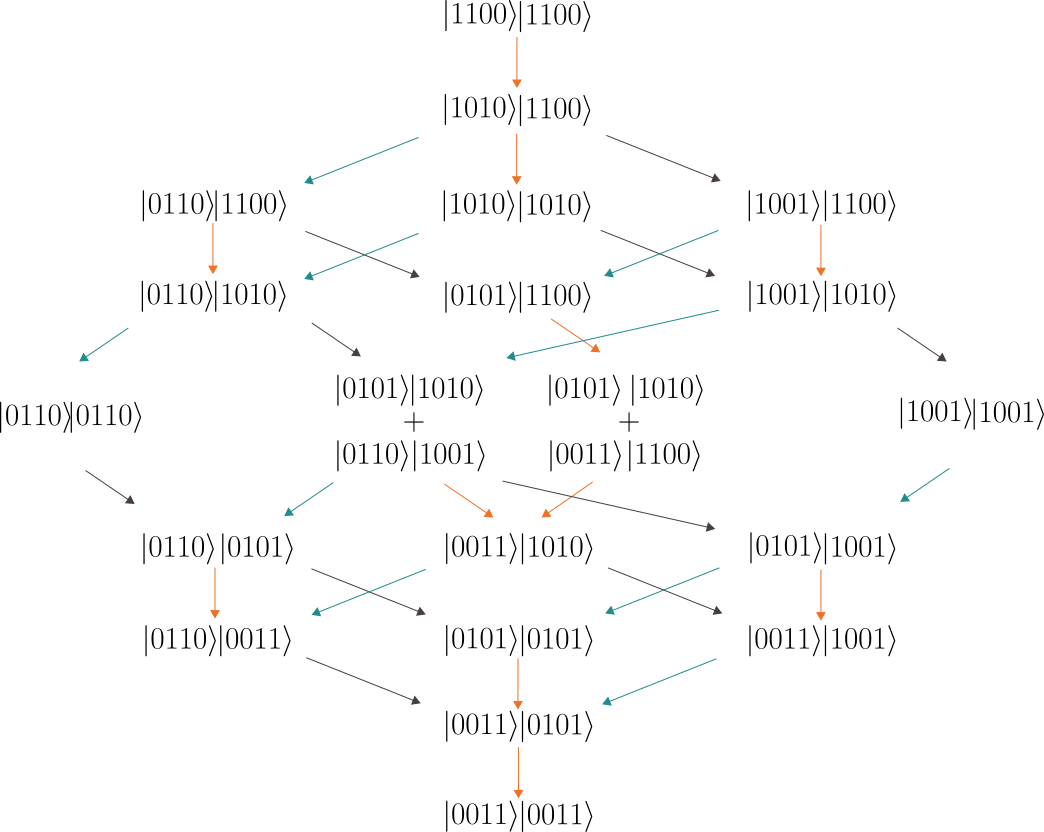
\includegraphics[scale=0.525]{img/hasse-diagram.png}
		\caption{The 20-dimensional irreducible symmetric subspace in ${\text 6_0 \otimes 6_0}$; The color of each arrow indicates the negative root \eqref{root-color} used to obtain the state. Every state is understood to be symmetrized.}
		\label{fig:hesse-diagram}
	\end{center}
\end{figure}
\begin{align}
\begin{split}
\ket{\beta} &= \frac{1}{\sqrt{6}} \Big( \ket{0101} \ket{1010}
	+ \ket{1010} \ket{0101}
	- \ket{0110} \ket{1001} \\
	&- \ket{1001} \ket{0110}
	- \ket{0011} \ket{1100}
	- \ket{1100} \ket{0011} \Big)
\end{split}
\end{align}
The singlets $\ket{1,0}$ and $\ket{35,0}$ are the linear combinations of $\ket{\alpha}$ and $\ket{\beta}$ annihilated by $a\dgg_1a\dgg_2 \otimes \id + \id \otimes a\dgg_1a\dgg_2$; they are
\begin{align}
\ket{\text 1,0} &= \frac{\ket{\alpha} + \sqrt{3} \ket{\beta} }{2}, &
\ket{\text 35,0} &= \frac{\sqrt{3} \ket{\alpha} - \ket{\beta} }{2}.
\end{align}
Note that $\ket{1,0}$, being simultaneously a $\gr{U}{4}$-singlet and the $\gr{Spin}{8}$-singlet, can also be obtained by the complex conjugation operator
\begin{align}
	\ket{1,0} &= -\id \otimes C_{8_+} \frac{1}{\sqrt{8}} \sum_j \ket{jj}.
\end{align}

Actually what we have found are singlets in $8_+ \otimes 8_+$, whereas the singlets in the Clebsch-Gordan coefficient $\Gamma_{\mu} = |\bra{\mu 0} (\ket{0000} \otimes \ket{0000})|$ are in $8_+ \otimes 8_+^*$. The two can be converted to one another by the complex conjugation operator:
\begin{align}
	\left| \prescript{}{8_+ \otimes 8_+^*}{}\!\!|\bra{\mu 0} (\ket{0000} \otimes \ket{0000}) \right|
		&= \left| \prescript{}{8_+ \otimes 8_+}{}\!\!\braket{\mu 0|\id \otimes C_{8_+}|0000} \otimes \ket{0000} \right| \\
		&= \left| \prescript{}{8_+ \otimes 8_+}{}\!\!|\bra{\mu 0} (\ket{0000} \otimes \ket{1111}) \right|.
\end{align}
Note that $\ket{0000}\ket{1111}$ is the highest weight state of $8_+ \otimes 8_+^*$ because $C_{8_+}$ swaps $a_j$ and $a\dgg_j$ ---that is, it swaps positive and negative roots of the Lie algebra. As a result,
\begin{align}\label{cg-coefficients}
	\Gamma_{\text 1}^2 &= \frac{1}{8}, & \Gamma_{\text 28}^2 &= \frac{1}{2}, & \Gamma_{\text 35}^2 &= \frac{3}{8}.
\end{align}


The spherical functions,
\begin{align}
	\rep_{\mu}(\Omega)_{00} &=
	\prescript{}{8_+\otimes 8_+}{}\!\!\braket{\mu 0|\rep_{8_+}\dgg(\Omega) \otimes U_{8_+}(\Omega)|\mu 0}_{8_+\otimes 8_+},
\end{align}
depend only the maximal abelian subgroup $A$ in the $KAK$ decomposition. Thus we can restrict $\rep_{8_+}$ to be
\begin{align}
\rep(\theta^+_{12},\theta^+_{34})_{8_+} &= \exp \left[ \frac{i}{2}(\theta^+_{12} Y^+_{12} + \theta^+_{34} Y^+_{34}) \right],
\end{align}
obtaining
\begin{align}
\rep_{1}(\theta^+_{12},\theta^+_{34})_{00} &= 1, \\
\rep_{28}(\theta^+_{12},\theta^+_{34})_{00} &= \frac{\cos(\theta^+_{12}) + \cos(\theta^+_{34})}{2}, \\
\rep_{35}(\theta^+_{12},\theta^+_{34})_{00} &= \frac{1+2\cos(\theta^+_{12}) \cos(\theta^+_{34})}{3}.
\end{align}
$(d_{\mu}/8)^{1/2} \rep_{\mu}(\Omega)_{00}$ are orthonormal functions with respect to the measure $d\Omega$ \eqref{measure}.

%------------------------------------
\subsection{Gaussian quasi-probability functions are negative}
%------------------------------------
The Q functions of Fermionic Gaussian states are
\begin{align}
\left| \braket{\Omega | \Omega'} \right|^2 &= \frac{1 + \cos\theta^+_{12} + \cos\theta^+_{34} + \cos\theta^+_{12}\cos\theta^+_{34}}{4},
\end{align}
which reduces to unity when $\Omega = \Omega'$. Alternatively, it is the product of spherical functions in the even spinor representation
\begin{align}
	U_8 (\theta_{12}^+) U_8 (\theta_{34}^+) &= \left( \frac{1 + \cos \theta_{12}^+}{2} \right) \left( \frac{1 + \cos \theta_{34}^+}{2} \right).
\end{align}
The quasi-probability function of the vacuum in the self-dual ($s=0$) representation is given by the formula
\begin{align}\label{brif-mann-wigner}
\mu_e (\Omega) &= \sum_{\mu} \Gamma_{\mu} \sqrt{ \frac{d_{\mu}}{d}} \rep_{\mu}(\Omega)_{00}.
\end{align}
The quasi-probability multiplied by the measure, depicted in Figure \ref{fig:wigner}, ends up taking negative values with an integrated negativity of $-0.47$. The measure vanishes on the line $\theta_{12}^+ = \theta_{34}^+$ and concentrates in the area where negativity occurs.
\begin{figure}[t]
	\begin{center}
	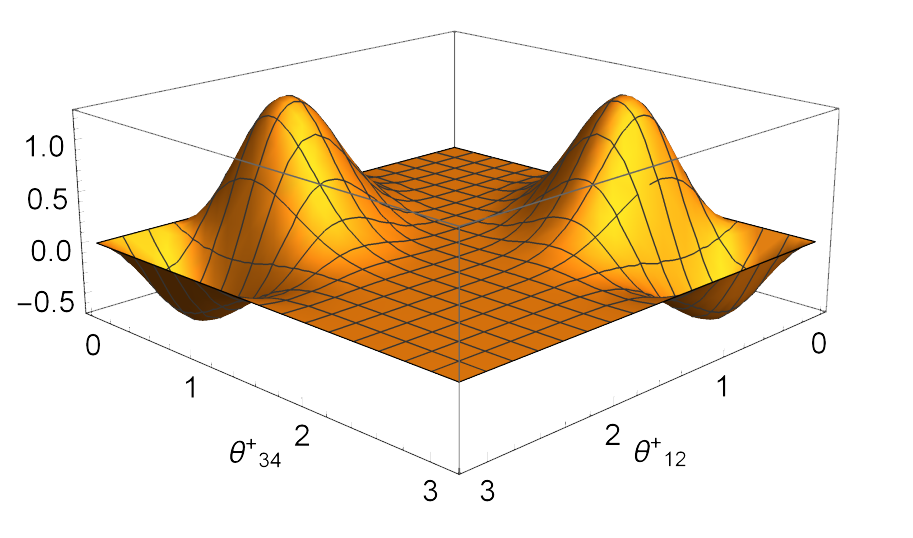
\includegraphics[scale=0.7]{img/SO-8-wigner.png}
	\caption{The Wigner function of pure fermionic Gaussian
		states, multiplied by the measure}
	\label{fig:wigner}
	\end{center}
\end{figure}

Let us briefly look at how the frame elements acquire negative eigenvalues. The frame is given by the formula
\begin{align}
F(\Omega,s) &= \sum_{\mu} \frac{1}{\Gamma_{\mu}^{1+s}} \left( \frac{d_{\mu}}{d} \right)^{(3+s)/2}
\int d\Omega'\,\rep_{\mu}(\Omega^{-1}\Omega')_{00} \ketbra{\Omega'}{\Omega'} \\
	&= \sum_{\mu} \left( \frac{d_{\mu}}{d\Gamma_{\mu}^2} \right)^{(1+s)/2} \frac{d_{\mu}}{d}
	\int d\Omega'\,\rep_{\mu}(\Omega^{-1}\Omega')_{00} \ketbra{\Omega'}{\Omega'}
\end{align}
By construction, any frame element can be obtained from another by the group action, so we can consider the frame element at $\Omega = 0$ for simplicity. In this case, it turns out that the integrals can be written in terms of $P_k$, the projection operators onto the $k$-particle sectors, as follows:
\begin{align}
	\int d\Omega\,\ketbra{\Omega}{\Omega} &= \id, \\
	\int d\Omega\,\rep_{28}(\Omega)_{00} \ketbra{\Omega}{\Omega} &= \frac{8}{28}\frac{P_0 - P_4}{2}, \\
	\int d\Omega\,\rep_{35}(\Omega)_{00} \ketbra{\Omega}{\Omega} &= \frac{8}{35} \left[ \frac{3}{8}(P_0 + P_4) - \frac{P_2}{8} \right].
\end{align}
Putting these together gives us
\begin{align}
F(0,s) &=	\frac{\id}{8}
	+ 7^{(1+s)/2} \frac{P_0 - P_4}{2}
	+ \left( \frac{35}{3} \right)^{(1+s)/2} \left[ \frac{3}{8}(P_0 + P_4) - \frac{P_2}{8} \right].
\end{align}
Setting $s = -1$, $P_2$ in the first and last term cancel exactly to reproduce the vacuum projection operator:
\begin{align}
F(0,-1) &= \left( \frac{1}{8} + \frac{1}{2} + \frac{3}{8} \right) P_0 + \left( \frac{1}{8} - \frac{1}{2} + \frac{3}{8} \right) P_4 = P_0.
\end{align}
As soon as $s>-1$, the negative contribution of $P_2$ in the last term wins and each frame element ceases to be a positive operator. For the self-dual frame $s=0$,
\begin{align}
F(0,0) &= \left( \frac{1}{8} + \frac{\sqrt{7}}{2} + \frac{\sqrt{105}}{8} \right) P_0 +  \left( \frac{1}{8} - \frac{\sqrt{7}}{2} + \frac{\sqrt{105}}{8} \right) P_4 +  \left( 1 - \sqrt{\frac{35}{3}} \right) \frac{P_2}{8} \\
&\approx 2.72 P_0 + 0.08 P_4 - 0.30 P_2,
\end{align}

%Thus,
%\begin{align}
%	F(\Omega,1) &= U(\Omega^{-1}) P_0 U(\Omega) \left( \frac{1}{8} + \frac{\sqrt{7}}{2} + \frac{\sqrt{105}}{8} \right) + P_4 \left( \frac{1}{8} - \frac{\sqrt{7}}{2} + \frac{\sqrt{105}}{8} \right) + \frac{P_2}{8} \left( 1 - \sqrt{\frac{35}{3}} \right)
%\end{align} 

%\chapter{Fermionic Phase Spaces}\label{ch:fermion-phase-space}
%\input{chapters/fermion-phase-space}

\chapter{Summary and Open Problems}\label{ch:open-problems}
\newcommand\rep{U}
\setlength\epigraphwidth{8.5cm}
\epigraph{I must finish what I've started, even if, inevitably, what I finish turns out not to be what I began.}{--- Salman Rushdie}
% Midnight's Children

This dissertation consists mainly of the following two research programs:
\begin{itemize}
	\item Find a generalization of the quantum Bochner's theorem, which simultaneously characterizes the set of valid quasi-probability distributions and the subset of non-negative ones in a given quasi-probability representation. (Chapter \ref{ch:commutative-phase-space})
	\item Find a quasi-probability representation that somehow reflects a classically simulatable subtheory of quantum theory. (Chapter \ref{ch:quasi-rep} and \ref{ch:matchgate})
\end{itemize}
Each program led us to what appears to be a different way to construct quasi-prob\-abi\-li\-ty representations out of groups. Let us summarize what we did.

After an overview of representation theory in Chapter \ref{ch:rep}, we formally introduce quasi-probability representations in Chapter \ref{ch:quasi-rep}. Focusing on finite-dimensional quantum systems, each quasi-probability representation is associated with a frame and a dual frame for $\mathbb{H}(\mathbb{C}^d)$, the real vector space of Hermitian operators over $\mathbb{C}^d$, where density operators and POVM elements live.

Valid probability densities can be characterized by properties of their Fourier transforms, the characteristic functions, by Bochner's theorem. The theorem easily generalizes by considering the notion of Fourier transform on a general group (\autoref{ch2:fourier-transform}). Given a unitary (ordinary or projective) representation $\{\rep(g)\}$ of a group $G$, we defined the quantum characteristic function of a density operator $\rho$ in Chapter \ref{ch:commutative-phase-space} to be the expectation value
\begin{align}
\phi_\rho(g) &=  \Tr[\rep(g) \rho].
\end{align}
For this quantity to be a Fourier transform of some quasi-probability distribution so that we could apply Bochner's theorem, the Fourier transform of the unitary operators $\{\rep(g)\}$ themselves must be a frame that defines a quasi-probability representation. We could not obtain such a (Hermitian) frame when $G$ is non-abelian. Instead, $\{\rep(g)\}$ must be a non-trivial projective representation of an abelian group $G$. Given such a representation, we showed that the resulting quasi-probability representation possesses a quantum Bochner's theorem (Theorem \ref{thm:main-bochner}). Further, we characterized the form that such a group $G$ must take and gave examples of quasi-probability representations with a quantum Bochner's theorem in low dimensions, which includes Gibbons' \cite{gibbons_discrete_2004} and Gross' phase space representations \cite{gross_hudsons_2006}.

The construction by Brif and Mann \cite{brif_phase-space_1999} outlined in \autoref{ch3:SW} is an answer to how to build quasi-probability representations from non-abelian groups. One of our contributions is a more deductive derivation of Brif and Mann's construction starting from the kernel
\begin{align}
	\rker{ss'}(\Omega,\Omega') \coloneqq \Tr [F(\Omega,s) F(\Omega',-s')]
\end{align}
that relates $G$-covariant frames at different values of the parameter $s$:
\begin{align}
	F(\Omega,s) &= \int d\Omega'\,\rker{ss'}(\Omega,\Omega') F(\Omega',s').
\end{align}
In particular, $F(\Omega,-1)$ is stipulated to be the $G$-coherent state $\ketbra{\Omega}{\Omega}$. Then the Stratonovich-Weyl (SW) correspondence and the differentiability of $F(s)$ with respect to $s$ imply the essential uniqueness of the frames, as stated in Theorem \ref{thm:brif-mann-frame}. In particular, the frame for $s=0$ is unique. We call these frames SW frames and the representations SW representations. 

The construction process commences by choosing three ingredients: a Lie group $G$, its unitary representation $\rep$ on a Hilbert space $\hilb$, and a fiducial state $\ket{e} \in \hilb$. If $\ket{e}$ is the highest weight state of $\rep$, then the phase space has more structure, namely the symplectic and K{\"a}hler structures (Appendix \ref{app:kahler}). The $G$-coherent states
\begin{align}
	\ket{\Omega} = \rep(\Omega)\ket{e}
\end{align}
are identified with phase points $\Omega = gK$ in the phase space $G/K$, where $K$ is the stabilizer of $\ketbra{e}{e}$. We showed that the quasi-probability functions of $G$-coherent states (for any $s$) are drawn, not from the entire space $L^2(G/K)$ of square-integrable functions on $G/K$, but only from irreps $\{V_{\mu}\}$ that make up the space of linear operators over $\hilb$
\begin{align}
\text{End}(\hilb) &\stackrel{G}{\simeq} \bigoplus_{\mu \in \hat{G}} \bigoplus^{n_{\mu}} V_{\mu}.
\end{align}
In other words, only low frequency components enter the quasi-probability functions of $G$-coherent states.

The construction was then applied to the classically simulatable problem of fermionic linear optics or equivalently, by the Jordan-Wigner transformation, nearest neighbor (N.N.) matchgates in Chapter \ref{ch:matchgate}. The $\gr{SO}{2n}$-coherent states are the $n$-mode (pure) fer\-mi\-on\-ic Gaussian states generated from the highest weight state of the even spinor representation $2^{n-1}_+$, the vacuum. In this case, the stabilizer of the vacuum is the number-preserving subgroup isomorphic to $\gr{U}{n}$, which can be characterized explicitly as a subgroup consisting of all matrices that are both orthogonal and symplectic. $\homsp{SO}{2n}{U}{n}$ is not just any homogeneous space; it is symmetric and hence multiplicity-free (\autoref{ch2:gelfand}). Thus, there is a unique (zonal) spherical function associated to each inequivalent irrep $V_{\mu}$ and, as shown in \autoref{ch3:construction}, the quasi-probability functions of the $G$-coherent states are spanned by these spherical functions. Finally, we arrived at the fact that the Gaussian quasi-probabilities are negative. Therefore, anyone who would like to come up with a fermionic quasi-probability representation that exhibits non-negative quasi-probabilities for the Gaussian states and the Gaussian measurements would need to break some assumptions of the SW representations.

We would have a cleaner connection to classical simulatability if we had found a non-negative subtheory for matchgate computation. One possibility is that no such subtheory exists. This is the case for multi-qubit stabilizer circuits, where the three-qubit GHZ states and Pauli measurements demonstrate (Kochen-Specker) contextuality; thus, it is contextual in the generalized sense of Spekkens \cite{spekkens_negativity_2008} and therefore has no non-negative subtheory. (Though, there is no natural notion of locality in our $n$-qubit phase space, not being the Cartesian product of a phase space for each individual qubit.) During the course of this project, we were informed by Brod \cite{brod-CHSH} that four-qubit N.N. matchgates can be used to violate the Bell-CHSH inequality. Thus, it is likely that matchgate computation also has no non-negative subtheory. %Proving contextuality using the Mermin-Peres square also seems like a dead end because matchgate does not allow even a very simple correlated measurements such as the $Z$-parity measurement $ZZ$, as it indeed promotes N.N. matchgates to universality.
Nevertheless, outcome probabilities from negative quasi-probabilities can still be efficiently estimated as long as the negativity does not grow too fast \cite{pashayan_estimating_2015}. Thus, we would like to have a uniform construction of our fermionic quasi-probability representations for all numbers of modes $n$. We have made some progress on this front that will be reported elsewhere; for example, we could calculate the singlets and spherical functions for any $n$, and we believe that the frame operator at the origin $\Omega=0$ can be obtained from just the $\gr{U}{n}$-singlets and the complex conjugation operators. But at the time of writing, we do not yet know how to directly obtain the integrated negativity of Gaussian quasi-probability distributions, as it seems to require actually doing the integral for each $n$ and every $n$. %Simulating quasi-probabilities on a computer also mean that we want to discretize the phase space. There is a numerically stable way to discretize a sphere into symmetric grids. Is there something like that for higher dimensional homogeneous spaces?

A broader perspective one can take going forward in this project is the study of general SW phase spaces in their own rights. SW phase spaces covariant to ``classical", restricted dynamics (subgroups of the full unitary group) may provide novel theoretical tools to think about physics akin to the Wigner function. There are other physically significant phase spaces for fermions identified in \cite{zhang_coherent_1990} such as the number-preserving phase space,
\begin{align}
\faktor{\gr{U}{n}}{\gr{U}{k} \times \gr{U}{n-k}},\nonumber
\end{align} 
and the parity-non-preserving phase space $\homsp{SO}{2n+1}{U}{n}$. For bosons, the construction of SW phase spaces when applied to the Weyl-Heisenberg group yields the Wigner, P, and Q functions as well as all the quantum optical $s$-parametrized quasi-probability representations \cite{brif_phase-space_1999}. Let us call these representations the \emph{linear} bosonic representations. Among them, the Wigner function, and only the Wigner function, is covariant with respect to the symplectic group $\gr{Sp}{2n,\mathbb{R}}$. But one could also have \emph{quadratic} phase spaces covariant with respect to the full symplectic group $\gr{Sp}{2n,\mathbb{R}}$ for every $s$. How do the quadratic and linear SW representations relate to one another? (The Wigner function is singled out from other linear bosonic representations by the \emph{marginal property} \cite{bertrand_tomographic_1987}: integrating the Wigner function $\mu_{\rho}$ along the line $aq+bp=c$ yields the probability to obtain the result $c$ upon measuring the observable $aQ+bP$. It is far from clear whether the Wigner function can be retrieved from the construction of quadratic bosonic representations.) For every SW phase space, one can ask for the characterization of positive (and valid) quasi-probability distributions:
\begin{itemize}
	\item Do the $G$-coherent states possess positive quasi-probability distributions?
	\item Is there any pure state that has a positive quasi-probability distribution?
	\item When do mixed states, for instance, thermal states at certain temperatures, have positive quasi-probability distributions?
	\item Is there some version of a quantum Bochner's theorem that characterizes SW quasi-probability distributions by their Fourier transforms? (How exactly is the abelian construction in Chapter \ref{ch:commutative-phase-space} a special case of the Brif and Mann's construction? Is there a similar construction that applies to finite groups as well?)
\end{itemize}
Another open question is the relation between our fermionic phase spaces and other existing fermionic phase spaces, for instance, those that employ Grassmann variables \cite{cahill_density_1999,dalton2014phase} or the Q functions in \cite{corney_gaussian_2006-1,corney_gaussian_2006,rosales-zarate_probabilistic_2015} (which actually have support over a much larger, complexified phase space covariant under $\gr{SO}{4n}$, not $\gr{SO}{2n}$).

Still lacking is an operational significance of SW phase spaces---something that makes the Wigner function an appealing way to think about homodyne and heterodyne measurements and quantum tomography. The two-dimensional slice of the full twelve-dimensional Wigner function in Figure \ref{fig:wigner} does not give a probability density upon integrating out a variable in any obvious way. Could the symplectic structure on the phase spaces play any role in ferreting out the marginal structure? Elaborating further structures, expected or unexpected, of SW phase spaces is necessarily the key to more applications of them.



%{\cmc You should now read through this conclusion and see if you like it and whether it can be made more user-friendly by adding on some more words.  In particular, you really can't end it with a question.  You need to end with some other kind of summary, a sort of summary of the questions.  Is there a theme to these questions, or are they just randomly pulled out of a hat?} 

\backmatter
\begin{appendices}

\chapter{Proof of the Discrete Hudson's Theorem}\label{app:hudson}
We provide here a complete proof of the discrete Hudson's theorem, following a sketch in an unpublished talk by Gross \cite{gross2015coogee}.\footnote{I am grateful to Marcus Appleby for sharing his extensive knowledge on discrete Wigner functions and pointing out the group property of the frame for Gross's Wigner function.}

Hudson's theorem states that the Wigner function of a pure state is positive if and only if it is Gaussian \cite{hudson_when_1974}. The theorem in the multi-mode scenario and other generalizations was given in \cite{soto_when_1983,toft_hudsons_2006} and references therein. In the discrete case we have

\begin{theorem}{\normalfont (Discrete Hudson's theorem)}
	Gross' Wigner function \eqref{ch4:gross-wigner-function} of a pure state $\ket{\psi}$ is positive if and only if $\ket{\psi}$ is a stabilizer state
	{\normalfont \cite{gross_hudsons_2006,gross_non-negative_2007}.}
\end{theorem}

\emph{Stabilizer states} were originally defined for multiple qubits \cite{gottesman_stabilizer_1997} and have a plethora of applications in quantum error correction and quantum computation \cite{fujii2015quantum}.
In odd dimensions, they have the following equivalent characterizations:
\begin{enumerate}
	
	\item\label{def-stabilizer} Each stabilizer state is a joint eigenvector of a \emph{stabilizer subgroup} -- a maximal abelian subgroup of the generalized Pauli group $\mathcal{P}_d$.
	
	\item\label{clifford-orbit} Stabilizer states are the orbit of the state $\ket{0}$ under the Clifford group.
	
	\item\label{gaussian-wave-function} Their wave functions have a Gaussian form in the standard basis $\{\ket{m}\mid m=0,\dots, d-1 \}$
	\begin{align}
	\psi(m) = \omega^{mAm + bm},
	\end{align}
	where $A$ is a symmetric matrix with entries in $\mathbb{Z}_d$ and $b \in \mathbb{Z}_d$. %{\cmc Is there a difference between the sub and superscript $d$?}
	
\end{enumerate}
Properties \ref{clifford-orbit} and \ref{gaussian-wave-function} especially affirm the status of stabilizer states as the natural discrete analogue of Gaussian states.

To prove the discrete Hudson's theorem in one direction, one computes the discrete Wigner function of all stabilizer states directly and observes that they are positive. In fact, the support of a stabilizer state always lies on a line (as defined in finite geometry) \cite{gross_hudsons_2006}, so they are more like infinitely squeezed states.

A short proof in the other direction given in an unpublished talk by Gross \cite{gross2015coogee} can be summarized as follows: a positive discrete Wigner function of
a pure state simultaneously maximizes the 2-norm and minimizes the 1-norm, forcing it to be a stabilizer state.
\begin{lemma}
	\label{lem:supp_size}A positive Wigner function $\mu_{\psi}$ of
	a pure state $\rho= \ketbra{\psi}{\psi}$ must be constant on
	its support of size $d$.
\end{lemma}
\begin{proof}
	We want to bound the 2-norm of $\rho$,
	\begin{align}
	\norm \rho_{2}^{2} & = \Tr (\rho^{\dagger}\rho)
	= \sum_{j,k} |\rho_{jk}|^{2}.
	\end{align}
	Every displacement operator except $\id$ has zero trace, so the trace of $A(0,0)$ and thus every phase point operator is 1. Moreover, $ \{ A({\bf u})/\sqrt{d} \} $ is an orthonormal basis because $A({\bf u})$ squares to the identity. Therefore,
	\begin{align}
	\frac{1}{d} \le  \sum_{j,k} |\rho_{jk}|^{2} &= \frac{1}{d} \sum_{{\bf u}} \left| \Tr [A({\bf u}) \rho] \right|^2 \le 1.
	\end{align}
	$\rho$ is a pure state if and only if $ \norm \rho _{2}^{2} = \Tr (\rho^2) = 1$, which means that on the one hand,
	\begin{align}
	\sum_{{\bf u}} |\braket{\psi|A({\bf u})|\psi}|^2 &= d, \label{eq:2-norm}
	\end{align}
	i.e. the 2-norm is maximized. On the other hand,
	\begin{align}
	\sum_{{\bf u}} \braket{\psi|A({\bf u})|\psi} &= d.
	\end{align}
	Every term in the sum is positive if and only if its 1-norm is minimized
	\begin{align}
	\sum_{{\bf u}} |\braket{\psi|A({\bf u})|\psi}| &= d.\label{eq:1-norm}
	\end{align}
	Each term in the sum can be bounded by the sum of the product of the singular values using von Neumann's trace inequality:
	\begin{align}
	|\Tr(AB)| &\le \sum_j a_j b_j,\label{eq:trace_ineq}
	\end{align}
	where $a_{j}$ and $b_{j}$ are singular values of $A$ and $B$ respectively,
	ordered by their magnitudes. The bound is saturated if and only if $A$ and
	$B$ are normal and commute. Since $\rho$ is a rank-one projection
	operator, we only need the largest singular value of $A({\bf u})$,
	which is 1,
	\begin{align}
	|\braket{\psi|A({\bf u})|\psi}| &\le \norm{A({\bf u})}_{\infty} = 1\label{eq:baby_holder_ineq}
	\end{align}
	But if this bound is not saturated, the 2-norm will not reach the
	maximum. To saturate the bound, $\mu_{\rho}$ can have a support only
	on $d$ points and $\ket{\psi}$ must be a joint eigenvector of $d$
	phase point operators.
\end{proof}	

\noindent In particular, $\ket{\psi}$ is an eigenvector of every product of these $d$ phase point operators, which makes it also an eigenvector of some displacement operators because
\begin{align}\label{phase-point-clifford}
	A({\bf u}) A({\bf v})
		&= \left( D\dgg ({\bf u}) A({\bf 0}) D ({\bf u}) \right)
			\left( D\dgg ({\bf v}) A({\bf 0}) D ({\bf v}) \right) \nonumber \\
		&= \omega^{-[{\bf u,v}]/2} D({\bf -u})	\left[ A({\bf 0}) D ({\bf u-v}) A({\bf 0}) \right] D ({\bf v}) \nonumber \\
		&= \omega^{-[{\bf u,v}]/2} D({\bf -u})D ({\bf v-u}) D ({\bf v}) \nonumber \\
		&= \omega^{-2 [{\bf u,v}]} D(2{\bf v} - 2{\bf u}).
\end{align}
When ${\bf w = v-u} \neq 0$, $2{\bf w}$ is never zero since $d$ is odd. So for a given ${\bf w}$, $\ket{\psi}$ is an eigenvector of $d$ commuting displacement operators $\{ \id, D({\bf w}), \dots, D^{d-1}({\bf w}) \}$ and there can be no more than $d$ commuting displacement operators since $D({\bf w})$ has period $d$. $\ket{\psi}$ is therefore a stabilizer state and the discrete Hudson's theorem is proved. 

\chapter{Measure on Homogeneous K{\"a}hler Manifolds}\label{app:kahler}
The integration measure on the phase space can be obtained from the line element denoted by $ds^2$. The $d$-dimensional Euclidean line element is, for example,
\begin{align}
	ds^2 &= \sum_{j=1}^d dx^j \otimes dx^j.
\end{align}
The superscript signifies that $dx^j$ are dual vectors (i.e. forms).
For a vector $\ket{\psi} = \sum_j^dz_j \ket{e_j}$ in a complex vector space $\mathbb{C}^d$, a small displacement
\begin{align}
	\ket{d\psi} &= \sum_{j=1}^d dz^j \ket{e_j}
\end{align}
gives rise to the line element
\begin{align}
	ds^2 &= \braket{d\psi|d\psi} = \sum_{j=1}^d dz^j \otimes dz^{j*}.
\end{align}
The inner product $\braket{d\psi|d\psi}$ in $\mathbb{C}^d$ does not give a line element on the complex projective space $\mathbb{C}P^{d-1}$; one has to project it back to $\mathbb{C}P^{d-1}$ by subtracting off the part orthogonal to the manifold:
\begin{align}
ds^2 &= (\bra{d\psi} - \braket{d\psi | \psi} \bra{\psi} )( \ket{d\psi} - \ket{\psi} \braket{\psi | d\psi} ) \\
&= \braket{d\psi | d\psi} -  \left| \braket{\psi | d\psi} \right|^2,
\end{align}
obtaining the celebrated \emph{Fubini-Study metric} \cite{caves2001measures}.

For a $d$-level system, a manifold of $G$-coherent states is a submanifold of $\mathbb{C}P^{d-1}$.
Suppose that we have a sequence $U=U_n \cdots U_1$ of unitary operators $U_j = \exp(i\theta^{\mu} J_j)$ that generates a $G$-coherent state $\ket{\Omega}$ from the fiducial state $\ket{e}$:
\begin{align}
	\ket{\Omega} &= U\ket{e} = U_n \cdots U_1 \ket{e},
\end{align}
then a small displacement is given by
\begin{align}
\ket{d\Omega} &= dU(\Omega) \ket{e} = dU(\Omega) U^{-1}(\Omega) \ket{\Omega}
= iX_j \ket{\Omega} d\theta^j,
\end{align}
where
\begin{align}
i X_j &= U_n \cdots U_{j+1} J_j U_{j+1}\dgg \cdots U_n\dgg,
\end{align}
and repeated indices are summed over.
The line element for the submanifold of $G$-coherent state induced by the Fubini-Study metric is
\begin{align}
ds^2 &= \left( \braket{\Omega |X_{j} X_{k}| \Omega} - \braket{\Omega | X_{j} | \Omega} \braket{\Omega | X_{k} | \Omega} \right) d\theta^{j} \otimes d\theta^{k}, \\
	&=  \left( \braket{e|Y_{j}(\Omega) Y_{k}(\Omega)|e} - \braket{e| Y_{j}(\Omega) |e} \braket{e| Y_{k}(\Omega) |e} \right) d\theta^{j} \otimes d\theta^{k},
\end{align}
where $Y_{j}(\Omega)$ is the displaced generator
\begin{align}
i Y_{j} = U_1\dgg \cdots U_{j-1}\dgg J_{j} U_{j-1} \cdots U_1.
\end{align}
The (symmetric) real part of $ds^2$ is a Riemannian metric
\begin{align}
	g_{jk} &= \frac{1}{2} \braket{\Omega | \{X_j, X_k\} | \Omega} - \braket{\Omega | X_j | \Omega} \braket{\Omega | X_k | \Omega},
\end{align}
and the measure is
\begin{align}
	d\Omega &= \sqrt{|\det g_{jk}|} d\theta^j \otimes d\theta^k.
\end{align}

%The manifold of Gaussian states is not only even-dimensional but also K{\"a}hler, being an orbit of the highest weight state \cite{onofri_note_1975}. The fact that the complex projective space $\mathbb{C}^{2^n-1}$ is also K{\"a}hler with the Fubini-Study metric as the Hermitian metric suggests that we look at the induced metric on the phase space:

In $\mathbb{C}P^{d-1}$ and any of its ``complex" submanifolds, something special occurs. Recall that in $\mathbb{C}^d \simeq \mathbb{R}^{2d}$ (which is also the classical phase space), we have the Hermitian inner product
\begin{align}
	\braket{u,v} &= \sum_{j=1}^d u_j^* v_j,
\end{align}
the symmetric inner product
\begin{align}
	g(x,y) &= \sum_{j=1}^{2d} x_j y_j,
\end{align}
and the symplectic bilinear form
\begin{align}
	\omega(x,y) &= g(Jx, y) = \sum_{j=1}^{2d} \left( x_j y_{d+j} - x_{d+j} y_j \right),
\end{align}
where
\begin{align}\label{ch3:eq:almost-complex-structure}
	J &= \begin{pmatrix}
	{\huge 0} & -\id \\
	\id & {\huge 0}
	\end{pmatrix}
\end{align}
plays the role of the imaginary unit $i$. The three bilinear forms fit together in the identity
\begin{align}
	\braket{u,v} &= g(u,v) + i\omega(u,v),
\end{align}
where $u$ and $v$ on the right hand side are understood to be $2d$-long vectors of real and imaginary parts of $u$ and $v$. We would like to generalize this scenario to a more general manifold that cannot be covered by a single chart. Let $J$ be a $(1,1)$-tensor field on a real, even-dimensional manifold $M$ that squares to minus the identity
\begin{align}
	J^2 &= -\id.
\end{align}
At each point $p$ in $M$, $J_p$ has a diagonal form
\begin{align}
	J_p &= \begin{pmatrix}
		i\id & {\huge 0} \\
		{\huge 0} & -i\id
		\end{pmatrix}
\end{align}
in the basis
\begin{align}
	Z_j = X_j + iX_{d+j}, &&
	Z^*_j = X_j - iX_{d+j},
\end{align}
of the complexified tangent space.
If we can keep the diagonal form of $J_p$ while varying the base point $p$ by a coordinate transformation of $\{Z_j\}$ that depends only on $\{Z_j\}$ and not $\{Z^*_j\}$ (that is, the transition function is holomorphic), then the manifold $M$ is called \emph{complex}. A complex manifold always admit a Hermitian metric $\braket{\, ,\,}$ such that
\begin{align}
	\braket{u,v} &= g(u,v) + i\omega(u,v),
\end{align}
with $g$ a Riemannian metric and $\omega$ a non-degenerate, anti-symmetric bilinear form. When the form is closed,
\begin{align}
	d\omega &= 0,
\end{align}
---that is, when $\omega$ is a symplectic form---the manifold is \emph{K{\"a}hler} \cite{BZ,kobayashi1969foundations,nakahara2003geometry}.
Complex projective spaces are exemplars of K{\"a}hler manifolds, with the Fubini-Study metric as the Hermitian metric. Every complex submanifold of a complex projective space inherits the K{\"a}hler structure with the induced metric \cite[Example 6.7, p.164]{kobayashi1969foundations}. More generally, any orbit of a highest weight state, thus any Gilmore's phase space, is guaranteed to be K{\"a}hler \cite{onofri_note_1975}.
On a K{\"a}hler manifold, the $n$th anti-symmetric power of the symplectic form
\begin{align}
	d\Omega &= \frac{1}{n!}\bwedge^n \omega,
\end{align}
agrees with the integration measure obtained from the metric. 

To summarize, when the phase space is K{\"a}hler, the Riemannian metric and the symplectic form are
\begin{align}
	g_{jk} &= \frac{1}{2} \braket{\Omega | \{X_j, X_k\} | \Omega} - \braket{\Omega | X_j | \Omega} \braket{\Omega | X_k | \Omega}, \\
	\omega_{jk} &= \frac{1}{2i} \braket{\Omega | [X_j, X_k] | \Omega},
\end{align}
and both lead to the same integration measure $d\Omega$. 

\end{appendices}

\bibliographystyle{abbrv-alpha-letters-links}
\bibliography{bibliography/main-bib,bibliography/zotero-intro,bibliography/rep-theory,bibliography/zotero-fermion,bibliography/zotero-quasi-rep,bibliography/zotero-tensor-network}
\bibliographystyle{plain}

\end{document}
